\chapter{范畴论基础}

\minitoc

本章提供书中使用的一些范畴论概念和结论, 而不是成体系的范畴论教程.

\section{$2$-范畴}

\label{section-2-categories}

假设读者已经熟悉范畴, 函子, 自然变换的概念.

\begin{definition}
	[label={2-categories}]
	{(严格 $2$-范畴)}
	\emph{严格 $2$-范畴}是指 $\mathsf {Cat}$-充实范畴, 其中 $\mathsf {Cat}$ 是 (小) 范畴的范畴. 具体地说, 一个严格 $2$-范畴 $\mathcal C$ 包含如下资料,
	\begin{itemize}
		\item 一族\emph{对象} $A,B,C,\cdots$;
		\item 对每两个对象 $A,B$ 有一个\emph{范畴} $\operatorname{Hom}_{\mathcal C}(A,B)$, 其中的对象称为 $\mathcal C$ 的\emph{态射}, 态射称为 $\mathcal C$ 的 \emph{$2$-态射};
		\item 对每三个对象 $A,B,C$ 有一个函子 ``复合'' $\circ\colon \operatorname{Hom}_{\mathcal C}(B,C)\times \operatorname{Hom}_{\mathcal C}(A,B) \to \operatorname{Hom}_{\mathcal C}(A,C)$;
		\item 对每个对象 $A$ 有一个对象 ``恒等'' $i_A\colon 1\to \operatorname{Hom}_{\mathcal C}(A,A)$;
	\end{itemize}
	满足如下严格的结合律,\footnotemark{}
	% https://q.uiver.app/#q=WzAsNCxbMSwwLCJcXG9wZXJhdG9ybmFtZXtIb219KEIsRClcXHRpbWVzXFxvcGVyYXRvcm5hbWV7SG9tfShBLEIpIl0sWzAsMCwiXFxvcGVyYXRvcm5hbWV7SG9tfShDLEQpXFx0aW1lc1xcb3BlcmF0b3JuYW1le0hvbX0oQixDKVxcdGltZXNcXG9wZXJhdG9ybmFtZXtIb219KEEsQikiXSxbMCwxLCJcXG9wZXJhdG9ybmFtZXtIb219KEMsRClcXHRpbWVzXFxvcGVyYXRvcm5hbWV7SG9tfShBLEMpIl0sWzEsMSwiXFxvcGVyYXRvcm5hbWV7SG9tfShBLEQpIl0sWzEsMiwiXFxjaXJjX3tBLEIsQ30iLDJdLFsyLDMsIlxcY2lyY197QSxDLER9IiwyXSxbMSwwLCJcXGNpcmNfe0IsQyxEfSJdLFswLDMsIlxcY2lyY197QSxCLER9Il1d
	\[\begin{tikzcd}[ampersand replacement=\&]
		{\operatorname{Hom}(C,D)\times\operatorname{Hom}(B,C)\times\operatorname{Hom}(A,B)} \& {\operatorname{Hom}(B,D)\times\operatorname{Hom}(A,B)} \\
		{\operatorname{Hom}(C,D)\times\operatorname{Hom}(A,C)} \& {\operatorname{Hom}(A,D)}
		\arrow["{\circ_{A,B,C}}"', from=1-1, to=2-1]
		\arrow["{\circ_{A,C,D}}"', from=2-1, to=2-2]
		\arrow["{\circ_{B,C,D}}", from=1-1, to=1-2]
		\arrow["{\circ_{A,B,D}}", from=1-2, to=2-2]
	\end{tikzcd}\]
	以及如下严格的单位律.
	\[\begin{tikzcd}[ampersand replacement=\&]
		{\operatorname{Hom}(A,B)} \&\& {\operatorname{Hom}(A,B)} \\
		{\operatorname{Hom}(B,B)\times\operatorname{Hom}(A,B)} \& {\operatorname{Hom}(A,B)} \& {\operatorname{Hom}(A,B)\times\operatorname{Hom}(A,A)}
		\arrow["{\operatorname{id}}", from=1-1, to=2-2]
		\arrow["{i_B\times \operatorname{id}}"', from=1-1, to=2-1]
		\arrow["{\circ_{A,B,B}}"', from=2-1, to=2-2]
		\arrow["{\circ_{A,A,B}}", from=2-3, to=2-2]
		\arrow["{\operatorname{id}}"', from=1-3, to=2-2]
		\arrow["{\operatorname{id}\times i_A}", from=1-3, to=2-3]
	\end{tikzcd}\]
\end{definition}
\footnotetext{``严格'' 的含义是, 这张图中两条路径给出的函子严格相等 (也即构成 $1$-范畴 $\mathsf {Cat}$ 中的交换图). 图中我使用了 ``三个范畴的乘积'', 而更严格的写法应该分别写出两种顺序的乘积 $(-\times -)\times -$ 与 $-\times (-\times -)$, 并以幺半范畴 $\mathsf {Cat}$ 中的结合子相连接 (例如定义 \ref{2-functor} 中就完整地写出了结合子). 类似地, 后面的图中我使用了 $\operatorname{Hom}(A,B)\times 1$ 与 $\operatorname{Hom}(A,B)$ 的同构, 而这也应该理解为幺半范畴中的单位子.}

严格 $2$-范畴的概念不够好, 因为我们不应该要求两个函子\emph{相等}, 而是应该要求指定一个\emph{自然同构}.\footnote{在范畴的 $2$-范畴 $\mathcal Cat$ 中, $1$-态射 (函子) 之间不能谈论相等, 只能谈论自然同构; 而 $2$-态射 (自然变换) 之间可以谈论相等. 一般地, 对于 $n$-范畴 (无论何种模型) 中小于 $n$ 阶的态射, 我们都不能谈论相等, 只能谈论等价; 而对于 $n$-范畴中的 $n$-态射则有相等的概念, 如集合中的元素, 范畴中的态射, $2$-范畴中的 $2$-态射等等.}

\begin{definition}
	[label={weak-two-category}]
	{(弱 $2$-范畴)}
	一个弱 $2$-范畴 (以下简称 \emph{$2$-范畴}, 又叫 \emph{bicategory}) $\mathcal C$ 包含如下资料,
	\begin{itemize}
		\item 一族\emph{对象} $A,B,C,\cdots$;
		\item 对每两个对象 $A,B$ 有一个\emph{范畴} $\operatorname{Hom}_{\mathcal C}(A,B)$, 其中的对象称为 $\mathcal C$ 的\emph{态射}, 态射称为 $\mathcal C$ 的 \emph{$2$-态射};
		\item 对每三个对象 $A,B,C$ 有一个函子 ``复合'' $\circ\colon \operatorname{Hom}_{\mathcal C}(B,C)\times \operatorname{Hom}_{\mathcal C}(A,B) \to \operatorname{Hom}_{\mathcal C}(A,C)$;
		\item 对每个对象 $A$ 有一个对象 ``恒等'' $i_A\colon 1\to \operatorname{Hom}_{\mathcal C}(A,A)$;
		\item 对每两个对象 $A,B$ 有两个\emph{自然同构} ``\emph{单位子} (unitor)''
		$$\rho_{A,B}\colon (-\circ i_A)  \overset{\simeq}{\to}  (-),\ 
		\lambda_{A,B} \colon (i_B\circ -) \overset{\simeq}{\to}  (-);$$
		\item 对每四个对象 $A,B,C,D$ 有一个\emph{自然同构} ``\emph{结合子} (associator)''
		$$\alpha_{A,B,C,D}\colon \big((-\circ -) \circ {-}\big) \overset{\simeq}{\to} \big({-}\circ (- \circ -)\big);$$%\colon \operatorname{Hom}(C,D)\times\operatorname{Hom}(B,C)\times\operatorname{Hom}(A,B)\to \operatorname{Hom}(A,D);$
	\end{itemize}
	满足\emph{五边形恒等式}, 又叫结合律的\emph{融贯性} (coherence).
	% https://q.uiver.app/#q=WzAsNSxbMCwxLCIoKGZnKWgpayJdLFsyLDIsIihmKGdoKSlrIl0sWzQsMiwiZigoZ2gpaykiXSxbNiwxLCJmKGcoaGspKSJdLFszLDAsIihmZykoaGspIl0sWzAsNF0sWzAsMV0sWzEsMl0sWzQsM10sWzIsM11d
	\[\begin{tikzcd}[ampersand replacement=\&,column sep=-1.7em,row sep=2em]
		\&\&\& {(-\circ -)\circ(-\circ -)} \\
		{((-\circ -)\circ -)\circ -} \&\&\&\&\&\& {-\circ(-\circ(-\circ -))} \\
		\&\& {(-\circ (-\circ -))\circ -} \&\& {-\circ((-\circ -)\circ -)}
		\arrow["\alpha", from=2-1, to=1-4]
		\arrow["\alpha"', from=2-1, to=3-3]
		\arrow["\alpha"', from=3-3, to=3-5]
		\arrow["\alpha", from=1-4, to=2-7]
		\arrow["\alpha"', from=3-5, to=2-7]
	\end{tikzcd}\]
	以及\emph{三角形恒等式}, 又叫单位律的融贯性.
	% https://q.uiver.app/#q=WzAsMyxbMCwwLCIoZmkpZyJdLFsxLDAsImYoaWcpIl0sWzEsMSwiZmciXSxbMCwxLCJcXGFscGhhIl0sWzAsMiwiXFxyaG8iLDJdLFsxLDIsIlxcbGFtYmRhIl1d
	\[\begin{tikzcd}[ampersand replacement=\&]
		{(-\circ i)\circ -} \& {-\circ (i\circ -)} \\
		\& -\circ -
		\arrow["\alpha", from=1-1, to=1-2]
		\arrow["\rho"', from=1-1, to=2-2]
		\arrow["\lambda", from=1-2, to=2-2]
	\end{tikzcd}\]
\end{definition}

\begin{remark}
	{(横向复合, ``须'')}
	复合 $\circ\colon \operatorname{Hom}_{\mathcal C}(B,C)\times \operatorname{Hom}_{\mathcal C}(A,B) \to \operatorname{Hom}_{\mathcal C}(A,C)$ 的函子性给出了 $2$-态射的\emph{横向复合}
	\[\begin{tikzcd}[ampersand replacement=\&,]
		A \& B \& C
		\arrow[""{name=0, anchor=center, inner sep=0}, "f", bend left, from=1-1, to=1-2]
		\arrow[""{name=1, anchor=center, inner sep=0}, "{f'}"', bend right, from=1-1, to=1-2]
		\arrow[""{name=2, anchor=center, inner sep=0}, "g", bend left, from=1-2, to=1-3]
		\arrow[""{name=3, anchor=center, inner sep=0}, "g'"', bend right, from=1-2, to=1-3]
		\arrow["\alpha", shorten <=2pt, shorten >=2pt, Rightarrow, from=0, to=1]
		\arrow["\beta", shorten <=2pt, shorten >=2pt, Rightarrow, from=2, to=3]
	\end{tikzcd}
	\quad = \quad
	\begin{tikzcd}[ampersand replacement=\&]
		A \&\& C
		\arrow[""{name=0, anchor=center, inner sep=0}, "gf", bend left, from=1-1, to=1-3]
		\arrow[""{name=1, anchor=center, inner sep=0}, "{g'f'}"', bend right, from=1-1, to=1-3]
		\arrow["\beta\cdot\alpha", shorten <=2pt, shorten >=2pt, Rightarrow, from=0, to=1]
	\end{tikzcd}
	\]
	以及所谓 ``须'' (whiskering) 运算 (也可视为 $2$-态射与 $1$-态射的横向复合).
	% https://q.uiver.app/#q=WzAsMyxbMCwwLCJBIl0sWzEsMCwiQiJdLFsyLDAsIkMiXSxbMCwxLCJmIiwwLHsiY3VydmUiOi0xfV0sWzAsMSwiZiciLDIseyJjdXJ2ZSI6MX1dLFsxLDIsImciXSxbMyw0LCJcXGFscGhhIiwwLHsic2hvcnRlbiI6eyJzb3VyY2UiOjIwLCJ0YXJnZXQiOjIwfX1dXQ==
	\[\begin{tikzcd}[ampersand replacement=\&,]
		A \& B \& C
		\arrow[""{name=0, anchor=center, inner sep=0}, "f", bend left, from=1-1, to=1-2]
		\arrow[""{name=1, anchor=center, inner sep=0}, "{f'}"', bend right, from=1-1, to=1-2]
		\arrow["g", from=1-2, to=1-3]
		\arrow["\alpha", shorten <=2pt, shorten >=2pt, Rightarrow, from=0, to=1]
	\end{tikzcd}
	\quad = \quad
	\begin{tikzcd}[ampersand replacement=\&]
		A \&\& C
		\arrow[""{name=0, anchor=center, inner sep=0}, "gf", bend left, from=1-1, to=1-3]
		\arrow[""{name=1, anchor=center, inner sep=0}, "{gf'}"', bend right, from=1-1, to=1-3]
		\arrow["g\cdot\alpha", shorten <=2pt, shorten >=2pt, Rightarrow, from=0, to=1]
	\end{tikzcd}
	\]
\end{remark}

\begin{example}
	{(范畴的 $2$-范畴)}
	范畴, 函子以及自然变换构成一个严格 $2$-范畴 $\mathcal Cat$.
\end{example}

\begin{example}
	{(群的 $2$-范畴)}
	群等同于仅有一个对象, 且所有态射均为同构的范畴. 群构成 $\mathcal Cat$ 的子 $2$-范畴 $\mathcal Grp$.
	我们具体写出 $\mathcal Grp$ 中的 $2$-态射. 对于群同态 $\varphi,\psi\colon G\to H$,
	一个 $2$-态射 $\alpha\colon \varphi\to\psi$ 是一个元素 $h\in H$,
	满足如下交换图, 即 $\psi(g) = h\varphi(g)h^{-1}$.
	$$\begin{tikzcd}[ampersand replacement=\&]
		\bullet \& \bullet \\
		\bullet \& \bullet
		\arrow["h"', from=1-1, to=2-1]
		\arrow["{\varphi(g)}", from=1-1, to=1-2]
		\arrow["h", from=1-2, to=2-2]
		\arrow["{\psi(g)}"', from=2-1, to=2-2]
	\end{tikzcd}$$
	% https://q.uiver.app/#q=WzAsNCxbMCwwLCJcXGJ1bGxldCJdLFswLDEsIlxcYnVsbGV0Il0sWzEsMCwiXFxidWxsZXQiXSxbMSwxLCJcXGJ1bGxldCJdLFswLDEsImgiLDJdLFswLDIsIlxcdmFycGhpKGcpIl0sWzIsMywiaCJdLFsxLDMsIlxccHNpKGcpIiwyXV0=
\end{example}

\begin{example}
	{(幺半范畴)}
	\emph{幺半范畴} (monoidal category) 是范畴 $\mathcal M$ 带有如下资料:
	\begin{itemize}
		\item 二元运算 $\otimes\colon \mathcal M\times\mathcal M\to\mathcal M$;
		\item ``单位'' $1\in\operatorname{Ob}\mathcal M$;
		\item 自然同构 ``单位子''
		\[
		\rho\colon (-\otimes 1)\overset{\simeq}{\to}(-),\ \lambda \colon (1\otimes -)\overset{\simeq}{\to}(-);
		\]
		\item 自然同构 ``结合子''
		\[
		\alpha\colon \big((-\otimes-)\otimes -\big) \overset{\simeq}{\to} \big(-\otimes(-\otimes-)\big);
		\]
	\end{itemize}
	满足三角形恒等式以及五边形恒等式.
	对比定义 \ref{weak-two-category}, 可知幺半范畴 $\mathcal M$ 可视为仅有一个对象的 $2$-范畴, 记为 $\mathcal {BM}$. 具体地, $\mathcal M$ 的对象是 $\mathcal {BM}$ 中的 $1$-态射, 运算 $\otimes$ 是 $\mathcal {BM}$ 中 $1$-态射的复合, 而 $\mathcal M$ 中的五边形恒等式正是 $2$-范畴 $\mathcal {BM}$ 中的五边形恒等式.
	
	幺半范畴的例子包括
	\begin{itemize}
		\item 模范畴 $R\mathsf {Mod}$ 带有张量积 $\otimes_R$, 单位为 $R$;
		\item 范畴的范畴 $\mathsf {Cat}$ 带有范畴的乘积 $\times$, 单位为 $1$;
		\item 带点拓扑空间范畴带有\emph{压缩积} (smash product) $\wedge$, 单位为 $S^0$;
		\item \emph{增广单纯形范畴} (augmented simplex category) $\Delta_+$, 即有限全序集 $[-1]=\varnothing,[0]=\{0\},[1]=\{0,1\},[2]=\{0,1,2\},\cdots$ 以及保序映射构成的范畴, 带有运算 $[m]\oplus [n] = [m+n+1]$, 单位为 $[-1]$.
	\end{itemize}
\end{example}

\begin{example}
	{(基本 $2$-群胚)}
	记 $I=[0,1]$ 为单位区间.
	设 $X$ 为拓扑空间,
	定义 $X$ 的\emph{基本 $2$-群胚} $\Pi_2(X)$ 为如下的 $2$-范畴,
	\begin{itemize}
		\item 对象为 $X$ 的点;
		\item 态射为 $X$ 中的道路 (对两点 $p,q$, 由 $p$ 到 $q$ 的道路 $f\colon p\to q$ 是连续映射 $f\colon I \to X$, 满足 $f(0)=p,f(1)=q$);
		\item $2$-态射为道路之间的定端点同伦, 再模掉更高阶的同伦; 对于 $p$ 到 $q$ 的两条道路 $f,g$, 所谓\emph{定端点同伦} $\alpha\colon f\to g$ 是连续映射 $\alpha\colon I\times I \to X$, 如下图所示.
		\vspace{-4pt}
		$$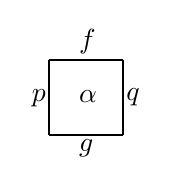
\begin{tikzpicture}[x=0.45pt,y=0.45pt,yscale=-1,xscale=1]
			%uncomment if require: \path (0,300); %set diagram left start at 0, and has height of 300
			
			%Straight Lines [id:da9493509620608491] 
			\draw    (40,40) -- (40,100) ;
			%Straight Lines [id:da8479191614730477] 
			\draw    (100,40) -- (100,100) ;
			%Straight Lines [id:da17087159934558604] 
			\draw    (40,40) -- (100,40) ;
			%Straight Lines [id:da17472272621664064] 
			\draw    (40,100) -- (100,100) ;
			
			% Text Node
			\draw (62,77) node [anchor=south west] [inner sep=0.75pt]   [align=left] {$\displaystyle \alpha$};
			% Text Node
			\draw (24,80) node [anchor=south west] [inner sep=0.75pt]   [align=left] {$\displaystyle p$};
			% Text Node
			\draw (100,79.17) node [anchor=south west] [inner sep=0.75pt]   [align=left] {$\displaystyle q$};
			% Text Node
			\draw (62,38) node [anchor=south west] [inner sep=0.75pt]   [align=left] {$\displaystyle f$};
			% Text Node
			\draw (62,120) node [anchor=south west] [inner sep=0.75pt]   [align=left] {$\displaystyle g$};
			
			
		\end{tikzpicture}
		$$
		若两个这样的同伦 $\alpha,\alpha'\colon I\times I\to X$ 相对于正方形的边界同伦, 则将其视为同一个 $2$-态射.
		\item 对每三个点 $p,q,r$, 复合 $\cdot\colon \operatorname{Hom}(q,r)\times \operatorname{Hom}(p,q)\to\operatorname{Hom}(p,r)$ 的定义为
		\[
		(f\cdot g)(t) = \begin{cases}
			g(2t) & 0\leq t \leq 1/2\\
			f(2t-1) & 1/2 < t \leq 1
		\end{cases}.
		\]
		这个复合不满足严格的结合律, 但存在如左下图显式的同伦 $\alpha\colon (f\cdot g)\cdot h \to f\cdot (g\cdot h)$.
		五边形公理体现为如右下图两个同伦之间的同伦.
		$$
		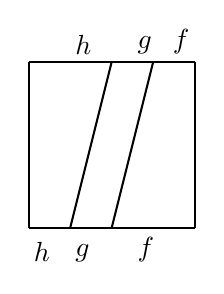
\begin{tikzpicture}[x=0.75pt,y=0.75pt,yscale=-1,xscale=1]
			%uncomment if require: \path (0,300); %set diagram left start at 0, and has height of 300
			
			%Straight Lines [id:da9493509620608491] 
			\draw    (40,40) -- (40,120) ;
			%Straight Lines [id:da8479191614730477] 
			\draw    (120,40) -- (120,120) ;
			%Straight Lines [id:da17087159934558604] 
			\draw    (40,40) -- (120,40) ;
			%Straight Lines [id:da17472272621664064] 
			\draw    (40,120) -- (120,120) ;
			%Straight Lines [id:da7159459773623977] 
			\draw    (80,40) -- (60,120) ;
			%Straight Lines [id:da7936546950580412] 
			\draw    (100,40) -- (80,120) ;
			
			% Text Node
			\draw (61,38) node [anchor=south west] [inner sep=0.75pt]   [align=left] {$\displaystyle h$};
			% Text Node
			\draw (108,38) node [anchor=south west] [inner sep=0.75pt]   [align=left] {$\displaystyle f$};
			% Text Node
			\draw (91,38) node [anchor=south west] [inner sep=0.75pt]   [align=left] {$\displaystyle g$};
			% Text Node
			\draw (41,138) node [anchor=south west] [inner sep=0.75pt]   [align=left] {$\displaystyle h$};
			% Text Node
			\draw (61,138) node [anchor=south west] [inner sep=0.75pt]   [align=left] {$\displaystyle g$};
			% Text Node
			\draw (91,138) node [anchor=south west] [inner sep=0.75pt]   [align=left] {$\displaystyle f$};
			
			
		\end{tikzpicture}
		\hspace{3em}
		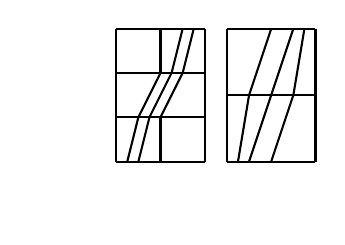
\begin{tikzpicture}[x=0.4pt,y=0.4pt,yscale=-1,xscale=1]
			\path (0,250); %set diagram left start at 0, and has height of 398
			
			%Straight Lines [id:da9493509620608491] 
			\draw    (80,160) -- (80,200) ;
			%Straight Lines [id:da8479191614730477] 
			\draw    (120,160) -- (120,200) ;
			%Straight Lines [id:da17087159934558604] 
			\draw    (80,160) -- (120,160) ;
			%Straight Lines [id:da17472272621664064] 
			\draw    (80,200) -- (120,200) ;
			%Straight Lines [id:da7159459773623977] 
			\draw    (100,160) -- (90,200) ;
			%Straight Lines [id:da7936546950580412] 
			\draw    (110,160) -- (100,200) ;
			%Straight Lines [id:da4333538566743742] 
			\draw    (120,160) -- (160,160) ;
			%Straight Lines [id:da2622244602659338] 
			\draw    (120,200) -- (160,200) ;
			%Straight Lines [id:da757640719712422] 
			\draw    (160,160) -- (160,200) ;
			%Straight Lines [id:da03544386120728049] 
			\draw    (80,120) -- (80,160) ;
			%Straight Lines [id:da7869492013227473] 
			\draw    (140,120) -- (120,160) ;
			%Straight Lines [id:da8440391323636871] 
			\draw    (160,120) -- (160,160) ;
			%Straight Lines [id:da7142265089887094] 
			\draw    (80,120) -- (120,120) ;
			%Straight Lines [id:da8471771371965053] 
			\draw    (120,120) -- (160,120) ;
			%Straight Lines [id:da0029227351176372984] 
			\draw    (120,120) -- (100,160) ;
			%Straight Lines [id:da5130194977669473] 
			\draw    (130,120) -- (110,160) ;
			%Straight Lines [id:da9722497425689605] 
			\draw    (120,80) -- (120,120) ;
			%Straight Lines [id:da5819252574569287] 
			\draw    (160,80) -- (160,120) ;
			%Straight Lines [id:da5253151554633011] 
			\draw    (140,80) -- (130,120) ;
			%Straight Lines [id:da3466940271955081] 
			\draw    (150,80) -- (140,120) ;
			%Straight Lines [id:da482698942279874] 
			\draw    (80,80) -- (80,120) ;
			%Straight Lines [id:da577335771369911] 
			\draw    (80,80) -- (120,80) ;
			%Straight Lines [id:da7062554999319648] 
			\draw    (120,80) -- (160,80) ;
			%Straight Lines [id:da7500750753354499] 
			\draw    (180,80) -- (220,80) ;
			%Straight Lines [id:da5909396267956115] 
			\draw    (220,80) -- (260,80) ;
			%Straight Lines [id:da6903461495201051] 
			\draw    (240,80) -- (220,140) ;
			%Straight Lines [id:da43860842476035544] 
			\draw    (220,80) -- (200,140) ;
			%Straight Lines [id:da8119236706978197] 
			\draw    (180,140) -- (220,140) ;
			%Straight Lines [id:da2477824013991532] 
			\draw    (220,140) -- (260,140) ;
			%Straight Lines [id:da10431419778749929] 
			\draw    (260,80) -- (260,140) ;
			%Straight Lines [id:da18509591125007274] 
			\draw    (180,80) -- (180,140) ;
			%Straight Lines [id:da21868267714023193] 
			\draw    (250,80) -- (240,140) ;
			%Straight Lines [id:da7712321706522733] 
			\draw    (260,200) -- (220,200) ;
			%Straight Lines [id:da7593643747347198] 
			\draw    (220,200) -- (180,200) ;
			%Straight Lines [id:da3540632371960386] 
			\draw    (200,200) -- (220,140) ;
			%Straight Lines [id:da0004735495623144903] 
			\draw    (220,200) -- (240,140) ;
			%Straight Lines [id:da9486324379201228] 
			\draw    (180,200) -- (180,140) ;
			%Straight Lines [id:da5967097776139811] 
			\draw    (260,200) -- (260,140) ;
			%Straight Lines [id:da7096217720274685] 
			\draw    (190,200) -- (200,140) ;
			
			
			
			
		\end{tikzpicture}
		$$
	\end{itemize}
	考虑点 $p$ 处的恒等态射, 即常值道路 $i_p$; 它到自身的 $2$-态射构成一个群, 即 $X$ 的第二阶同伦群 $\pi_2(X,p)$.
\end{example}

\begin{example}
	[label={locally-discrete-2-category}]
	{(局部离散 $2$-范畴)}
	一个普通范畴 $\mathcal C$ 可视为 $2$-范畴: 其态射范畴 $\operatorname{Hom}(A,B)$ 为离散范畴, 即 $2$-态射仅有恒等.
	称这样的 $2$-范畴为\emph{局部离散 $2$-范畴} (locally discrete $2$-category).
\end{example}

\begin{definition}
	{(对偶)}
	一个 $2$-范畴 $\mathcal C$ 不仅有一种 ``对偶'', 而是有三种:
	\begin{itemize}
		\item $\mathcal C^{\op}$, 反转 $1$-态射的方向;
		\item $\mathcal C^{\text{co}}$, 反转 $2$-态射的方向;
		\item $\mathcal C^{\text{co}\op}$, 同时反转 $1$-态射和 $2$-态射的方向.
	\end{itemize}
	%我们较常使用的是 $\mathcal C^{\op}$.
\end{definition}

\begin{definition}
	[label={2-functor}]
	{($2$-函子)}
	$2$-范畴之间一种合适的函子概念是 \emph{$2$-函子} (又称\emph{伪函子}, pseudofunctor\footnotemark{}), 它的定义是将严格 $2$-函子的定义中的等式改为自然同构.
	具体地, 对于 $2$-范畴 $\mathcal C,\mathcal D$,
	一个 $2$-函子 $F\colon \mathcal C\to\mathcal D$ 包含如下资料,
	\begin{itemize}
		\item 对 $\mathcal C$ 的每个对象 $A$, 有一个 $\mathcal D$ 的对象 $F(A)$;
		\item 对 $\mathcal C$ 的每两个对象 $A,B$, 有一个函子 $F_{A,B}\colon \operatorname{Hom}_{\mathcal C}(A,B) \to \operatorname{Hom}_{\mathcal D} (F(A),F(B))$;
		\item (\emph{保持态射的复合}) 对 $\mathcal C$ 的每三个对象 $A,B,C$, 有一个自然同构
		$$\gamma_{A,B,C}\colon F_{A,C}(-\circ -) \overset{\simeq}{\to} F_{B,C}(-)\circ F_{A,B}(-);$$
		\item (\emph{保持恒等态射}) 对 $\mathcal C$ 的每个对象 $A$, 有一个自然同构
		$$\iota_A\colon F_{A,A}\circ i_A \overset{\simeq}{\to} i_{F(A)}; $$
	\end{itemize}
	满足如下融贯性等式.
	\vspace{-5pt}%\footnotemark{}.
	% https://q.uiver.app/#q=WzAsNixbMCwxLCJGKGZcXGNpcmMgKGdcXGNpcmMgaCkpIl0sWzMsMCwiRihmXFxjaXJjIGcpXFxjaXJjIEYoaCkiXSxbMCwzLCJGKGYpXFxjaXJjIEYoZ1xcY2lyYyBoKSJdLFsyLDMsIkYoZilcXGNpcmMgKEYoZylcXGNpcmMgRihoKSkiXSxbMywyLCIoRihmKVxcY2lyYyBGKGcpKVxcY2lyYyBGKGgpIl0sWzEsMCwiRigoZlxcY2lyYyBnKVxcY2lyYyBoKSJdLFswLDIsIlxcZ2FtbWEiLDJdLFsyLDMsIlxcZ2FtbWEiLDIseyJzaG9ydGVuIjp7InRhcmdldCI6MzB9fV0sWzEsNCwiXFxnYW1tYSJdLFs1LDEsIlxcZ2FtbWEiLDAseyJzaG9ydGVuIjp7InNvdXJjZSI6MzB9fV0sWzUsMCwiXFxhbHBoYSIsMl0sWzQsMywiXFxhbHBoYSJdXQ==
	\[\begin{tikzcd}[ampersand replacement=\&,sep=tiny]
		\& {F((-\circ -)\circ -)\hspace{-3em}} \&\& {F(-\circ -)\circ F(-)} \\
		{F(-\circ (-\circ -))} \\
		\&\&\& {(F(-)\circ F(-))\circ F(-)} \\
		{F(-)\circ F(-\circ -)} \&\& {\hspace{-2em}F(-)\circ (F(-)\circ F(-))}
		\arrow["\gamma"', from=2-1, to=4-1]
		\arrow["\gamma"'{pos=0.3}, shorten >=22pt, from=4-1, to=4-3]
		\arrow["\gamma", from=1-4, to=3-4]
		\arrow["\gamma"{pos=0.7}, shorten <=32pt, from=1-2, to=1-4]
		\arrow["\alpha"', from=1-2, to=2-1]
		\arrow["\alpha", from=3-4, to=4-3]
	\end{tikzcd}\]
	% https://q.uiver.app/#q=WzAsNCxbMCwwLCJGKC0pXFxjaXJjIEYoaSkiXSxbMSwwLCJGKC0pXFxjaXJjIGkiXSxbMSwxLCJGKC0pIl0sWzAsMSwiRigtXFxjaXJjIGkpIl0sWzAsMSwiXFxpb3RhIl0sWzEsMiwiXFxyaG8iXSxbMywwLCJcXGdhbW1hIl0sWzMsMiwiXFxyaG8iLDJdXQ==
	\[\begin{tikzcd}[ampersand replacement=\&]
		{F(-)\circ F(i)} \& {F(-)\circ i} \\
		{F(-\circ i)} \& {F(-)}
		\arrow["\iota", from=1-1, to=1-2]
		\arrow["\rho", from=1-2, to=2-2]
		\arrow["\gamma", from=2-1, to=1-1]
		\arrow["\rho"', from=2-1, to=2-2]
	\end{tikzcd}\]
\end{definition}
%\addtocounter{footnote}{-1}
\footnotetext{注意我们所说的 $2$-范畴均为弱 $2$-范畴. 此外有若干种不同的 $2$-函子的概念, 但 ``伪函子'' 这个名字不好听, 故以 $2$-函子称呼这种概念.}
%\addtocounter{footnote}{1}
%\footnotetext{图中省略了 $\circ$ 的结合子.}

\begin{example}
	{(Hom 函子)}
	对于 $2$-范畴 $\mathcal C$ 中的对象 $X$, 有 $2$-函子 $\operatorname{Hom}_{\mathcal C}(X,-)\colon \mathcal C\to\mathcal Cat$.
	\begin{itemize}
		\item 在对象层面, $\operatorname{Hom}_{\mathcal C}(X,A)$ 即 $\mathcal C$ 本身的资料;
		\item 对两个对象 $A,B$, 函子 $\operatorname{Hom}_{\mathcal C}(A,B)\to\operatorname{Hom}_{\mathcal Cat}\big({\operatorname{Hom}(X,A),\operatorname{Hom}(X,B)}\big)$ 来自于复合函子 $\circ\colon \operatorname{Hom}_{\mathcal C}(A,B)\times \operatorname{Hom}_{\mathcal C}(X,A) \to \operatorname{Hom}_{\mathcal C}(X,B)$;
		\item $2$-函子的定义中其它结构和性质皆出自 $2$-范畴 $\mathcal C$ 的结构和性质.
	\end{itemize}
	类似地, 有 $2$-函子 $\operatorname{Hom}_{\mathcal C}(-,X)\colon \mathcal C^{\op}\to \mathcal Cat$.
\end{example}

\subsection{$2$-范畴中的万有性质}

\begin{propdef}
	[label={terminal-object-2-category}]
	{($2$-范畴的终对象)}
	设 $\mathcal C$ 为 $2$-范畴, 称 $\mathcal C$ 的对象 $1$ 为\emph{终对象}是指对任何对象 $X$,
	$\operatorname{Hom}(X,1)$ 等价于终范畴.
	展开所有定义, 这意味着对任何对象 $X$ 存在 $1$-态射 $X\to 1$,
	且对任何两个 $1$-态射 $f,g\colon X\to 1$, 存在唯一的 $2$-态射 $\alpha\colon f\to g$,
	且 $\alpha$ 为同构.
	
	与普通范畴中类似, 终对象 (乃至一般的极限) 可定义为函子 $\mathcal C^{\op}\to\mathcal Cat$ 的表示对象.
\end{propdef}

\subsection{俯 $2$-范畴}

\begin{definition}
	{(俯 $2$-范畴)}
	设 $\mathcal C$ 为 $2$-范畴, $X$ 为其对象. 定义\emph{俯 $2$-范畴} $\mathcal C/X$ 如下,
	\begin{itemize}
		\item 对象为 $\mathcal C$ 中的态射 $Y\to X$;
		\item 态射为 (差一个 $2$-同构的) 交换图% https://q.uiver.app/#q=WzAsMyxbMCwwLCJZIl0sWzEsMSwiWCJdLFsyLDAsIloiXSxbMCwxXSxbMCwyXSxbMiwxXSxbMywyLCJcXHNpbWVxIiwxLHsibGFiZWxfcG9zaXRpb24iOjQwLCJvZmZzZXQiOjEsInNob3J0ZW4iOnsic291cmNlIjoyMCwidGFyZ2V0IjozMH19XV0=
		\[\begin{tikzcd}[ampersand replacement=\&,column sep=small]
			Y \&\& Z; \\
			\& X
			\arrow[""{name=0, anchor=center, inner sep=0}, from=1-1, to=2-2]
			\arrow[from=1-1, to=1-3]
			\arrow[from=1-3, to=2-2]
			\arrow["\simeq"{description, pos=0.4}, shift right, shorten <=8pt, shorten >=12pt, Rightarrow, from=0, to=1-3]
		\end{tikzcd}\]
		\item $2$-态射为如下的图.
		% https://q.uiver.app/#q=WzAsMyxbMCwwLCJZIl0sWzEsMSwiWCJdLFsyLDAsIloiXSxbMCwxXSxbMCwyLCIiLDIseyJjdXJ2ZSI6LTF9XSxbMiwxXSxbMCwyLCIiLDIseyJjdXJ2ZSI6MX1dLFszLDIsIlxcc2ltZXEiLDEseyJsYWJlbF9wb3NpdGlvbiI6NDAsIm9mZnNldCI6MSwic2hvcnRlbiI6eyJzb3VyY2UiOjIwLCJ0YXJnZXQiOjMwfX1dLFs2LDQsIiIsMCx7InNob3J0ZW4iOnsic291cmNlIjoyMCwidGFyZ2V0IjoyMH19XV0=
		\[\begin{tikzcd}[ampersand replacement=\&,column sep=small]
			Y \&\& Z \\
			\& X
			\arrow[""{name=0, anchor=center, inner sep=0}, from=1-1, to=2-2]
			\arrow[""{name=1, anchor=center, inner sep=0}, bend left=15, from=1-1, to=1-3]
			\arrow[from=1-3, to=2-2]
			\arrow[""{name=2, anchor=center, inner sep=0}, bend right=15, from=1-1, to=1-3]
			\arrow["\simeq"{description, pos=0.4}, shift right, shorten <=8pt, shorten >=12pt, Rightarrow, from=0, to=1-3]
			\arrow[shorten <=2pt, shorten >=2pt, Rightarrow, from=2, to=1]
		\end{tikzcd}\]
	\end{itemize}
\end{definition}

\section{伴随}

$2$-范畴是谈论伴随的自然的语境.

\newcommand{\adj}[4]{
\begin{tikzcd}[ampersand replacement=\&]
	{#3} \& {#4}
	\arrow[""{name=0, anchor=center, inner sep=0}, "#1"', shift right=2, from=1-2, to=1-1]
	\arrow[""{name=1, anchor=center, inner sep=0}, "#2"', shift right=2, from=1-1, to=1-2]
	\arrow["\dashv"{anchor=center, rotate=-90}, draw=none, from=0, to=1]
\end{tikzcd}
}

\begin{definition}
	[label={adjoints-in-2-categories}]
	{(伴随)}
	一个 $2$-范畴中的一组\emph{伴随} $\adj{F}{G}{D}{C}$ 是如下资料:
	\begin{itemize}
		\item 两个对象 $C,D$,
		\item 两个态射 $F\colon C\to D$ (称为\emph{左伴随}), $G\colon D\to C$ (称为\emph{右伴随}),
		\item 两个 $2$-态射 $\eta\colon \operatorname{id}_C\to GF$ (称为\emph{单位}), $\varepsilon\colon FG\to\operatorname{id}_D$ (称为\emph{余单位});
	\end{itemize}
	满足如下 $2$-态射的等式,
	\[\begin{tikzcd}[ampersand replacement=\&,column sep=1.5em]
		{C} \&\& {C} \\
		\& {D} \&\& {D}
		\arrow["F"', from=1-1, to=2-2]
		\arrow["G"{description}, from=2-2, to=1-3]
		\arrow["F", from=1-3, to=2-4]
		\arrow[""{name=0, anchor=center, inner sep=0}, "{\operatorname{id}_{\mathcal C}}", from=1-1, to=1-3]
		\arrow[""{name=1, anchor=center, inner sep=0}, "{\operatorname{id}_{\mathcal D}}"', from=2-2, to=2-4]
		\arrow["\eta"', shorten <=3pt, shorten >=3pt, Rightarrow, from=0, to=2-2]
		\arrow["\varepsilon", shorten <=3pt, shorten >=3pt, Rightarrow, from=1-3, to=1]
	\end{tikzcd}\hspace{-1em}=\operatorname{id}_F,
	\begin{tikzcd}[ampersand replacement=\&,column sep=1.5em]
		\& {C} \&\& {C} \\
		{D} \&\& {D}
		\arrow["G", from=2-1, to=1-2]
		\arrow["F"{description}, from=1-2, to=2-3]
		\arrow["G"', from=2-3, to=1-4]
		\arrow[""{name=0, anchor=center, inner sep=0}, "{\operatorname{id}_{\mathcal D}}"', from=2-1, to=2-3]
		\arrow[""{name=1, anchor=center, inner sep=0}, "{\operatorname{id}_{\mathcal C}}", from=1-2, to=1-4]
		\arrow["\varepsilon", shorten <=3pt, shorten >=3pt, Rightarrow, from=1-2, to=0]
		\arrow["\eta"', shorten <=3pt, shorten >=3pt, Rightarrow, from=1, to=2-3]
	\end{tikzcd}\hspace{-1em}=\operatorname{id}_{G}.\]

	这个条件也可用线图\footnotemark{}表示为

\tikzset{every picture/.style={line width=0.75pt}} %set default line width to 0.75pt        
\begin{center}
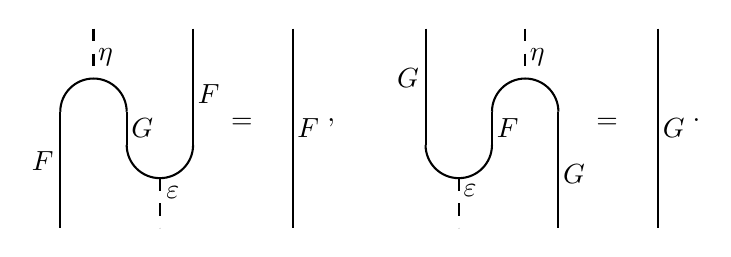
\begin{tikzpicture}[x=0.75pt,y=0.75pt,yscale=-0.8,xscale=0.8]
	%uncomment if require: \path (0,300); %set diagram left start at 0, and has height of 300
	
	%Straight Lines [id:da4698218774091225] 
	\draw    (100,130) -- (100,200) ;
	%Shape: Arc [id:dp5452146741155406] 
	\draw  [draw opacity=0] (100,130) .. controls (100,118.95) and (108.95,110) .. (120,110) .. controls (131.05,110) and (140,118.95) .. (140,130) -- (120,130) -- cycle ; \draw   (100,130) .. controls (100,118.95) and (108.95,110) .. (120,110) .. controls (131.05,110) and (140,118.95) .. (140,130) ;  
	%Shape: Arc [id:dp49645291516622003] 
	\draw  [draw opacity=0] (180,150) .. controls (180,150) and (180,150) .. (180,150) .. controls (180,150) and (180,150) .. (180,150) .. controls (180,161.05) and (171.05,170) .. (160,170) .. controls (148.95,170) and (140,161.05) .. (140,150) -- (160,150) -- cycle ; \draw   (180,150) .. controls (180,150) and (180,150) .. (180,150) .. controls (180,150) and (180,150) .. (180,150) .. controls (180,161.05) and (171.05,170) .. (160,170) .. controls (148.95,170) and (140,161.05) .. (140,150) ;  
	%Straight Lines [id:da07095399149030768] 
	\draw    (180,80) -- (180,150) ;
	%Straight Lines [id:da08445793804465951] 
	\draw  [dash pattern={on 4.5pt off 4.5pt}]  (120,80) -- (120,110) ;
	%Straight Lines [id:da40802862615686375] 
	\draw  [dash pattern={on 4.5pt off 4.5pt}]  (160,170) -- (160,200) ;
	%Straight Lines [id:da5905893191283564] 
	\draw    (140,130) -- (140,150) ;
	%Straight Lines [id:da7172863956237474] 
	\draw    (240,80) -- (240,200) ;
	%Straight Lines [id:da6534130406395566] 
	\draw    (320,80) -- (320,150) ;
	%Shape: Arc [id:dp37941315902148687] 
	\draw  [draw opacity=0] (360,130) .. controls (360,118.95) and (368.95,110) .. (380,110) .. controls (391.05,110) and (400,118.95) .. (400,130) -- (380,130) -- cycle ; \draw   (360,130) .. controls (360,118.95) and (368.95,110) .. (380,110) .. controls (391.05,110) and (400,118.95) .. (400,130) ;  
	%Shape: Arc [id:dp314690779386831] 
	\draw  [draw opacity=0] (360,150) .. controls (360,150) and (360,150) .. (360,150) .. controls (360,150) and (360,150) .. (360,150) .. controls (360,161.05) and (351.05,170) .. (340,170) .. controls (328.95,170) and (320,161.05) .. (320,150) -- (340,150) -- cycle ; \draw   (360,150) .. controls (360,150) and (360,150) .. (360,150) .. controls (360,150) and (360,150) .. (360,150) .. controls (360,161.05) and (351.05,170) .. (340,170) .. controls (328.95,170) and (320,161.05) .. (320,150) ;  
	%Straight Lines [id:da0821788481682626] 
	\draw    (400,130) -- (400,200) ;
	%Straight Lines [id:da026745112319709996] 
	\draw  [dash pattern={on 4.5pt off 4.5pt}]  (380,80) -- (380,110) ;
	%Straight Lines [id:da08383119415628326] 
	\draw  [dash pattern={on 4.5pt off 4.5pt}]  (340,170) -- (340,200) ;
	%Straight Lines [id:da867238855772305] 
	\draw    (360,130) -- (360,150) ;
	%Straight Lines [id:da7093402738130186] 
	\draw    (460,80) -- (460,200) ;
	
	% Text Node
	\draw (81,152) node [anchor=north west][inner sep=0.75pt]   [align=left] {$\displaystyle F$};
	% Text Node
	\draw (141,132) node [anchor=north west][inner sep=0.75pt]   [align=left] {$\displaystyle G$};
	% Text Node
	\draw (181,112) node [anchor=north west][inner sep=0.75pt]   [align=left] {$\displaystyle F$};
	% Text Node
	\draw (201,132) node [anchor=north west][inner sep=0.75pt]   [align=left] {$\displaystyle =$};
	% Text Node
	\draw (241,132) node [anchor=north west][inner sep=0.75pt]   [align=left] {$\displaystyle F$};
	% Text Node
	\draw (301,102) node [anchor=north west][inner sep=0.75pt]   [align=left] {$\displaystyle G$};
	% Text Node
	\draw (361,132) node [anchor=north west][inner sep=0.75pt]   [align=left] {$\displaystyle F$};
	% Text Node
	\draw (421,132) node [anchor=north west][inner sep=0.75pt]   [align=left] {$\displaystyle =$};
	% Text Node
	\draw (461,132) node [anchor=north west][inner sep=0.75pt]   [align=left] {$\displaystyle G$};
	% Text Node
	\draw (401,160) node [anchor=north west][inner sep=0.75pt]   [align=left] {$\displaystyle G$};
	% Text Node
	\draw (259,132) node [anchor=north west][inner sep=0.75pt]   [align=left] {$\displaystyle ,$};
	% Text Node
	\draw (479,132) node [anchor=north west][inner sep=0.75pt]   [align=left] {$\displaystyle .$};
	% Text Node
	\draw (121,90) node [anchor=north west][inner sep=0.75pt]   [align=left] {$\displaystyle \eta $};
	% Text Node
	\draw (162,173) node [anchor=north west][inner sep=0.75pt]   [align=left] {$\displaystyle \varepsilon $};
	% Text Node
	\draw (341,172) node [anchor=north west][inner sep=0.75pt]   [align=left] {$\displaystyle \varepsilon $};
	% Text Node
	\draw (381,90) node [anchor=north west][inner sep=0.75pt]   [align=left] {$\displaystyle \eta $};
	
	
\end{tikzpicture}
\end{center}

\end{definition}
\footnotetext{线图是表示一些 $2$-范畴结构的工具. 在一个图中, 平面区域表示 $2$-范畴的对象, 平面区域之间的分界线表示 $1$-态射, 分界线上的分段点表示 $2$-态射.}
\begin{example}
	{(伴随函子)}
	$2$-范畴 $\mathcal {C}at$ 中的伴随就是熟知的伴随函子. 对于伴随函子 $F\colon \mathcal C\to\mathcal D$, $G\colon \mathcal D\to\mathcal C$, 如下的线图给出了映射
	$$
	\operatorname{Hom}(Fc,d) \to \operatorname{Hom}(c,Gd).
	$$
	\begin{center}
		
		
		\tikzset{every picture/.style={line width=0.75pt}} %set default line width to 0.75pt        
		
		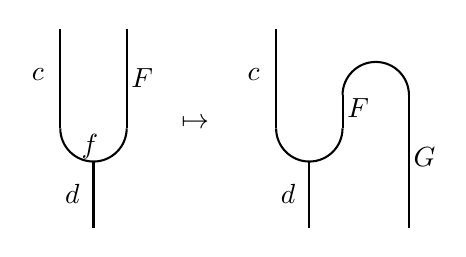
\begin{tikzpicture}[x=0.75pt,y=0.75pt,yscale=-0.8,xscale=0.8]
			%uncomment if require: \path (0,300); %set diagram left start at 0, and has height of 300
			
			%Straight Lines [id:da38389280296337147] 
			\draw    (70,100) -- (70,160) ;
			%Shape: Arc [id:dp500451274224406] 
			\draw  [draw opacity=0] (110,160) .. controls (110,160) and (110,160) .. (110,160) .. controls (110,160) and (110,160) .. (110,160) .. controls (110,171.05) and (101.05,180) .. (90,180) .. controls (78.95,180) and (70,171.05) .. (70,160) -- (90,160) -- cycle ; \draw   (110,160) .. controls (110,160) and (110,160) .. (110,160) .. controls (110,160) and (110,160) .. (110,160) .. controls (110,171.05) and (101.05,180) .. (90,180) .. controls (78.95,180) and (70,171.05) .. (70,160) ;  
			%Straight Lines [id:da36761146974596803] 
			\draw    (110,100) -- (110,160) ;
			%Straight Lines [id:da28528438514767007] 
			\draw    (90,180) -- (90,220) ;
			%Straight Lines [id:da2956003592318719] 
			\draw    (200,100) -- (200,160) ;
			%Shape: Arc [id:dp007579126105482503] 
			\draw  [draw opacity=0] (240,160) .. controls (240,160) and (240,160) .. (240,160) .. controls (240,160) and (240,160) .. (240,160) .. controls (240,171.05) and (231.05,180) .. (220,180) .. controls (208.95,180) and (200,171.05) .. (200,160) -- (220,160) -- cycle ; \draw   (240,160) .. controls (240,160) and (240,160) .. (240,160) .. controls (240,160) and (240,160) .. (240,160) .. controls (240,171.05) and (231.05,180) .. (220,180) .. controls (208.95,180) and (200,171.05) .. (200,160) ;  
			%Straight Lines [id:da48802759810410334] 
			\draw    (240,140) -- (240,160) ;
			%Straight Lines [id:da20597425552353443] 
			\draw    (220,180) -- (220,220) ;
			%Shape: Arc [id:dp2471225279229352] 
			\draw  [draw opacity=0] (240,140) .. controls (240,128.95) and (248.95,120) .. (260,120) .. controls (271.05,120) and (280,128.95) .. (280,140) -- (260,140) -- cycle ; \draw   (240,140) .. controls (240,128.95) and (248.95,120) .. (260,120) .. controls (271.05,120) and (280,128.95) .. (280,140) ;  
			%Straight Lines [id:da42525487208205326] 
			\draw    (280,140) -- (280,220) ;
			
			% Text Node
			\draw (141,152) node [anchor=north west][inner sep=0.75pt]   [align=left] {$\displaystyle \mapsto$};
			% Text Node
			\draw (51,122) node [anchor=north west][inner sep=0.75pt]   [align=left] {$\displaystyle c$};
			% Text Node
			\draw (111,122) node [anchor=north west][inner sep=0.75pt]   [align=left] {$\displaystyle F$};
			% Text Node
			\draw (71,192) node [anchor=north west][inner sep=0.75pt]   [align=left] {$\displaystyle d$};
			% Text Node
			\draw (81,162) node [anchor=north west][inner sep=0.75pt]   [align=left] {$\displaystyle f$};
			% Text Node
			\draw (181,122) node [anchor=north west][inner sep=0.75pt]   [align=left] {$\displaystyle c$};
			% Text Node
			\draw (241,140) node [anchor=north west][inner sep=0.75pt]   [align=left] {$\displaystyle F$};
			% Text Node
			\draw (281,170) node [anchor=north west][inner sep=0.75pt]   [align=left] {$\displaystyle G$};
			% Text Node
			\draw (201,192) node [anchor=north west][inner sep=0.75pt]   [align=left] {$\displaystyle d$};
			
		\end{tikzpicture}
	\end{center}
	其中我们将对象 $c$ 视为函子 $1\to\mathcal C$. 考虑一个形如
	\tikzset{every picture/.style={line width=0.75pt}} %set default line width to 0.75pt        
	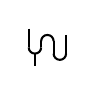
\begin{tikzpicture}[x=0.75pt,y=0.75pt,yscale=-0.15,xscale=0.15]
		%uncomment if require: \path (0,300); %set diagram left start at 0, and has height of 300
		
		%Straight Lines [id:da9426120658362054] 
		\draw    (200,100) -- (200,160) ;
		%Shape: Arc [id:dp7574128344072426] 
		\draw  [draw opacity=0] (240,160) .. controls (240,160) and (240,160) .. (240,160) .. controls (240,160) and (240,160) .. (240,160) .. controls (240,171.05) and (231.05,180) .. (220,180) .. controls (208.95,180) and (200,171.05) .. (200,160) -- (220,160) -- cycle ; \draw   (240,160) .. controls (240,160) and (240,160) .. (240,160) .. controls (240,160) and (240,160) .. (240,160) .. controls (240,171.05) and (231.05,180) .. (220,180) .. controls (208.95,180) and (200,171.05) .. (200,160) ;  
		%Straight Lines [id:da6440236067654423] 
		\draw    (240,140) -- (240,160) ;
		%Straight Lines [id:da6278109278126796] 
		\draw    (220,180) -- (220,220) ;
		%Shape: Arc [id:dp5036962649695886] 
		\draw  [draw opacity=0] (240,140) .. controls (240,128.95) and (248.95,120) .. (260,120) .. controls (271.05,120) and (280,128.95) .. (280,140) -- (260,140) -- cycle ; \draw   (240,140) .. controls (240,128.95) and (248.95,120) .. (260,120) .. controls (271.05,120) and (280,128.95) .. (280,140) ;  
		%Straight Lines [id:da8724403377021124] 
		\draw    (280,140) -- (280,180) ;
		%Shape: Arc [id:dp2997750340889149] 
		\draw  [draw opacity=0] (320,180) .. controls (320,180) and (320,180) .. (320,180) .. controls (320,180) and (320,180) .. (320,180) .. controls (320,191.05) and (311.05,200) .. (300,200) .. controls (288.95,200) and (280,191.05) .. (280,180) -- (300,180) -- cycle ; \draw   (320,180) .. controls (320,180) and (320,180) .. (320,180) .. controls (320,180) and (320,180) .. (320,180) .. controls (320,191.05) and (311.05,200) .. (300,200) .. controls (288.95,200) and (280,191.05) .. (280,180) ;  
		%Straight Lines [id:da9641461547001391] 
		\draw    (320,120) -- (320,180) ;
	\end{tikzpicture}
	的线图, 我们得到上述映射为同构. 更一般地, 两对伴随给出的如下对应为同构, 有人称为 ``\emph{搭档}'' (mates).
	%\tikzset{every picture/.style={line width=0.75pt}} %set default line width to 0.75pt        
	\[
	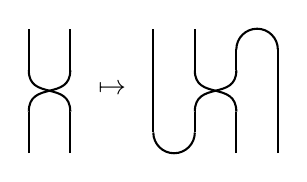
\begin{tikzpicture}[x=0.75pt,y=0.75pt,yscale=-0.5,xscale=0.5]
		%uncomment if require: \path (0,300); %set diagram left start at 0, and has height of 300
		
		%Straight Lines [id:da6760491461500817] 
		\draw    (60,110) -- (60,70) ;
		%Straight Lines [id:da10042447386234477] 
		\draw    (100,110) -- (100,70) ;
		%Straight Lines [id:da47368418503953036] 
		\draw    (60,190) -- (60,150) ;
		%Straight Lines [id:da4294561706343043] 
		\draw    (100,190) -- (100,150) ;
		%Straight Lines [id:da08550817636137276] 
		\draw    (220,110) -- (220,70) ;
		%Straight Lines [id:da7093862650682823] 
		\draw    (260,110) -- (260,90) ;
		%Straight Lines [id:da11766526028546886] 
		\draw    (220,170) -- (220,150) ;
		%Straight Lines [id:da5510776222620308] 
		\draw    (260,190) -- (260,150) ;
		%Shape: Arc [id:dp697920581597592] 
		\draw  [draw opacity=0] (220,170) .. controls (220,170) and (220,170) .. (220,170) .. controls (220,170) and (220,170) .. (220,170) .. controls (220,181.05) and (211.05,190) .. (200,190) .. controls (188.95,190) and (180,181.05) .. (180,170) -- (200,170) -- cycle ; \draw   (220,170) .. controls (220,170) and (220,170) .. (220,170) .. controls (220,170) and (220,170) .. (220,170) .. controls (220,181.05) and (211.05,190) .. (200,190) .. controls (188.95,190) and (180,181.05) .. (180,170) ;  
		%Shape: Arc [id:dp3549910728085319] 
		\draw  [draw opacity=0] (300,90) .. controls (300,90) and (300,90) .. (300,90) .. controls (300,90) and (300,90) .. (300,90) .. controls (300,78.95) and (291.05,70) .. (280,70) .. controls (268.95,70) and (260,78.95) .. (260,90) -- (280,90) -- cycle ; \draw   (300,90) .. controls (300,90) and (300,90) .. (300,90) .. controls (300,90) and (300,90) .. (300,90) .. controls (300,78.95) and (291.05,70) .. (280,70) .. controls (268.95,70) and (260,78.95) .. (260,90) ;  
		%Straight Lines [id:da6613547275597564] 
		\draw    (180,170) -- (180,70) ;
		%Straight Lines [id:da5281322189812798] 
		\draw    (300,190) -- (300,90) ;
		%Curve Lines [id:da6896703183364732] 
		\draw    (60,110) .. controls (59.94,139.56) and (99.94,119.81) .. (100,150) ;
		%Curve Lines [id:da8710144571035341] 
		\draw    (100,110) .. controls (99.94,139.56) and (59.94,119.81) .. (60,150) ;
		%Curve Lines [id:da7905113406699873] 
		\draw    (220,110) .. controls (219.94,139.56) and (259.94,119.81) .. (260,150) ;
		%Curve Lines [id:da7196754149364168] 
		\draw    (260,110) .. controls (259.94,139.56) and (219.94,119.81) .. (220,150) ;
		
		% Text Node
		\draw (124,121) node [anchor=north west][inner sep=0.75pt]   [align=left] {$\displaystyle \mapsto $};
	\end{tikzpicture}
	\]
\end{example}

\begin{example}
	[label={terminal-object-2-categorical}]
	{(终点)}
	设一个 $2$-范畴 $\mathcal C$ 有终对象 $1$.
	对于 $\mathcal C$ 的对象 $X$, 若 $1$-态射 $X\to 1$ 有右伴随, 则称 $X$ 有\emph{终点}.
	例如 $2$-范畴 $\mathcal {C}at$ 的一个对象有终点就是说它有终对象. 因此, 表达 ``范畴的终对象'' 可使用 $\mathcal {C}at$ 中纯粹 $2$-范畴的语言, 而无需 ``拆开'' 这个范畴本身的结构.
\end{example}

\begin{propdef}
	[label={walking-adjunction}]
	{(游走的伴随)}
	如下定义一个 $2$-范畴 $\mathsf {Adj}$, 其中
	\begin{itemize}
		\item 有两个对象 $C,D$;
		\item 态射由两个态射 $F\colon C\to D$, $G\colon D\to C$ 自由生成;
		\item $2$-态射由 $\eta\colon \operatorname{id}_C\to GF$, $\varepsilon\colon FG\to\operatorname{id}_D$ 在定义 \ref{adjoints-in-2-categories} 中的关系下自由生成.
	\end{itemize}
	那么 $\mathsf {Adj}$ 是\emph{游走的伴随} (walking adjunction), 即任何 $2$-范畴 $\mathcal X$ 中的一对伴随等同于一个 $2$-函子 $\mathsf {Adj} \to \mathcal X$.
	稍具体一些, $\mathsf {Adj}$ 中的态射范畴可表示如下.
	\begin{itemize}
		\item
		$\operatorname{Hom}(C,C) = \begin{tikzcd}[ampersand replacement=\&,sep=small]
			{\operatorname{id}_C} \& GF \& GFGF \& \cdots
			\arrow["\eta", from=1-1, to=1-2]
			\arrow[shift left=2, from=1-2, to=1-3]
			\arrow[shift right=2, from=1-2, to=1-3]
			\arrow[from=1-3, to=1-2]
			\arrow[from=1-3, to=1-4]
			\arrow[shift left=4, from=1-3, to=1-4]
			\arrow[shift right=4, from=1-3, to=1-4]
			\arrow[shift left=2, from=1-4, to=1-3]
			\arrow[shift right=2, from=1-4, to=1-3]
		\end{tikzcd}$.
		记 $\Delta_+$ 为有限全序集 $[-1],[0],[1],[2],\cdots$ 与保序映射构成的范畴 (其中 $[n]=\{0,1,\cdots,n\}$, $[-1]=\varnothing$), 则 $\operatorname{Hom}(C,C)\simeq\Delta_+$. $\Delta_+$ 是所谓\emph{增广单纯形范畴} (augmented simplex category), 即单纯形范畴 $\Delta$ 添加一个始对象 $[-1]$.
		\item
		$\operatorname{Hom}(C,D) = \begin{tikzcd}[ampersand replacement=\&,sep=small]
			F \& FGF \& FGFGF \& \cdots
			\arrow["\eta", shift left, from=1-1, to=1-2]
			\arrow["\varepsilon", shift left, from=1-2, to=1-1]
			\arrow[shift right, from=1-2, to=1-3]
			\arrow[shift left=3, from=1-2, to=1-3]
			\arrow[shift right, from=1-3, to=1-2]
			\arrow[shift left=3, from=1-3, to=1-2]
			\arrow[shift left=5, from=1-3, to=1-4]
			\arrow[shift left, from=1-3, to=1-4]
			\arrow[shift right=3, from=1-3, to=1-4]
			\arrow[shift right=3, from=1-4, to=1-3]
			\arrow[shift left, from=1-4, to=1-3]
			\arrow[shift left=5, from=1-4, to=1-3]
		\end{tikzcd}$.
		记 $\Delta_{\bot}$ 为 $\Delta$ 的对象 $[0],[1],[2],\cdots$ 以及其中\emph{保持最小元的映射}构成的子范畴.
		则 $\operatorname{Hom}(C,D) \simeq\Delta_{\bot}$.
		\item $\operatorname{Hom}(D,D)\simeq\operatorname{Hom}(C,C)^{\op}$, $\operatorname{Hom}(D,C)\simeq\operatorname{Hom}(C,D)^{\op}$.
	\end{itemize}
\end{propdef}

\subsection{伴随保持极限}

现在我们谈论范畴之间的伴随函子.

\begin{prop}
	[label={adjoints-preserve-limits}]
	{}
	右伴随保持极限, 左伴随保持余极限.
\end{prop}

\begin{proof}
	由对偶性, 我们仅须证明前一个命题, 即右伴随保持极限. 设有伴随
	$\begin{tikzcd}[ampersand replacement=\&]
		{\mathcal {D}} \& {\mathcal {C},}
		\arrow[""{name=0, anchor=center, inner sep=0}, "F"', shift right=2, from=1-2, to=1-1]
		\arrow[""{name=1, anchor=center, inner sep=0}, "G"', shift right=2, from=1-1, to=1-2]
		\arrow["\dashv"{anchor=center, rotate=-90}, draw=none, from=0, to=1]
	\end{tikzcd}$
	设 $X \colon I \to \mathcal D$ 是任意图表 ($I$ 是小范畴).
	若极限 $\lim_i X_i$ 存在,
	则有自然同构
	\begin{align*}
		\operatorname{Hom}_{\mathcal C}(-,G\lim_i X_i)
		&\simeq \operatorname{Hom}_{\mathcal D}(F-,\lim_i X_i)&(1)\\
		&\simeq \lim_i \operatorname{Hom}_{\mathcal D}(F-,X_i)&(2)\\
		&\simeq \lim_i \operatorname{Hom}_{\mathcal C}(-,GX_i)&(3)\\
		&\simeq \operatorname{Hom}_{\mathcal C}(-,\lim_i GX_i).&(4)
	\end{align*}
	由米田引理, 得同构 $G\lim_i X_i \simeq \lim_i GX_i$,
	故右伴随保持极限\footnotemark{}.
	该证明可总结于下图中:
	% https://q.uiver.app/#q=WzAsOCxbMCwxLCJcXG1hdGhjYWwgQyJdLFsyLDEsIlxcbWF0aGNhbCBEIl0sWzAsMywiXFxtYXRoY2FsIENeSSJdLFsyLDMsIlxcbWF0aGNhbCBEXkkiXSxbMSwwLCJcXHdpZGVoYXQge1xcbWF0aGNhbCBDfSJdLFszLDAsIlxcd2lkZWhhdCB7XFxtYXRoY2FsIER9Il0sWzEsMiwiKFxcd2lkZWhhdCB7XFxtYXRoY2FsIEN9KV5JIl0sWzMsMiwiKFxcd2lkZWhhdCB7XFxtYXRoY2FsIER9KV5JIl0sWzEsMCwiRyIsMix7ImxhYmVsX3Bvc2l0aW9uIjozMH1dLFszLDIsIkdeSSIsMCx7ImxhYmVsX3Bvc2l0aW9uIjozMH1dLFswLDQsIlxceW8iXSxbMSw1LCJcXHlvIiwyXSxbMywxLCJcXG9wZXJhdG9ybmFtZXtsaW19IiwyLHsibGFiZWxfcG9zaXRpb24iOjMwfV0sWzIsMCwiXFxvcGVyYXRvcm5hbWV7bGltfSIsMCx7ImxhYmVsX3Bvc2l0aW9uIjozMH1dLFs3LDUsIlxcb3BlcmF0b3JuYW1le2xpbX0iLDIseyJsYWJlbF9wb3NpdGlvbiI6MzB9XSxbNiw0LCJcXG9wZXJhdG9ybmFtZXtsaW19IiwwLHsibGFiZWxfcG9zaXRpb24iOjMwfV0sWzIsNiwie1xceW99XkkiLDJdLFszLDcsIntcXHlvfV5JIiwyXSxbNSw0LCJGXioiLDIseyJsYWJlbF9wb3NpdGlvbiI6NzB9XSxbNyw2LCJGXioiLDAseyJsYWJlbF9wb3NpdGlvbiI6NzB9XV0= 
	\[\begin{tikzcd}[ampersand replacement=\&] \& {\widehat {\mathcal C}} \&\& {\widehat {\mathcal D}} \\ {\mathcal C} \&\& {\mathcal D} \\ \& {(\widehat {\mathcal C})^I} \&\& {(\widehat {\mathcal D})^I} \\ {\mathcal C^I} \&\& {\mathcal D^I} \arrow["{F^*}"'{pos=0.7}, from=1-4, to=1-2] \arrow["\yo", from=2-1, to=1-2] \arrow["\yo"', from=2-3, to=1-4] \arrow["G"'{pos=0.3}, from=2-3, to=2-1] \arrow["{\operatorname{lim}}"{pos=0.3}, from=3-2, to=1-2] \arrow["{\operatorname{lim}}"'{pos=0.3}, from=3-4, to=1-4] \arrow["{F^*}"{pos=0.7}, from=3-4, to=3-2] \arrow["{\operatorname{lim}}"{pos=0.3}, from=4-1, to=2-1] \arrow["{{\yo}^I}"', from=4-1, to=3-2] \arrow["{\operatorname{lim}}"'{pos=0.3}, from=4-3, to=2-3] \arrow["{{\yo}^I}"', from=4-3, to=3-4] \arrow["{G^I}"{pos=0.3}, from=4-3, to=4-1] \end{tikzcd}\]
	正方体的左右两面 (``米田嵌入保持极限'') 用在 (2), (4) 两处; 上下两面表达了 $F$ 是 $G$ 的左伴随, 用在 (1), (3) 两处; ``后'' 面 ($F^*$ 和 $F^*$ 所在的方块)
	%即如下的命题: 对 $\mathcal D$ 上的一族预层 $X\colon I\to\widetilde {\mathcal D}$,
	%\[
	%\operatorname{lim}^{\widehat {\mathcal C}}_i F^*X_i \simeq F^*\operatorname{lim}^{\widehat {\mathcal D}}_i X_i,
	%\]
	是由于 ``预层的极限逐点计算''.
	由于米田嵌入是全忠实函子, 我们得到正方体的 ``前'' 面 ($G$ 和 $G^I$ 所在的方块) 交换, 而这正是要证的结论.
\end{proof}
\footnotetext{严格地说, 我们不仅要证明存在同构 $G\lim_i X_i \simeq \lim_i GX_i$, 还要证明 (由极限的泛性质给出的) \emph{典范的}态射 $G\lim_i X_i \to \lim_i GX_i$ 是同构. 追踪上述一串自然同构的每一步, 可以发现所得的态射 $G\lim_i X_i \simeq \lim_i GX_i$ 确实是由极限的泛性质给出的.}

\begin{example}
	[label={Top-Set-adjunction}]
	{}
	遗忘函子 $\mathsf {Top} \to \mathsf {Set}$ 同时有左伴随和右伴随.
	% https://q.uiver.app/#q=WzAsMixbMCwwLCJcXG1hdGhzZiB7VG9wfSJdLFsyLDAsIlxcbWF0aHNmIHtTZXR9Il0sWzAsMSwiXFx0ZXh0e+mBl+W/mH0iLDAseyJsYWJlbF9wb3NpdGlvbiI6MjB9XSxbMSwwLCLnprvmlaMiLDIseyJsYWJlbF9wb3NpdGlvbiI6MjAsIm9mZnNldCI6NX1dLFsxLDAsIuW5s+WHoSIsMCx7ImxhYmVsX3Bvc2l0aW9uIjoyMCwib2Zmc2V0IjotNX1dLFszLDIsIiIsMSx7ImxldmVsIjoxLCJzdHlsZSI6eyJuYW1lIjoiYWRqdW5jdGlvbiJ9fV0sWzIsNCwiIiwxLHsibGV2ZWwiOjEsInN0eWxlIjp7Im5hbWUiOiJhZGp1bmN0aW9uIn19XV0=
	\[\begin{tikzcd}[ampersand replacement=\&]
		{\mathsf {Top}} \&\& {\mathsf {Set}}
		\arrow[""{name=0, anchor=center, inner sep=0}, "{\text{遗忘}}"{pos=0.2}, from=1-1, to=1-3]
		\arrow[""{name=1, anchor=center, inner sep=0}, "{\text{离散}}"'{pos=0.2}, shift right=5, from=1-3, to=1-1]
		\arrow[""{name=2, anchor=center, inner sep=0}, "{\text{平凡}}"{pos=0.2}, shift left=5, from=1-3, to=1-1]
		\arrow["\dashv"{anchor=center, rotate=-90}, draw=none, from=1, to=0]
		\arrow["\dashv"{anchor=center, rotate=-90}, draw=none, from=0, to=2]
	\end{tikzcd}\]
	因此这个遗忘同时保持极限与余极限; 换言之, 拓扑空间的极限与余极限可用底层集合的极限与余极限来计算.
\end{example}


\begin{example}
	[label={Gpd-Cat-adjunction}]
	{}
	群胚是一种特殊的范畴, 即有嵌入 $i\colon \mathsf {Gpd} \to \mathsf {Cat}$. 这个函子同时有左伴随和右伴随.
	% https://q.uiver.app/#q=WzAsMixbMCwwLCJcXG1hdGhzZiB7VG9wfSJdLFsyLDAsIlxcbWF0aHNmIHtTZXR9Il0sWzAsMSwiXFx0ZXh0e+mBl+W/mH0iLDAseyJsYWJlbF9wb3NpdGlvbiI6MjB9XSxbMSwwLCLnprvmlaMiLDIseyJsYWJlbF9wb3NpdGlvbiI6MjAsIm9mZnNldCI6NX1dLFsxLDAsIuW5s+WHoSIsMCx7ImxhYmVsX3Bvc2l0aW9uIjoyMCwib2Zmc2V0IjotNX1dLFszLDIsIiIsMSx7ImxldmVsIjoxLCJzdHlsZSI6eyJuYW1lIjoiYWRqdW5jdGlvbiJ9fV0sWzIsNCwiIiwxLHsibGV2ZWwiOjEsInN0eWxlIjp7Im5hbWUiOiJhZGp1bmN0aW9uIn19XV0=
	\[\begin{tikzcd}[ampersand replacement=\&]
		{\mathsf {Gpd}} \&\& {\mathsf {Cat}}
		\arrow[""{name=0, anchor=center, inner sep=0}, "{i}"{pos=0.2}, from=1-1, to=1-3]
		\arrow[""{name=1, anchor=center, inner sep=0}, "{\pi_1}"'{pos=0.2}, shift right=5, from=1-3, to=1-1]
		\arrow[""{name=2, anchor=center, inner sep=0}, "{\text{极大子群胚}}"{pos=0.35}, shift left=5, from=1-3, to=1-1]
		\arrow["\dashv"{anchor=center, rotate=-90}, draw=none, from=1, to=0]
		\arrow["\dashv"{anchor=center, rotate=-90}, draw=none, from=0, to=2]
	\end{tikzcd}\]
	(其中 $\pi_1$ 给出范畴的基本群胚, 即一个范畴中 ``形式地加入所有态射的逆'' 得到的群胚.)
	因此 $i$ 同时保持极限与余极限.
\end{example}

\begin{prop}
	[label={adjoint-full-subcategory-equivalence}]
	{(伴随产生一对全子范畴的等价)}
	设有伴随
	% https://q.uiver.app/#q=WzAsMixbMCwwLCJcXG1hdGhzZiB7Q30iXSxbMSwwLCJcXG1hdGhzZiB7RH0iXSxbMSwwLCJGIiwyLHsib2Zmc2V0IjoyfV0sWzAsMSwiRyIsMix7Im9mZnNldCI6Mn1dLFsyLDMsIiIsMCx7ImxldmVsIjoxLCJzdHlsZSI6eyJuYW1lIjoiYWRqdW5jdGlvbiJ9fV1d
	\[\begin{tikzcd}[ampersand replacement=\&]
		{\mathcal {D}} \& {\mathcal {C},}
		\arrow[""{name=0, anchor=center, inner sep=0}, "F"', shift right=2, from=1-2, to=1-1]
		\arrow[""{name=1, anchor=center, inner sep=0}, "G"', shift right=2, from=1-1, to=1-2]
		\arrow["\dashv"{anchor=center, rotate=-90}, draw=none, from=0, to=1]
	\end{tikzcd}\]
	其单位和余单位分别为
	$\eta \colon \operatorname{id}_{\mathcal C} \to GF$,
	$\varepsilon \colon FG \to \operatorname{id}_{\mathcal D}$.
	考虑
	\begin{itemize}
		\item $\mathcal C$ 中由使得 $\eta_X \colon X \to GF(X)$ 为同构的 $X$ 构成的全子范畴 $\widetilde {\mathcal C}$,
		以及
		\item $\mathcal D$ 中由使得 $\varepsilon_Y \colon FG(Y)\to Y$ 为同构的 $Y$ 构成的全子范畴 $\widetilde {\mathcal D}$,
	\end{itemize}
	那么 $F$ 与 $G$ 限制为一对互逆的范畴等价
	$$
	\widetilde G\colon \widetilde {\mathcal D} \overset{\simeq}{\to} \widetilde {\mathcal C},\quad
	\widetilde F\colon \widetilde {\mathcal C} \overset{\simeq}{\to} \widetilde {\mathcal D}.
	$$
\end{prop}

\begin{proof}
	由条件, $\eta$ 限制为自然变换
	$$
	\widetilde \eta=\eta|_{\widetilde C} \colon
	\operatorname{id}_{\widetilde {\mathcal C}} \to \widetilde G \widetilde F,
	$$
	且 $\widetilde \eta$ 的每个分量 ${\widetilde \eta}_{X} \colon X \to \widetilde G \widetilde F (X)$ 均为同构.
	因此 $\widetilde \eta$ 为自然同构. 类似地, $\widetilde \varepsilon=\varepsilon|_{\widetilde {\mathcal D}}\colon \widetilde F\widetilde G \to \operatorname{id}_{\widetilde {\mathcal D}}$ 为自然同构.
\end{proof}

\begin{example}
	{(Galois 对应)}
	偏序集之间的 \emph{Galois 对应}是指一对伴随
	% https://q.uiver.app/#q=WzAsMixbMCwwLCJQXntcXG9wfSJdLFsxLDAsIlEiXSxbMCwxLCJHIiwyLHsib2Zmc2V0IjoyfV0sWzEsMCwiRiIsMix7Im9mZnNldCI6Mn1dLFszLDIsIiIsMix7ImxldmVsIjoxLCJzdHlsZSI6eyJuYW1lIjoiYWRqdW5jdGlvbiJ9fV1d
	\[\begin{tikzcd}[ampersand replacement=\&]
		{P^{\op}} \& Q,
		\arrow[""{name=0, anchor=center, inner sep=0}, "G"', shift right=2, from=1-1, to=1-2]
		\arrow[""{name=1, anchor=center, inner sep=0}, "F"', shift right=2, from=1-2, to=1-1]
		\arrow["\dashv"{anchor=center, rotate=-90}, draw=none, from=1, to=0]
	\end{tikzcd}\]
	也即两个\emph{反序}的映射 $F\colon Q\to P$, $G\colon P\to Q$, 满足对于 $x\in P,y\in Q$,
	$$x\leq FG(x),\quad y\leq GF(y).$$
	%那么
	%$F(x)=FGF(x)$, $G(y)=GFG(y)$.
	命题 \ref{adjoint-full-subcategory-equivalence} 给出偏序集的同构
	\[
	\{x\in P\mid x=FG(x)\}^{\op} \simeq \{y\in Q\mid y=GF(y)\}.
	\]
\end{example}

\begin{prop}
	[label={adjoint-full-faithful-unit-iso}]
	{}
	对于伴随函子 $\begin{tikzcd}[ampersand replacement=\&]
		{\mathcal {D}} \& {\mathcal {C}}
		\arrow[""{name=0, anchor=center, inner sep=0}, "F"', shift right=2, from=1-2, to=1-1]
		\arrow[""{name=1, anchor=center, inner sep=0}, "G"', shift right=2, from=1-1, to=1-2]
		\arrow["\dashv"{anchor=center, rotate=-90}, draw=none, from=0, to=1]
	\end{tikzcd}$,
	\begin{itemize}
		\item $F$ 全忠实当且仅当单位 $\eta\colon \operatorname{id}_{\mathcal C} \to GF$ 为同构;
		\item $G$ 全忠实当且仅当余单位 $\varepsilon\colon FG\to \operatorname{id}_{\mathcal D}$ 为同构.
	\end{itemize}
\end{prop}
\begin{proof}
	考虑下图,
	% https://q.uiver.app/#q=WzAsMyxbMCwwLCJcXG9wZXJhdG9ybmFtZXtIb219X3tcXG1hdGhzZiBDfShYLFkpIl0sWzEsMCwiXFxvcGVyYXRvcm5hbWV7SG9tfV97XFxtYXRoc2YgRH0oRihYKSxGKFkpKSJdLFsxLDEsIlxcb3BlcmF0b3JuYW1le0hvbX1fe1xcbWF0aHNmIEN9KFgsR0YoWSkpIl0sWzAsMSwiRiJdLFsxLDIsIlxcc2ltZXEiXSxbMCwyLCJcXG9wZXJhdG9ybmFtZXtIb219X3tcXG1hdGhzZiBDfShYLFxcZXRhX1kpIiwyLHsibGFiZWxfcG9zaXRpb24iOjIwfV1d
	\[\begin{tikzcd}[ampersand replacement=\&]
		{\operatorname{Hom}_{\mathcal C}(X,Y)} \& {\operatorname{Hom}_{\mathcal D}(F(X),F(Y))} \\
		\& {\operatorname{Hom}_{\mathcal C}(X,GF(Y))}
		\arrow["F", from=1-1, to=1-2]
		\arrow["\simeq", from=1-2, to=2-2]
		\arrow["{\operatorname{Hom}_{\mathcal C}(X,\eta_Y)}"'{pos=0.2}, from=1-1, to=2-2]
	\end{tikzcd}\]
	$F$ 全忠实, 即上边为自然同构, 当且仅当斜边为自然同构, 即 (由米田引理) $\eta$ 为自然同构.
	第二个结论是对偶的; 考虑下图即可.
	% https://q.uiver.app/#q=WzAsMyxbMCwwLCJcXG9wZXJhdG9ybmFtZXtIb219X3tcXG1hdGhzZiBEfShYLFkpIl0sWzEsMCwiXFxvcGVyYXRvcm5hbWV7SG9tfV97XFxtYXRoc2YgQ30oRyhYKSxHKFkpKSJdLFsxLDEsIlxcb3BlcmF0b3JuYW1le0hvbX1fe1xcbWF0aHNmIEN9KEZHKFgpLFkpIl0sWzAsMSwiRyJdLFsxLDIsIlxcc2ltZXEiXSxbMCwyLCJcXG9wZXJhdG9ybmFtZXtIb219X3tcXG1hdGhzZiBDfShcXHZhcmVwc2lsb25fWCxZKSIsMix7ImxhYmVsX3Bvc2l0aW9uIjoyMH1dXQ==
	\[\begin{tikzcd}[ampersand replacement=\&]
		{\operatorname{Hom}_{\mathcal D}(X,Y)} \& {\operatorname{Hom}_{\mathcal C}(G(X),G(Y))} \\
		\& {\operatorname{Hom}_{\mathcal C}(FG(X),Y)}
		\arrow["G", from=1-1, to=1-2]
		\arrow["\simeq", from=1-2, to=2-2]
		\arrow["{\operatorname{Hom}_{\mathcal C}(\varepsilon_X,Y)}"'{pos=0.2}, from=1-1, to=2-2]
	\end{tikzcd}\]
\end{proof}

\subsection{伴随的自然变换}

类似于函子之间的自然变换, 伴随之间也有自然变换

\begin{definition}
	[label={adjoint-natural-transformation}]
	{(伴随的自然变换)}
	设有两对伴随
	% https://q.uiver.app/#q=WzAsMixbMCwwLCJcXG1hdGhjYWwgQyJdLFsxLDAsIlxcbWF0aGNhbCBEIl0sWzAsMSwiRiIsMCx7Im9mZnNldCI6LTJ9XSxbMSwwLCJHIiwwLHsib2Zmc2V0IjotMn1dLFsyLDMsIiIsMCx7ImxldmVsIjoxLCJzdHlsZSI6eyJuYW1lIjoiYWRqdW5jdGlvbiJ9fV1d
	\[\begin{tikzcd}[ampersand replacement=\&]
		{\mathcal C} \& {\mathcal D}
		\arrow[""{name=0, anchor=center, inner sep=0}, "F_1", shift left=2, from=1-1, to=1-2]
		\arrow[""{name=1, anchor=center, inner sep=0}, "G_1", shift left=2, from=1-2, to=1-1]
		\arrow["\dashv"{anchor=center, rotate=-90}, draw=none, from=0, to=1]
	\end{tikzcd},\quad
	\begin{tikzcd}[ampersand replacement=\&]
		{\mathcal C} \& {\mathcal D}
		\arrow[""{name=0, anchor=center, inner sep=0}, "F_2", shift left=2, from=1-1, to=1-2]
		\arrow[""{name=1, anchor=center, inner sep=0}, "G_2", shift left=2, from=1-2, to=1-1]
		\arrow["\dashv"{anchor=center, rotate=-90}, draw=none, from=0, to=1]
	\end{tikzcd}.\]
	定义伴随之间的自然变换 $(F_1\dashv G_1) \to (F_2\dashv G_2)$ 为一对自然变换 $\alpha\colon F_1\to F_2$, $\beta\colon G_2\to G_1$, 使得下图交换.
	% https://q.uiver.app/#q=WzAsNCxbMSwwLCJcXG9wZXJhdG9ybmFtZXtIb219X3tcXG1hdGhjYWwgRH0oRl8xLSwtKSJdLFswLDAsIlxcb3BlcmF0b3JuYW1le0hvbX1fe1xcbWF0aGNhbCBEfShGXzItLC0pIl0sWzEsMSwiXFxvcGVyYXRvcm5hbWV7SG9tfV97XFxtYXRoY2FsIEN9KC0sR18xLSkiXSxbMCwxLCJcXG9wZXJhdG9ybmFtZXtIb219X3tcXG1hdGhjYWwgQ30oLSxHXzItKSJdLFszLDIsIlxcYmV0YSIsMl0sWzEsMCwiXFxhbHBoYSJdLFsxLDMsIlxcc2ltZXEiLDJdLFswLDIsIlxcc2ltZXEiXV0=
	\[\begin{tikzcd}[ampersand replacement=\&]
		{\operatorname{Hom}_{\mathcal D}(F_2-,-)} \& {\operatorname{Hom}_{\mathcal D}(F_1-,-)} \\
		{\operatorname{Hom}_{\mathcal C}(-,G_2-)} \& {\operatorname{Hom}_{\mathcal C}(-,G_1-)}
		\arrow["\beta"', from=2-1, to=2-2]
		\arrow["\alpha", from=1-1, to=1-2]
		\arrow["\simeq"', from=1-1, to=2-1]
		\arrow["\simeq", from=1-2, to=2-2]
	\end{tikzcd}\]
\end{definition}

由米田引理, 给定 $\alpha$ 可以唯一确定 $\beta$, 反之亦然.

\begin{propdef}
	[label={cat-adj}]
	{}
	范畴, 伴随以及伴随之间的自然变换构成一个 $2$-范畴 $\mathcal Cat_{\text{Adj}}$.
\end{propdef}

\subsection{伴随三元组}

\begin{definition}
	[label={adjoint-triple}]
	{(伴随三元组)}
	范畴 (或一般 $2$-范畴中的对象) $\mathcal {C},\mathcal {D}$ 之间的\emph{伴随三元组} (adjoint triple) 是如下三个函子与两组伴随,
	\[\begin{tikzcd}[ampersand replacement=\&,column sep=2em]
		{\mathcal {C}} \&\& {\mathcal {D}.}
		\arrow[""{name=0, anchor=center, inner sep=0}, "{G}"{pos=0.2}, from=1-1, to=1-3]
		\arrow[""{name=1, anchor=center, inner sep=0}, "{F}"'{pos=0.2}, shift right=5, from=1-3, to=1-1]
		\arrow[""{name=2, anchor=center, inner sep=0}, "{H}"{pos=0.35}, shift left=5, from=1-3, to=1-1]
		\arrow["\dashv"{anchor=center, rotate=-90}, draw=none, from=1, to=0]
		\arrow["\dashv"{anchor=center, rotate=-90}, draw=none, from=0, to=2]
	\end{tikzcd}\]
\end{definition}

事实上, 伴随三元组 $F\dashv G \dashv H$ 等同于 $2$-范畴 $\mathcal Cat_{\text{Adj}}$ 中的伴随 $(F\dashv G)\dashv (G\dashv H)$.

\begin{prop}
	{(伴随三元组诱导伴随)}
	伴随三元组 $F\dashv G \dashv H$ 诱导两对伴随
	$
	GF\dashv GH,
	FG\dashv HG.
	$
\end{prop}
\begin{proof}
	对于伴随函子, 结论很容易验证. 对一般的 $2$-范畴中的伴随, 其证明 (的一部分) 可用线图表示如下.
	\begin{center}
		\tikzset{every picture/.style={line width=0.75pt}} %set default line width to 0.75pt        
		
		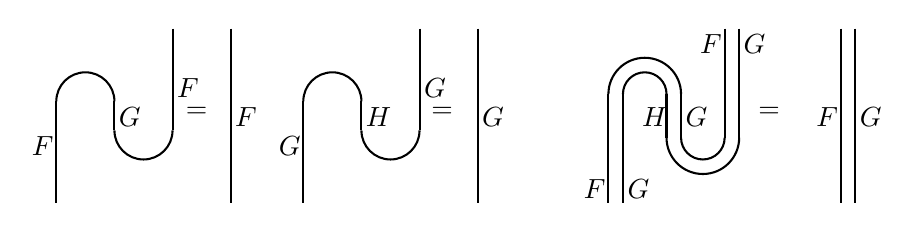
\begin{tikzpicture}[x=0.75pt,y=0.75pt,yscale=-0.7,xscale=0.7]
			%uncomment if require: \path (0,300); %set diagram left start at 0, and has height of 300
			
			%Straight Lines [id:da387661253376389] 
			\draw    (420,205) -- (420,280) ;
			%Shape: Arc [id:dp46713278097768685] 
			\draw  [draw opacity=0] (420,205) .. controls (420,205) and (420,205) .. (420,205) .. controls (420,191.19) and (431.19,180) .. (445,180) .. controls (458.81,180) and (470,191.19) .. (470,205) -- (445,205) -- cycle ; \draw   (420,205) .. controls (420,205) and (420,205) .. (420,205) .. controls (420,191.19) and (431.19,180) .. (445,180) .. controls (458.81,180) and (470,191.19) .. (470,205) ;  
			%Shape: Arc [id:dp15518560403497728] 
			\draw  [draw opacity=0] (500,235) .. controls (500,235) and (500,235) .. (500,235) .. controls (500,243.28) and (493.28,250) .. (485,250) .. controls (476.72,250) and (470,243.28) .. (470,235) -- (485,235) -- cycle ; \draw   (500,235) .. controls (500,235) and (500,235) .. (500,235) .. controls (500,243.28) and (493.28,250) .. (485,250) .. controls (476.72,250) and (470,243.28) .. (470,235) ;  
			%Straight Lines [id:da32241416100744336] 
			\draw    (500,160) -- (500,235) ;
			%Straight Lines [id:da38856781567044685] 
			\draw    (470,205) -- (470,235) ;
			%Straight Lines [id:da03391852666101669] 
			\draw    (580,160) -- (580,280) ;
			%Straight Lines [id:da26245589864663876] 
			\draw    (590,160) -- (590,280) ;
			%Shape: Arc [id:dp9620812953682365] 
			\draw  [draw opacity=0] (430,205) .. controls (430,205) and (430,205) .. (430,205) .. controls (430,196.72) and (436.72,190) .. (445,190) .. controls (453.28,190) and (460,196.72) .. (460,205) -- (445,205) -- cycle ; \draw   (430,205) .. controls (430,205) and (430,205) .. (430,205) .. controls (430,196.72) and (436.72,190) .. (445,190) .. controls (453.28,190) and (460,196.72) .. (460,205) ;  
			%Straight Lines [id:da264678990750177] 
			\draw    (430,205) -- (430,280) ;
			%Straight Lines [id:da4480862128459262] 
			\draw    (460,205) -- (460,235) ;
			%Shape: Arc [id:dp4854117335652133] 
			\draw  [draw opacity=0] (510,235) .. controls (510,235) and (510,235) .. (510,235) .. controls (510,248.81) and (498.81,260) .. (485,260) .. controls (471.19,260) and (460,248.81) .. (460,235) -- (485,235) -- cycle ; \draw   (510,235) .. controls (510,235) and (510,235) .. (510,235) .. controls (510,248.81) and (498.81,260) .. (485,260) .. controls (471.19,260) and (460,248.81) .. (460,235) ;  
			%Straight Lines [id:da5773195456674756] 
			\draw    (510,160) -- (510,235) ;
			%Straight Lines [id:da3677305567714848] 
			\draw    (40,210) -- (40,280) ;
			%Shape: Arc [id:dp44820503486725705] 
			\draw  [draw opacity=0] (40,210) .. controls (40,198.95) and (48.95,190) .. (60,190) .. controls (71.05,190) and (80,198.95) .. (80,210) -- (60,210) -- cycle ; \draw   (40,210) .. controls (40,198.95) and (48.95,190) .. (60,190) .. controls (71.05,190) and (80,198.95) .. (80,210) ;  
			%Shape: Arc [id:dp09802818893547105] 
			\draw  [draw opacity=0] (120,230) .. controls (120,230) and (120,230) .. (120,230) .. controls (120,230) and (120,230) .. (120,230) .. controls (120,241.05) and (111.05,250) .. (100,250) .. controls (88.95,250) and (80,241.05) .. (80,230) -- (100,230) -- cycle ; \draw   (120,230) .. controls (120,230) and (120,230) .. (120,230) .. controls (120,230) and (120,230) .. (120,230) .. controls (120,241.05) and (111.05,250) .. (100,250) .. controls (88.95,250) and (80,241.05) .. (80,230) ;  
			%Straight Lines [id:da7148644759520184] 
			\draw    (120,160) -- (120,230) ;
			%Straight Lines [id:da9313139023506238] 
			\draw    (80,210) -- (80,230) ;
			%Straight Lines [id:da4995075644480662] 
			\draw    (160,160) -- (160,280) ;
			%Straight Lines [id:da8345022518562111] 
			\draw    (210,210) -- (210,280) ;
			%Shape: Arc [id:dp11146339353355916] 
			\draw  [draw opacity=0] (210,210) .. controls (210,198.95) and (218.95,190) .. (230,190) .. controls (241.05,190) and (250,198.95) .. (250,210) -- (230,210) -- cycle ; \draw   (210,210) .. controls (210,198.95) and (218.95,190) .. (230,190) .. controls (241.05,190) and (250,198.95) .. (250,210) ;  
			%Shape: Arc [id:dp4903350717792143] 
			\draw  [draw opacity=0] (290,230) .. controls (290,230) and (290,230) .. (290,230) .. controls (290,230) and (290,230) .. (290,230) .. controls (290,241.05) and (281.05,250) .. (270,250) .. controls (258.95,250) and (250,241.05) .. (250,230) -- (270,230) -- cycle ; \draw   (290,230) .. controls (290,230) and (290,230) .. (290,230) .. controls (290,230) and (290,230) .. (290,230) .. controls (290,241.05) and (281.05,250) .. (270,250) .. controls (258.95,250) and (250,241.05) .. (250,230) ;  
			%Straight Lines [id:da4775058157750227] 
			\draw    (290,160) -- (290,230) ;
			%Straight Lines [id:da6968938959124382] 
			\draw    (250,210) -- (250,230) ;
			%Straight Lines [id:da4684865175307644] 
			\draw    (330,160) -- (330,280) ;
			
			% Text Node
			\draw (401,262) node [anchor=north west][inner sep=0.75pt]   [align=left] {$\displaystyle F$};
			% Text Node
			\draw (471,212) node [anchor=north west][inner sep=0.75pt]   [align=left] {$\displaystyle G$};
			% Text Node
			\draw (481,162) node [anchor=north west][inner sep=0.75pt]   [align=left] {$\displaystyle F$};
			% Text Node
			\draw (521,212) node [anchor=north west][inner sep=0.75pt]   [align=left] {$\displaystyle =$};
			% Text Node
			\draw (561,212) node [anchor=north west][inner sep=0.75pt]   [align=left] {$\displaystyle F$};
			% Text Node
			\draw (591,212) node [anchor=north west][inner sep=0.75pt]   [align=left] {$\displaystyle G$};
			% Text Node
			\draw (431,262) node [anchor=north west][inner sep=0.75pt]   [align=left] {$\displaystyle G$};
			% Text Node
			\draw (441,212) node [anchor=north west][inner sep=0.75pt]   [align=left] {$\displaystyle H$};
			% Text Node
			\draw (511,162) node [anchor=north west][inner sep=0.75pt]   [align=left] {$\displaystyle G$};
			% Text Node
			\draw (21,232) node [anchor=north west][inner sep=0.75pt]   [align=left] {$\displaystyle F$};
			% Text Node
			\draw (81,212) node [anchor=north west][inner sep=0.75pt]   [align=left] {$\displaystyle G$};
			% Text Node
			\draw (121,192) node [anchor=north west][inner sep=0.75pt]   [align=left] {$\displaystyle F$};
			% Text Node
			\draw (127,212) node [anchor=north west][inner sep=0.75pt]   [align=left] {$\displaystyle =$};
			% Text Node
			\draw (161,212) node [anchor=north west][inner sep=0.75pt]   [align=left] {$\displaystyle F$};
			% Text Node
			\draw (191,232) node [anchor=north west][inner sep=0.75pt]   [align=left] {$\displaystyle G$};
			% Text Node
			\draw (251,212) node [anchor=north west][inner sep=0.75pt]   [align=left] {$\displaystyle H$};
			% Text Node
			\draw (291,192) node [anchor=north west][inner sep=0.75pt]   [align=left] {$\displaystyle G$};
			% Text Node
			\draw (296,212) node [anchor=north west][inner sep=0.75pt]   [align=left] {$\displaystyle =$};
			% Text Node
			\draw (331,212) node [anchor=north west][inner sep=0.75pt]   [align=left] {$\displaystyle G$};
			
			
		\end{tikzpicture}
	\end{center}
\end{proof}

\begin{prop}
	[label={adjoint-triple-full-faithful}]
	{}
	对于定义 \ref{adjoint-triple} 中的伴随三元组 $F\dashv G\dashv H$,
	第一个伴随的单位 $\operatorname{id}_{\mathcal D} \to GF$ 为同构当且仅当第二个伴随的余单位 $GH\to \operatorname{id}_{\mathcal D}$ 为同构. 因此, 由命题 \ref{adjoint-full-faithful-unit-iso}, $F$ 全忠实当且仅当 $H$ 全忠实.
\end{prop}
\begin{proof}
	考虑如下交换图,
	% https://q.uiver.app/#q=WzAsNCxbMCwwLCJcXG9wZXJhdG9ybmFtZXtIb219KFgsWSkiXSxbMSwwLCJcXG9wZXJhdG9ybmFtZXtIb219KFgsR0goWSkpIl0sWzAsMSwiXFxvcGVyYXRvcm5hbWV7SG9tfShHRihYKSxZKSJdLFsxLDEsIlxcb3BlcmF0b3JuYW1le0hvbX0oRihYKSxIKFkpKSJdLFsyLDAsIlxcb3BlcmF0b3JuYW1le0hvbX0oXFxldGFfWCxZKSJdLFsxLDAsIlxcb3BlcmF0b3JuYW1le0hvbX0oWCxcXHZhcmVwc2lsb25fWSkiLDJdLFszLDEsIlxcc2ltZXEiLDJdLFszLDIsIlxcc2ltZXEiXV0=
	\[\begin{tikzcd}[ampersand replacement=\&]
		{\operatorname{Hom}(X,Y)} \& {\operatorname{Hom}(X,GH(Y))} \\
		{\operatorname{Hom}(GF(X),Y)} \& {\operatorname{Hom}(F(X),H(Y))}
		\arrow["{\operatorname{Hom}(\eta_X,Y)}", from=2-1, to=1-1]
		\arrow["{\operatorname{Hom}(X,\varepsilon_Y)}"', from=1-2, to=1-1]
		\arrow["\simeq"', from=2-2, to=1-2]
		\arrow["\simeq", from=2-2, to=2-1]
	\end{tikzcd}\]
	伴随给出右边与下边的同构, 故左边为同构当且仅当上边为同构.
	由米田引理即证.
\end{proof}

\subsection{伴随函子的 Frobenius 互反律}

Frobenius 互反律是在代数拓扑, 表示论, 逻辑等等许多场合出现的一种重要现象.

\begin{definition}
	[label={Frobenius-reciprocity}]
	{(Frobenius 互反律)}
	设范畴 $\mathcal C,\mathcal D$ 具有乘积, 考虑一对伴随函子 $\begin{tikzcd}[ampersand replacement=\&]
		{\mathcal C} \& {\mathcal D}
		\arrow[""{name=0, anchor=center, inner sep=0}, "f_!", shift left=2, from=1-1, to=1-2]
		\arrow[""{name=1, anchor=center, inner sep=0}, "f^*", shift left=2, from=1-2, to=1-1]
		\arrow["\dashv"{anchor=center, rotate=-90}, draw=none, from=1, to=0]
	\end{tikzcd}%\adj{f_!}{f^*}{\mathcal C}{\mathcal D}
	$. 若对 $\mathcal C$ 的任意对象 $X$ 与 $\mathcal D$ 的任意对象 $Y$, 典范的\emph{投影映射}
	\[
	\pi\colon f_!(f^*Y\times X) \to Y\times f_!(X)
	\]
	为同构, 则称这对伴随满足 \emph{Frobenius 互反律} (reciprocity).
	这个概念还可推广到更一般的幺半范畴, 其中乘积推广为某种运算 $\otimes$, 要求 $f^*$ 保持 $\otimes$.
\end{definition}

% 可以写的东西:

% 与六函子的关系

% separated geometric morphism

% open geometric morphism, Beck--Chevalley
% SGL p494

\begin{prop}
	[label={base-change-Frobenius}]
	{(基变换)}
	设范畴 $\mathcal C$ 存在拉回, 对于态射 $f\colon X\to Y$, 记 $f_!=\Sigma_f$ 为拉回 $f^*\colon \mathcal C/Y \to \mathcal C/X$ 的左伴随 (命题 \ref{sigma-adjoint}), 那么这对伴随满足 Frobenius 互反律.
\end{prop}
\begin{proof}
	此时 Frobenius 互反律说的是对任意态射 $U\to X$ 与 $V\to Y$, $f^*V\times_X U\simeq U\times_Y U$. 这是因为下图中两个小方块为拉回, 故大长方形为拉回.
	% https://q.uiver.app/#q=WzAsNixbMCwwLCJcXCFcXCFcXCFcXCFmXipWXFx0aW1lc19YIFUiXSxbMCwxLCJVIl0sWzEsMCwiZl4qViJdLFsxLDEsIlgiXSxbMiwxLCJZIl0sWzIsMCwiViJdLFsyLDNdLFszLDRdLFsyLDVdLFs1LDRdLFswLDFdLFsxLDNdLFswLDJdXQ==
	\[\begin{tikzcd}[ampersand replacement=\&]
		{\!\!\!\!f^*V\times_X U} \& {f^*V} \& V \\
		U \& X \& Y
		\arrow[from=1-2, to=2-2]
		\arrow[from=2-2, to=2-3]
		\arrow[from=1-2, to=1-3]
		\arrow[from=1-3, to=2-3]
		\arrow[from=1-1, to=2-1]
		\arrow[from=2-1, to=2-2]
		\arrow[from=1-1, to=1-2]
	\end{tikzcd}\]
\end{proof}

\begin{prop}
	[label={ccc-Frobenius-pullback-preserve-exp}]
	{}
	设范畴 $\mathcal C,\mathcal D$ 存在拉回, 且为积闭范畴 (定义 \ref{exponential-object}). 对于伴随函子 $\begin{tikzcd}[ampersand replacement=\&]
		{\mathcal C} \& {\mathcal D}
		\arrow[""{name=0, anchor=center, inner sep=0}, "f_!"', shift right=2, from=1-1, to=1-2]
		\arrow[""{name=1, anchor=center, inner sep=0}, "f^*"', shift right=2, from=1-2, to=1-1]
		\arrow["\dashv"{anchor=center, rotate=-90}, draw=none, from=0, to=1]
	\end{tikzcd}%\adj{f_!}{f^*}{\mathcal C}{\mathcal D}
	$, 其满足 Frobenius 互反律当且仅当 $f^*$ 保持指数对象.
\end{prop}
\begin{proof}
	Frobenius 互反律说的是下图的外层方块交换, 而 $f^*$ 保持指数对象说的是下图的里层方块交换; 由伴随的唯一性, 两者等价.
	\[\begin{tikzcd}[ampersand replacement=\&,column sep=1.7em]
		{\mathcal D} \&\& {\mathcal D} \\
		\\
		{\mathcal C} \&\& {\mathcal C}
		\arrow[""{name=0, anchor=center, inner sep=0}, "{(-)^W}"', shift right=2, from=1-1, to=1-3]
		\arrow[""{name=1, anchor=center, inner sep=0}, "{(-)\times W}"', shift right=2, from=1-3, to=1-1]
		\arrow[""{name=2, anchor=center, inner sep=0}, "{f_!}"', shift right=2, from=3-3, to=1-3]
		\arrow[""{name=3, anchor=center, inner sep=0}, "{f^*}"', shift right=2, from=1-3, to=3-3]
		\arrow[""{name=4, anchor=center, inner sep=0}, "{f^*}", shift left=2, from=1-1, to=3-1]
		\arrow[""{name=5, anchor=center, inner sep=0}, "{(-)^{f^*W}}", shift left=2, from=3-1, to=3-3]
		\arrow[""{name=6, anchor=center, inner sep=0}, "{f_!}", shift left=2, from=3-1, to=1-1]
		\arrow[""{name=7, anchor=center, inner sep=0}, "{(-)\times f^*W}", shift left=2, from=3-3, to=3-1]
		\arrow["\dashv"{anchor=center, rotate=-90}, draw=none, from=1, to=0]
		\arrow["\dashv"{anchor=center, rotate=-180}, draw=none, from=2, to=3]
		\arrow["\dashv"{anchor=center}, draw=none, from=6, to=4]
		\arrow["\dashv"{anchor=center, rotate=90}, draw=none, from=7, to=5]
	\end{tikzcd}\]
\end{proof}
这个结论的推论包括 ``拉回保持指数对象'' (命题 \ref{pullback-preserve-exponential-objects}) 以及位象开映射的等价定义 (命题 \ref{locale-open-map-preserves-implication}).

%\begin{example}
%	{(表示论中的 Frobenius 互反律)}
%	固定一个域 $k$. 对于群 $G$, 所谓 $G$ 的表示是指 $k$-线性空间 $V$ 配备 $G$-作用 $G\to\operatorname{End}_k(V)$, 也即 $k[G]$-模 ($k[G]$ 为群代数, 见例 \ref{algebraic-theory-morphism-example}). 记 $\operatorname{Rep}_G$ 为 $G$ 的表示的范畴.
%	设 $H\hookrightarrow G$ 为子群,
%	那么
%\end{example}

\section{自反子范畴与局部化}
\label{reflective-subcategory-and-localization}

\begin{definition}
	[label={reflective-subcategory}]
	{(自反子范畴, 自反局部化)}
	若一个全子范畴的嵌入 $i\colon \mathcal D\to \mathcal C$ 有左伴随 $a\colon \mathcal C\to\mathcal D$, 则称 $i$ 为\emph{自反子范畴} (reflective subcategory), $a$ 为\emph{自反局部化} (reflective localization).
	\[\begin{tikzcd}[ampersand replacement=\&]
		{\mathcal D} \& {\mathcal C}
		\arrow[""{name=0, anchor=center, inner sep=0}, "i"', shift right=2, hook, from=1-1, to=1-2]
		\arrow[""{name=1, anchor=center, inner sep=0}, "a"', shift right=2, from=1-2, to=1-1]
		\arrow["\dashv"{anchor=center, rotate=-90}, draw=none, from=1, to=0]
	\end{tikzcd}\]
	对于 $\mathcal C$ 的对象 $c$, $a(c)$ 称作 $c$ 的\emph{反映} (reflection).
	若进一步有 $a$ 保持有限极限, 则称之为 (左) \emph{正合局部化} (left-exact localization).
\end{definition}

注意文献中有些地方以 ``局部化'' 代指我们所谓正合局部化.

由定义, 每个对象 $c$ 到其反映有典范的态射 $c \to a(c)$, 来自上述伴随的单位 $\operatorname{id}_{\mathcal C}\to i\circ a$;
而且 $c$ 到 $\mathcal D$ 的任何对象的态射都唯一地穿过这个态射.
由命题 \ref{adjoint-full-faithful-unit-iso},
一对伴随 $\adj{a}{i}{\mathcal {D}}{\mathcal {C}}$%$a\dashv i\colon \mathcal D\leftrightarrows \mathcal C$
构成自反子范畴当且仅当对 $\mathcal D$ 的所有对象 $d$, 余单位 $\varepsilon_d\colon ai(d)\to d$ 为同构.

\begin{example}
	{}
	将偏序集视为范畴, 那么嵌入 $\mathbb{Z}\hookrightarrow\mathbb{R}$ 为自反子范畴, 反映函子 $a\colon \mathbb{R}\to\mathbb{Z}$ 为\emph{向上取整}. 对于实数 $r$ 与整数 $n$, $r\leq n$ 当且仅当 $a(r)\leq n$.
\end{example}

\begin{example}
	{}
	Abel 群范畴 $\mathsf {Ab}$ 是群范畴 $\mathsf {Grp}$ 的自反子范畴, 群 $G$ 的反映是其 Abel 化 (abelianization) $G/[G,G]$.
	类似地, 对于环 $R$, 交换 $R$-代数的范畴是 $R$-代数范畴的自反子范畴, 代数 $A$ 的反映是 $A$ 商掉由交换子生成的理想.
\end{example}

\begin{example}
	[label={localization-module}]
	{}
	设 $R$ 为环, 子集 $S\subset R$ 包含 $1$ 且对乘法封闭\footnotemark{}. $R$ 关于 $S$ 的局部化 $S^{-1}R$ 是
	在 $R$ 中 ``强行使得 $S$ 的元素都可逆'' 得到的环,
	可构造为 ``分式环'' $$
	\Big\{\frac{x}{s} \Bigm| x\in R, s\in S\Big\}\Big/
	\Big(
	\frac{x}{s}\sim\frac{x'}{s'}\Leftrightarrow\exists
	t\in S, t(xs'-x's)=0
	\Big).$$
	$(S^{-1}R)$-模范畴可视为 $R$-模范畴的全子范畴,
	即
	\[
	(S^{-1}R)\mathsf {Mod} \simeq \{ M\in R\mathsf {Mod} \mid \forall s\in S,
	\text{$s$ 在 $M$ 上的作用可逆} \}.
	\]
	$(S^{-1}R)\mathsf {Mod}$ 作为 $R\mathsf {Mod}$ 的自反子范畴,
	其嵌入与反映恰为张量--同态伴随
	\[\begin{tikzcd}[ampersand replacement=\&]
		{(S^{-1}R)\mathsf {Mod}} \& {R\mathsf {Mod}.}
		\arrow[""{name=0, anchor=center, inner sep=0}, "{\operatorname{Hom}(S^{-1}R,-)}"', shift right=2, from=1-1, to=1-2]
		\arrow[""{name=1, anchor=center, inner sep=0}, "{S^{-1}R\otimes -}"', shift right=2, from=1-2, to=1-1]
		\arrow["\dashv"{anchor=center, rotate=-90}, draw=none, from=1, to=0]
	\end{tikzcd}\]
	容易证明 $S^{-1}R\otimes -$ 保持有限极限; 人们称 $S^{-1}R$ 为平坦 $R$-代数.
	在代数--几何对偶中, 局部化可类比为向量丛限制到子空间上的过程.
\end{example}
\footnotetext{这是一种饱和性条件, 其目的是使用\emph{分式计算} (calculus of fractions). 后面我们将介绍范畴的局部化中的类似方法.}

%\begin{definition}
%	[label={reflective-localization}]
%	{(自反局部化)}
%	对于自反子范畴 (\ref{reflective-subcategory}) $$
%	\begin{tikzcd}[ampersand replacement=\&]
%		{\mathcal D} \& {\mathcal C,}
%		\arrow[""{name=0, anchor=center, inner sep=0}, "i"', shift right=2, hook, from=1-1, to=1-2]
%		\arrow[""{name=1, anchor=center, inner sep=0}, "a"', shift right=2, from=1-2, to=1-1]
%		\arrow["\dashv"{anchor=center, rotate=-90}, draw=none, from=1, to=0]
%	\end{tikzcd}
%	$$
%	若左伴随 $a$ 保持有限极限, 则称之为\emph{自反局部化} (reflective localization), 简称\emph{局部化}.
%\end{definition}

%\begin{example}
%	{}
%	拓扑空间 $X$ 上的层范畴 $\operatorname{Sh}(X)$ 是预层范畴 $\text{Presh}(X)$ 的自反局部化, 预层的反映为其层化 (命题 \ref{sheafification}).
%\end{example}

%\todo{澄清不同的局部化概念}
% nLab : https://ncatlab.org/nlab/show/localization+of+a+category
% 

一个范畴 $\mathcal C$ 的全体自反子范畴在包含关系下构成一个偏序集. 关于这个偏序, 有如下实用结论.

\begin{prop}
	[label={reflective-subcategory-poset}]
	{}
	设 $\mathcal D,\mathcal E$ 是 $\mathcal C$ 的自反子范畴, 如图,
	\[\begin{tikzcd}[ampersand replacement=\&]
		{\mathcal D} \& {\mathcal C}
		\arrow[""{name=0, anchor=center, inner sep=0}, "i_1"', shift right=2, hook, from=1-1, to=1-2]
		\arrow[""{name=1, anchor=center, inner sep=0}, "a_1"', shift right=2, from=1-2, to=1-1]
		\arrow["\dashv"{anchor=center, rotate=-90}, draw=none, from=1, to=0]
	\end{tikzcd}
	\begin{tikzcd}[ampersand replacement=\&]
		{\mathcal E} \& {\mathcal C}
		\arrow[""{name=0, anchor=center, inner sep=0}, "i_2"', shift right=2, hook, from=1-1, to=1-2]
		\arrow[""{name=1, anchor=center, inner sep=0}, "a_2"', shift right=2, from=1-2, to=1-1]
		\arrow["\dashv"{anchor=center, rotate=-90}, draw=none, from=1, to=0]
	\end{tikzcd}\]
	则以下条件等价.
	\begin{enumerate}[(1)]
		\item $i_1$ 穿过 $i_2$;
		\item $a_1$ 穿过 $a_2$;
		\item 存在一对伴随 $\begin{tikzcd}[ampersand replacement=\&]
			{\mathcal D} \& {\mathcal E}
			\arrow[""{name=0, anchor=center, inner sep=0}, "i_3"', shift right=2, hook, from=1-1, to=1-2]
			\arrow[""{name=1, anchor=center, inner sep=0}, "a_3"', shift right=2, from=1-2, to=1-1]
			\arrow["\dashv"{anchor=center, rotate=-90}, draw=none, from=1, to=0]
		\end{tikzcd}$ 使得 $i_1=i_2i_3$, $a_1=a_3a_2$.
	\end{enumerate}
\end{prop}

\begin{proof}
	~
	\begin{itemize}
		\item $(3)\Rightarrow (1)$, $(3)\Rightarrow (2)$ 是明显的.
		\item $(1)\Rightarrow (3)$. 令 $a_3 = a_1i_2$ 即可.
		\item $(2)\Rightarrow (3)$. 令 $i_3 = a_2i_1$ 即可.
	\end{itemize}
\end{proof}

自反子范畴中的极限与余极限可由原来范畴中的极限和余极限得到.

\begin{prop}
	[label={co-complete-reflective-subcategory}]
	{(自反子范畴中的极限与余极限)}
	设 $\mathcal D\hookrightarrow \mathcal C$ 为自反子范畴, 记其反映函子为 $a\colon \mathcal C\to\mathcal D$.
	%为避免歧义, 以上标表示极限和余极限所在的范畴; 例如 $\operatorname{lim}^{\mathcal C}$ 表示 $\mathcal C$ 中的极限.
	对任意图 $X\colon I\to \mathcal D$,
	\begin{itemize}
		\item $\operatorname{lim}^{\mathcal D}_i X_i$ 存在当且仅当  $\operatorname{lim}^{\mathcal C}_i X_i$ 存在, 且此时有 $\operatorname{lim}^{\mathcal D}_i X_i\simeq \operatorname{lim}^{\mathcal C}_i X_i$.
		\item 当 $\operatorname{colim}^{\mathcal C}_i X_i$ 存在时, $\operatorname{colim}^{\mathcal D}_i X_i$ 存在, 且有 $\operatorname{colim}^{\mathcal D}_i X_i\simeq a(\operatorname{colim}^{\mathcal C}_i X_i)$, 注意这里需要取 $a$ 下的像.
	\end{itemize}
\end{prop}

\begin{proof}~
	\begin{itemize}
		\item 假设 $\operatorname{lim}^{\mathcal D}_i X_i$ 存在. 嵌入 $\mathcal D\to \mathcal C$ 作为右伴随保持极限, 故 $\operatorname{lim}^{\mathcal C}_i X_i$ 存在且同构于 $\operatorname{lim}^{\mathcal D}_i X_i$.
		\item 假设 $\operatorname{lim}^{\mathcal C}_i X_i$ 存在. 那么有自然同构
		\[
		\begin{aligned}
		\operatorname{Hom}_{\mathcal C}(-,\operatorname{lim}^{\mathcal C}_i X_i)
		&\simeq
		\operatorname{lim}^{\mathsf {Set}}_i\operatorname{Hom}_{\mathcal C}(-,X_i)
		\\&\simeq
		\operatorname{lim}^{\mathsf {Set}}_i\operatorname{Hom}_{\mathcal C}(a(-),X_i)
		\simeq
		\operatorname{Hom}_{\mathcal C}(a(-),\operatorname{lim}^{\mathcal C}_i X_i),
		\end{aligned}
		\]
		这说明 $\operatorname{lim}^{\mathcal C}_i X_i$ 差一个同构落在 $\mathcal D$ 中, 因而 $\operatorname{lim}^{\mathcal D}_i X_i\simeq \operatorname{lim}^{\mathcal C}_i X_i$.
		\item 假设 $\operatorname{colim}^{\mathcal C}_i X_i$ 存在. 反映 $a\colon \mathcal C\to \mathcal D$ 作为左伴随保持余极限, 故 $\operatorname{lim}^{\mathcal D}_i X_i$ 存在且同构于 $a(\operatorname{lim}^{\mathcal C}_i X_i)$.
	\end{itemize}
\end{proof}

自反局部化是一般的局部化概念的特例. 在某些范畴中, 一些态射本来不可逆, 但我们希望它们可逆;
通过局部化我们可以构造一个新的范畴让这些态射变得可逆, 同时新的范畴尽可能逼近原来的范畴.

\begin{definition}
	[label={localization-by-universally-inverting}]
	{(局部化)}
	设 $\mathcal C$ 为范畴, $W$ 为 $\mathcal C$ 中的一族态射.
	若存在范畴 $\mathcal C[W^{-1}]$ 与函子 $a\colon \mathcal C\to \mathcal C[W^{-1}]$ 满足如下条件, 则称之为 $\mathcal C$ 关于 $W$ 的\emph{局部化}.
	\begin{itemize}
		\item 对任意 $w\in W$, $a(w)$ 为同构;
		\item (\emph{万有性质}) 对任意范畴 $\mathcal E$ 与函子 $b\colon \mathcal C\to\mathcal E$, 若 $b$ 将 $W$ 的元素变为同构,
		则 $b$ 穿过 $a$ 有 ``唯一'' 的分解, ``唯一'' 是指两种分解至多差一个唯一的自然同构. 更具体地说, 存在函子 $f\colon \mathcal C[W^{-1}]\to\mathcal E$ 以及自然同构 $\rho\colon b \overset{\simeq}{\to} fa$, 且对任意两个自然同构 $\rho\colon b \overset{\simeq}{\to} fa, \rho'\colon b \overset{\simeq}{\to} f'a$ 都存在唯一的自然同构 $\kappa\colon f\to f'$, 满足 $\rho' = (\kappa\cdot a)\rho$.
		%严格地说, 记 $\mathsf {Fun}_W(\mathcal C,\mathcal E)$ 为 $\mathsf {Fun}(\mathcal C,\mathcal E)$ 中由将 $W$ 的元素变为同构的函子 $b$ 构成的全子范畴,
		%则函子
		%$$(-\circ a)\colon \mathsf {Fun}(\mathcal C[W^{-1}],\mathcal E) \to \mathsf {Fun}_W(\mathcal C,\mathcal E)$$
		%为范畴等价.
	\end{itemize}
\end{definition}

%\begin{remark}
%	{(局部化的概念)}
%	一般的局部化 $\mathcal C \to \mathcal C[W^{-1}]$ 是指使一族态射 $W$ 变为同构的 ``万有'' 过程; 此处的局部化是其特例 (令 $W$ 为所有被 $a$ 变为同构的态射).
%\end{remark}

注意局部化的万有性质是 $2$-范畴中的始对象 (定义 \ref{terminal-object-2-category}), 故 $\mathcal C[W^{-1}]$ 是在范畴等价 (而非范畴同构) 的意义下唯一确定的.

\begin{prop}
	[label={reflective-subcategories-are-localizations}]
	{(自反子范畴是局部化)}
	对于自反子范畴 (\ref{reflective-subcategory}) $$
	\begin{tikzcd}[ampersand replacement=\&]
		{\mathcal D} \& {\mathcal C,}
		\arrow[""{name=0, anchor=center, inner sep=0}, "i"', shift right=2, hook, from=1-1, to=1-2]
		\arrow[""{name=1, anchor=center, inner sep=0}, "a"', shift right=2, from=1-2, to=1-1]
		\arrow["\dashv"{anchor=center, rotate=-90}, draw=none, from=1, to=0]
	\end{tikzcd}
	$$
	记
	$$
	W = \big\{
	\text{$\mathcal C$中的态射$f$} \mid \text{$a(f)$可逆}
	\big\},
	$$
	则函子 $a\colon \mathcal C\to\mathcal D$ 给出定义 \ref{localization-by-universally-inverting} 中的局部化 $\mathcal C[W^{-1}]$.
\end{prop}

\begin{proof}
	我们要证明对任意范畴 $\mathcal E$ 以及函子 $b\colon \mathcal C\to\mathcal E$, 若 $b$ 将 $W$ 的元素变为同构, 则 $b$ 穿过 $a$ 有唯一的分解. 考虑伴随的单位 $\eta\colon \operatorname{id}_{\mathcal C}\to ia$, 作如下自然变换 $\rho\colon b\to bia$.
	% https://q.uiver.app/#q=WzAsNCxbMCwwLCJcXG1hdGhzZiBDIl0sWzEsMSwiXFxtYXRoc2YgRCJdLFsyLDAsIlxcbWF0aHNmIEMiXSxbMywwLCJcXG1hdGhzZiBFIl0sWzAsMSwiYSIsMl0sWzEsMiwiaSIsMix7InN0eWxlIjp7InRhaWwiOnsibmFtZSI6Imhvb2siLCJzaWRlIjoidG9wIn19fV0sWzAsMiwiXFxvcGVyYXRvcm5hbWV7aWR9X3tcXG1hdGhzZiBDfSJdLFsyLDMsImIiXSxbNiwxLCJcXGV0YSIsMCx7InNob3J0ZW4iOnsic291cmNlIjoyMH19XV0=
	\[\rho = b\cdot\eta = \begin{tikzcd}[ampersand replacement=\&,column sep=1.5em]
		{\mathcal C} \&\& {\mathcal C} \& {\mathcal E} \\
		\& {\mathcal D}
		\arrow["a"', from=1-1, to=2-2]
		\arrow["i"', hook, from=2-2, to=1-3]
		\arrow[""{name=0, anchor=center, inner sep=0}, "{\operatorname{id}_{\mathcal C}}", from=1-1, to=1-3]
		\arrow["b", from=1-3, to=1-4]
		\arrow["\eta", shorten <=3pt,shorten >=3pt, Rightarrow, from=0, to=2-2]
	\end{tikzcd}\]
	对 $\mathcal C$ 的每个对象 $c$, 由于 $\eta_c\colon c\to ia(c)$ 被 $a$ 变为同构\footnote{这是由于 ``幂等性'' $iaia\simeq ia$.}, 按定义它也被 $b$ 变为同构.
	因此 $\rho$ 为自然同构.\footnote{若一个自然变换在每个对象上给出同构, 那么它是自然同构.}
	我们得到一个 $b$ 穿过 $a$ 的分解.
	
	对任意一个 $b$ 穿过 $a$ 的分解 $\rho'\colon b\overset{\simeq}{\to}b'a$, 考虑伴随的余单位 $\varepsilon\colon ai\to\operatorname{id}_{\mathcal D}$ (由命题 \ref{reflective-counit-isomorphism} 它对 $\mathcal D$ 的每个对象都给出同构), 我们得到如下自然变换 $\kappa\colon bi\to b'$.
	% https://q.uiver.app/#q=WzAsNCxbMCwxLCJcXG1hdGhzZiBEIl0sWzEsMCwiXFxtYXRoc2YgQyJdLFszLDAsIlxcbWF0aHNmIEUiXSxbMiwxLCJcXG1hdGhzZiBEIl0sWzAsMSwiaSIsMCx7InN0eWxlIjp7InRhaWwiOnsibmFtZSI6Imhvb2siLCJzaWRlIjoidG9wIn19fV0sWzEsMiwiYiJdLFsxLDMsImEiLDFdLFszLDIsImInIiwyXSxbMCwzLCJcXG9wZXJhdG9ybmFtZXtpZH1fe1xcbWF0aHNmIER9IiwyXSxbMSw4LCJcXHZhcmVwc2lsb24iLDIseyJzaG9ydGVuIjp7InNvdXJjZSI6MjAsInRhcmdldCI6MjB9fV0sWzUsMywiIiwwLHsic2hvcnRlbiI6eyJzb3VyY2UiOjIwLCJ0YXJnZXQiOjIwfX1dXQ==
	\[\kappa = \begin{tikzcd}[ampersand replacement=\&,column sep=1.5em]
		\& {\mathcal C} \&\& {\mathcal E} \\
		{\mathcal D} \&\& {\mathcal D}
		\arrow["i", hook, from=2-1, to=1-2]
		\arrow[""{name=0, anchor=center, inner sep=0}, "b", from=1-2, to=1-4]
		\arrow["a"{description}, from=1-2, to=2-3]
		\arrow["{b'}"', from=2-3, to=1-4]
		\arrow[""{name=1, anchor=center, inner sep=0}, "{\operatorname{id}_{\mathcal D}}"', from=2-1, to=2-3]
		\arrow["\varepsilon"', shorten <=3pt, shorten >=3pt, Rightarrow, from=1-2, to=1]
		\arrow["\rho'",shorten <=3pt, shorten >=3pt, Rightarrow, from=0, to=2-3]
	\end{tikzcd}\]
	那么 $\kappa$ 为自然同构. 进一步, 由伴随的定义有如下等式,
	% https://q.uiver.app/#q=WzAsNSxbMSwxLCJcXG1hdGhzZiBEIl0sWzIsMCwiXFxtYXRoc2YgQyJdLFs0LDAsIlxcbWF0aHNmIEUiXSxbMywxLCJcXG1hdGhzZiBEIl0sWzAsMCwiXFxtYXRoc2YgQyJdLFswLDEsImkiLDEseyJzdHlsZSI6eyJ0YWlsIjp7Im5hbWUiOiJob29rIiwic2lkZSI6InRvcCJ9fX1dLFsxLDIsImIiXSxbMSwzLCJhIiwxXSxbMywyLCJiJyIsMl0sWzAsMywiXFxvcGVyYXRvcm5hbWV7aWR9X3tcXG1hdGhzZiBEfSIsMl0sWzQsMSwiXFxvcGVyYXRvcm5hbWV7aWR9X3tcXG1hdGhzZiBDfSJdLFs0LDAsImEiLDJdLFsxLDksIlxcdmFyZXBzaWxvbiIsMix7InNob3J0ZW4iOnsic291cmNlIjoyMCwidGFyZ2V0IjoyMH19XSxbNiwzLCJcXHJobyciLDAseyJzaG9ydGVuIjp7InNvdXJjZSI6MjAsInRhcmdldCI6MjB9fV0sWzEwLDAsIlxcZXRhIiwyLHsic2hvcnRlbiI6eyJzb3VyY2UiOjIwLCJ0YXJnZXQiOjIwfX1dXQ==
	\[\begin{tikzcd}[ampersand replacement=\&,column sep=1.5em]
		{\mathcal C} \&\& {\mathcal C} \&\& {\mathcal E} \\
		\& {\mathcal D} \&\& {\mathcal D}
		\arrow["i"{description}, hook, from=2-2, to=1-3]
		\arrow[""{name=0, anchor=center, inner sep=0}, "b", from=1-3, to=1-5]
		\arrow["a"{description}, from=1-3, to=2-4]
		\arrow["{b'}"', from=2-4, to=1-5]
		\arrow[""{name=1, anchor=center, inner sep=0}, "{\operatorname{id}_{\mathcal D}}"', from=2-2, to=2-4]
		\arrow[""{name=2, anchor=center, inner sep=0}, "{\operatorname{id}_{\mathcal C}}", from=1-1, to=1-3]
		\arrow["a"', from=1-1, to=2-2]
		\arrow["\varepsilon"', shorten <=3pt, shorten >=3pt, Rightarrow, from=1-3, to=1]
		\arrow["{\rho'}", shorten <=3pt, shorten >=3pt, Rightarrow, from=0, to=2-4]
		\arrow["\eta"', shorten <=3pt, shorten >=3pt, Rightarrow, from=2, to=2-2]
	\end{tikzcd}
	=
	\begin{tikzcd}[ampersand replacement=\&,column sep=1.5em]
		{\mathcal C} \&\& {\mathcal E} \\
		\& {\mathcal D}
		\arrow[""{name=0, anchor=center, inner sep=0}, "b", from=1-1, to=1-3]
		\arrow["a"', from=1-1, to=2-2]
		\arrow["{b'}"', from=2-2, to=1-3]
		\arrow["{\rho'}", shorten <=3pt, shorten >=3pt, Rightarrow, from=0, to=2-2]
	\end{tikzcd}\]
	即 $\rho'=(\kappa\cdot a)\rho.$ 这样的 $\kappa$ 是唯一的, 因为 $\rho',\rho$ 均为自然同构, 而 $a$ 是本质满函子.
\end{proof}

\subsection{局部对象}

在自反局部化 (\ref{reflective-subcategories-are-localizations}) 中, 子范畴 $\mathcal D$ 有一种实用的描述:
它是\emph{局部对象}的子范畴.

\begin{definition}
	[label={local-objects}]
	{(局部对象)}
	设 $S$ 是范畴 $\mathcal C$ 中的一族态射, $X$ 为 $\mathcal C$ 的对象. 若对任意 $(f\colon A\to B)\in S$,
	\[
	\operatorname{Hom}(f,X)\colon \operatorname{Hom}(B,X) \to \operatorname{Hom}(A,X)
	\]
	均为双射 (\cite{LPAC} 将这个条件称作 $X$ \emph{垂直}于 $f$), 则称 $X$ 为 $S$-\emph{局部对象} (local object).
	记 $S$-局部对象的全子范畴为 $\mathcal C_S \hookrightarrow \mathcal C$.
\end{definition}

直观上, ``在 $S$-局部对象 $X$ 看来'', $S$ 中的态射 $f\colon A\to B$ 就像是一个同构.


%局部化还可对单个对象谈论.
\begin{definition}
	{($S$-等价)}
	设 $S$ 是范畴 $\mathcal C$ 中的一族态射, $f\colon A\to B$ 为 $\mathcal C$ 中的态射.
	若对任意 $S$-局部对象 $X$,
	\[
	\operatorname{Hom}(f,X)\colon \operatorname{Hom}(B,X) \to \operatorname{Hom}(A,X)
	\]
	均为双射, 则称 $f$ 为 \emph{$S$-等价}.
\end{definition}
\begin{definition}
	{(局部化态射)}
	设 $S$ 是范畴 $\mathcal C$ 中的一族态射. 对于态射 $f\colon X\to X'$, 若 $X'$ 为 $S$-局部对象且 $f$ 为 $S$-等价,
	则称之为 \emph{$S$-局部化态射}.
\end{definition}
%\todo{上述定义放在哪里?}


\begin{example}
	[label={frame-cBa-local-object}]
	{(完备 Boole 代数作为\fm{}范畴的局部对象)}
	考虑一个元素 $a$ 生成的自由\fm{} $\{\bot,a,\top\}$ (定义 \ref{frame-definition}) 与自由 Boole 代数 $\{\bot,a,\neg a,\top\}$. \fm{}范畴 $\mathsf {Frm}$ 中关于态射
	\[
	\{\bot,a,\top\} \hookrightarrow \{\bot, a, \neg a, \top\} 
	\]
	的局部对象为\emph{完备 Boole 代数}.
	\fm{} $\mathcal O(X)$ 的局部化态射是 ``双重否定子位象'' $X_{\neg\neg}\hookrightarrow X$ (例 \ref{double-negation-sublocale}).
\end{example}
\begin{example}
	{(Abel 群作为群范畴的局部对象)}
	考虑 $2$ 个元素生成的自由群 $F_2$ 以及自由 Abel 群 $\mathbb{Z}^2$.
	群范畴 $\mathsf {Grp}$ 中关于态射 $F_2\to \mathbb{Z}^2$ 的局部对象即为 Abel 群.
	群 $G$ 的局部化态射即商映射 $G \to G/[G,G]$.
\end{example}

\begin{prop}
	[label={local-objects-closed-limits}]
	{(局部对象关于极限封闭)}
	设 $S$ 是范畴 $\mathcal C$ 中的一族态射, $X\colon I\to \mathcal C_S\hookrightarrow\mathcal C$ 为 $S$-局部对象的图.
	假设 $X$ 的极限 $\operatorname{lim}_i X_i$ 存在, 那么 $\operatorname{lim}_i X_i$ 是 $S$-局部对象.
\end{prop}
\begin{proof}
	对任意 $(f\colon A\to B)\in S$ 以及 $g\colon A\to \operatorname{lim}_i X_i$,
	由于 $X_i$ 为 $S$-局部对象, 锥 $(\pi_i\circ g\colon A\to X_i)_{i\in I}$ 确定了唯一的锥 $(h_i\colon B \to X_i)_{i\in I}$ 使得下图交换.
	% https://q.uiver.app/#q=WzAsNCxbMCwwLCJBIl0sWzAsMSwiQiJdLFsxLDAsIlxcb3BlcmF0b3JuYW1le2xpbX1faSBYX2kiXSxbMSwxLCJYX2kiXSxbMCwxLCJmIiwyXSxbMiwzLCJcXHBpX2kiXSxbMCwyLCJnIl0sWzEsMywiaF9pIiwyXV0=
	\[\begin{tikzcd}[ampersand replacement=\&]
		A \& {\operatorname{lim}_i X_i} \\
		B \& {X_i}
		\arrow["f"', from=1-1, to=2-1]
		\arrow["{\pi_i}", from=1-2, to=2-2]
		\arrow["g", from=1-1, to=1-2]
		\arrow["{h_i}"', from=2-1, to=2-2]
	\end{tikzcd}\]
\end{proof}

上述性质的应用之一是预层范畴中的层关于极限封闭 (命题 \ref{sheaf-limit}).

\begin{prop}
	{(自反子范畴可视为局部对象的子范畴)}
	沿用命题 \ref{reflective-subcategories-are-localizations} 的记号,
	子范畴 $i\colon \mathcal D\to \mathcal C$ 等价于 $W$-局部对象的全子范畴 $\mathcal C_W \hookrightarrow \mathcal C$.
\end{prop}
\begin{proof}
	对于 $\mathcal D$ 的对象 $X$,
	由于自然同构
	\[
	\operatorname{Hom}_{\mathcal C}(-,i(X)) \simeq \operatorname{Hom}_{\mathcal D}(a(-),X),
	\]
	知 $\operatorname{Hom}_{\mathcal C}(-,i(X))$ 将 $W$ 的元素对应到集合的双射, 即 $i(X)$ 是 $W$-局部对象.
	
	另一方面, 设 $\mathcal C$ 的对象 $Y$ 是 $W$-局部对象, 我们证明 $\eta_Y\colon Y\to ia(Y)$ 为同构.
	首先, $\eta_Y$ 是 $W$ 的元素, 由 $Y$ 是 $W$-局部对象得同构
	\[
	\operatorname{Hom}_{\mathcal C}(\eta_Y,Y)\colon \operatorname{Hom}_{\mathcal C}(ia(Y),Y) \overset{\simeq}{\to} \operatorname{Hom}_{\mathcal C}(Y,Y).
	\]
	考虑右边的元素 $\operatorname{id}_Y$ 在左边的原像, 知 $\eta_Y$ 有左逆 $\eta_Y^{-1}\colon ia(Y)\to Y$.
	但 $ia(Y)$ 也是 $W$-局部对象, 同理可得 $\eta_Y^{-1}$ 有左逆.
	左逆的左逆一定是自身. 这证明了 $\eta_Y\colon Y\to ia(Y)$ 为同构.
\end{proof}

%下面是上述命题某种意义上的逆.
%
%\begin{prop}
%	{}
%	设 $S$ 是可表现范畴 $\mathcal C$ (定义 \ref{presentable-categories}) 中的一族态射,
%	则 $S$-局部对象的子范畴 $\mathcal C_S\hookrightarrow \mathcal C$ 是自反子范畴.
%\end{prop}
%
%\begin{proof}
%\todo{locally presentable category}
%任取 $\mathcal C$ 的对象 $c$. 定义范畴 $S_c$:
%其对象为 $\mathcal C$ 中的 \emph{$S$-等价} $c\to d$,
%态射为如下交换图.
%% https://q.uiver.app/#q=WzAsMyxbMSwwLCJjIl0sWzAsMSwiZSJdLFsyLDEsImQiXSxbMCwxXSxbMSwyXSxbMCwyXV0=
%\[\begin{tikzcd}[ampersand replacement=\&,column sep=tiny]
%	\& c \\
%	e \&\& d
%	\arrow[from=1-2, to=2-1]
%	\arrow[from=2-1, to=2-3]
%	\arrow[from=1-2, to=2-3]
%\end{tikzcd}\]
%我们断言 $c$ 局部化态射是 $S_c$ 的终对象.
%\todo{$S_c$ 可表现}
%可表现范畴是完备范畴 (命题 \ref{presentable-complete}), 故 $S_c$ 有终对象.
%
%对于 $S_c$ 的终对象 $c\to d$, 我们说明 $d$ 为 $S$-局部对象.
%
%\end{proof}

%\todo{LPAC 1.36, 1.37, 1.38, 1.39}

上面说明自反子范畴是局部对象的子范畴; 另一方面, 我们希望局部对象的子范畴是自反子范畴, 从而通过自反子范畴的 ``反映'' $c\to a(c)$, 每个对象 $c$ 都被一个尽可能接近的 $S$-局部对象替代.
这不总是可行的 (例 \ref{frame-cBa-local-object} 的完备 Boole 代数范畴不是自反子范畴), 但对于可表现范畴有一些部分的结论.

\begin{prop}
	[label={local-object-reflective-subcategory}]
	{}
	设 $S$ 是可表现范畴 $\mathcal C$ 中的一族态射构成的\emph{小}集合. 那么 $\mathcal C_S\hookrightarrow \mathcal C$ 为自反子范畴.
\end{prop}

见 \cite{LPAC} 命题 1.36.

\begin{remark}
	[label={strongly-saturated-class-of-morphisms}]
	{(强饱和态射族)}
	对于余完备范畴 $\mathcal C$ 中的一族态射 $S$,
	称其为\emph{强饱和态射族} (strongly saturated class of morphisms) 是指
	$S$ 关于沿 $\mathcal C$ 中任何态射的推出封闭, 关于箭头范畴 $\mathsf {Fun}(\bullet{\to}\bullet,\mathcal C)$ 中的余极限封闭, 且满足三选二性质: 若三个态射 $f,g,h$ 满足 $f=gh$, 只要其中两个属于 $S$, 则三个都属于 $S$.
	
	任何一族态射 $S$ 都生成一个最小的强饱和态射族 $\overline{S}$.
	可以证明, 在命题 \ref{local-object-reflective-subcategory} 中, 对于 $S$-局部对象的子范畴 $\mathcal C_S \hookrightarrow\mathcal C$ 的左伴随 $a\colon \mathcal C\to\mathcal C_S$,
	被 $a$ 变为同构的态射的族恰为 $\overline{S}$.
	\cite{HTT} 5.5.4.15 证明了这一命题的 $\infty$-范畴版本, 当然它可以逐字翻译为普通范畴的版本.
\end{remark}

\begin{prop}
	{(正合局部化的判定)}
	设 $\mathcal C$ 具有有限极限, 沿用命题 \ref{reflective-subcategories-are-localizations} 的记号,
	$a$ 是正合局部化当且仅当 $W$ 关于基变换稳定, 即 $W$ 的元素的拉回仍是 $W$ 的元素.
\end{prop}
\begin{proof}
	该证明取自 \nlab.\footnote{\url{https://ncatlab.org/nlab/show/reflective+sub-(infinity,1)-category}} 命题的一半是显然的: 假设 $a$ 是正合局部化, 那么 $a$ 保持拉回, 而同构的拉回为同构, 故 $W$ 的元素的拉回仍是 $W$ 的元素.
	
	另一方面, 假设 $W$ 关于基变换稳定.
	首先, 因为 $\mathcal C$ 的终对象显然是 $W$-局部对象, 所以 $a$ 保持终对象.
	下面证明 $a$ 保持拉回.
	注意 $W$ 满足 ``三选二性质'': 若三个态射 $f,g,h$ 满足 $f=gh$, 只要其中两个属于 $W$, 则三个都属于 $W$.
	考虑任意两个态射 $X\to Y \leftarrow Z$.
	以下论证中涉及的态射 $X\to a(X)$ 默认为伴随的单位 $\eta_X$. 注意 $\eta_X \in W$.
	
	容易说明 $a(X)\times_{a(Y)} a(Z)$ 是 $W$-局部对象.
	因此, 要证明 $a$ 保持拉回, 只需证明 $(X\times_Y Z \to a(x)\times_{a(Y)} a(Z)) \in W$.
	将其分解为
	\[
	X\times_Y Z \to X\times_{a(Y)}Z \to a(x)\times_{a(Y)}Z \to a(x)\times_{a(Y)} a(Z).
	\]
	只需证明这三个态射均属于 $W$.
	\begin{itemize}
		\item 对于第一个态射 $X\times_Y Z \to X\times_{a(Y)} Z$,
		它是 $\Delta\colon Y\to Y\times_{a(Y)}Y$ 的拉回 (左下图),
		又
		$\pi_1\Delta = \operatorname{id}_Y$,
		$\pi_1$ 是右下图的拉回.
		% https://q.uiver.app/#q=WzAsNCxbMCwxLCJYXFx0aW1lc197YShZKX1aIl0sWzEsMSwiWVxcdGltZXNfe2EoWSl9WSJdLFswLDAsIlhcXHRpbWVzX3tZfVoiXSxbMSwwLCJZIl0sWzIsMF0sWzAsMV0sWzIsM10sWzMsMSwiXFxEZWx0YSJdXQ==
		\[\begin{tikzcd}[ampersand replacement=\&]
			{X\times_{Y}Z} \& Y \\
			{X\times_{a(Y)}Z} \& {Y\times_{a(Y)}Y}
			\arrow[from=1-1, to=2-1]
			\arrow[from=2-1, to=2-2]
			\arrow[from=1-1, to=1-2]
			\arrow["\Delta", from=1-2, to=2-2]
		\end{tikzcd}
		\begin{tikzcd}[ampersand replacement=\&,row sep=small,column sep=tiny]
			{Y\times_{a(Y)}Y} \& Y \\
			Y \& {a(Y)}
			\arrow["{\pi_1}"', from=1-1, to=2-1]
			\arrow["\eta_Y"',from=2-1, to=2-2]
			\arrow["{\pi_2}", from=1-1, to=1-2]
			\arrow["\eta_Y",from=1-2, to=2-2]
		\end{tikzcd}\]
		\item 第二个和第三个态射的原理相同; 第二个态射是如下的拉回.
		% https://q.uiver.app/#q=WzAsNixbMCwxLCJhKFgpXFx0aW1lc197YShZKX1aIl0sWzEsMSwiYShYKVxcdGltZXMgWiJdLFswLDAsIlhcXHRpbWVzX3thKFkpfVoiXSxbMSwwLCJYXFx0aW1lcyBaIl0sWzIsMCwiWCJdLFsyLDEsImEoWCkiXSxbMiwwXSxbMCwxLCIiLDAseyJzdHlsZSI6eyJ0YWlsIjp7Im5hbWUiOiJob29rIiwic2lkZSI6InRvcCJ9fX1dLFsyLDMsIiIsMCx7InN0eWxlIjp7InRhaWwiOnsibmFtZSI6Imhvb2siLCJzaWRlIjoidG9wIn19fV0sWzMsMSwiXFxldGFfWFxcdGltZXMgXFxvcGVyYXRvcm5hbWV7aWR9X1oiXSxbNCw1LCJcXGV0YV9YIl0sWzMsNF0sWzEsNV1d
		\[\begin{tikzcd}[ampersand replacement=\&]
			{X\times_{a(Y)}Z} \& {X\times Z} \& X \\
			{a(X)\times_{a(Y)}Z} \& {a(X)\times Z} \& {a(X)}
			\arrow[from=1-1, to=2-1]
			\arrow[hook, from=2-1, to=2-2]
			\arrow[hook, from=1-1, to=1-2]
			\arrow["{\eta_X\times \operatorname{id}_Z}", from=1-2, to=2-2]
			\arrow["{\eta_X}", from=1-3, to=2-3]
			\arrow[from=1-2, to=1-3]
			\arrow[from=2-2, to=2-3]
		\end{tikzcd}\]
	\end{itemize}
\end{proof}

\begin{prop}
	[label={exponential-ideal-cartesian-closed-reflective-subcategory}]
	{(指数理想的判定)}
	设 $\mathcal C$ 为积闭范畴, $\mathcal D$ 为自反子范畴, 反映函子为 $a$.
	称 $\mathcal D$ 为\emph{指数理想} (exponential ideal) 是指对任意 $\mathcal C$ 的对象 $X$ 与 $\mathcal D$ 的对象 $Y$, 都有 $Y^X$ 为 $\mathcal D$ 的对象 (至多相差一个同构).
	那么 $\mathcal D$ 为指数理想当且仅当 $a$ 保持有限积.
\end{prop}
\begin{proof}
	由于 $a$ 保持有限积且 $aa=a$, 有自然同构
	$a(Z\times X)\simeq a(Z)\times a(X)\simeq a(a(Z)\times X)$,
	\begin{align*}
		\operatorname{Hom}_{ {\mathcal C}} (Z,Y^X)&\simeq
		\operatorname{Hom}_{ {\mathcal C}} (Z\times X,Y)\\
		&\simeq \operatorname{Hom}_{ {\mathcal C}} (a(Z\times X),Y)\\
		&\simeq \operatorname{Hom}_{ {\mathcal C}} (a(a(Z)\times X),Y)\\
		&\simeq \operatorname{Hom}_{ {\mathcal C}} (a(Z)\times X,Y)\simeq \operatorname{Hom}_{ {\mathcal C}} (a(Z),Y^X),
	\end{align*}
	故任何态射 $Z\to Y^X$ 唯一地穿过 $Z\to a(Z)$, 这说明 $Y^X$ 是 $\mathcal D$ 的对象.
	
	另一方面, 假设对任意 $\mathcal C$ 的对象 $X$ 与 $\mathcal D$ 的对象 $Y$, 都有 $Y^X$ 为 $\mathcal D$ 的对象.
	那么有自然同构
	\begin{align*}
		\operatorname{Hom}_{ {\mathcal C}}(Z\times X, Y)&\simeq
		\operatorname{Hom}_{ {\mathcal C}}(Z, Y^X)\\
		&\simeq \operatorname{Hom}_{ {\mathcal C}}(a(Z), Y^X)\\
		&\simeq \operatorname{Hom}_{ {\mathcal C}}(a(Z)\times X, Y)\simeq \operatorname{Hom}_{ {\mathcal C}}(a(Z)\times a(X), Y).
	\end{align*}
	故任何态射 $Z\times X\to Y$ 唯一地穿过 $Z\times X \to a(Z)\times a(X)$,
	这说明 $a(Z)\times a(X)\simeq a(Z\times X)$.
\end{proof}

% Elephant 4.3.1

\subsection{分式计算}


局部化 $\mathcal C[W^{-1}]$ 有一种明显的构造: 其对象与 $\mathcal C$ 相同, 而态射为折线形的图表
% https://q.uiver.app/#q=WzAsOSxbMywwLCJcXGJ1bGxldCJdLFsyLDEsIlxcYnVsbGV0Il0sWzQsMSwiXFxidWxsZXQiXSxbNiwxLCJcXGJ1bGxldCJdLFs3LDAsIlxcYnVsbGV0Il0sWzgsMSwiXFxidWxsZXQiXSxbMSwwLCJcXGJ1bGxldCJdLFswLDEsIlxcYnVsbGV0Il0sWzUsMCwiXFxjZG90cyJdLFswLDEsIndfMiIsMl0sWzAsMiwiZl8yIl0sWzQsMywid19yIiwyXSxbNCw1LCJmX3IiXSxbNiw3LCJ3XzEiLDJdLFs2LDEsImZfMSJdLFs4LDIsIiIsMix7InNob3J0ZW4iOnsic291cmNlIjo0MH19XSxbOCwzLCIiLDAseyJzaG9ydGVuIjp7InNvdXJjZSI6NDB9fV1d
\[\begin{tikzcd}[ampersand replacement=\&,row sep=tiny,column sep=small]
	\& \bullet \&\& \bullet \&\& \cdots \&\& \bullet \\
	\bullet \&\& \bullet \&\& \bullet \&\& \bullet \&\& \bullet
	\arrow["{w_2}"', from=1-4, to=2-3]
	\arrow["{f_2}", from=1-4, to=2-5]
	\arrow["{w_r}"', from=1-8, to=2-7]
	\arrow["{f_r}", from=1-8, to=2-9]
	\arrow["{w_1}"', from=1-2, to=2-1]
	\arrow["{f_1}", from=1-2, to=2-3]
	\arrow[shorten <=8pt, from=1-6, to=2-5]
	\arrow[shorten <=8pt, from=1-6, to=2-7]
\end{tikzcd}\,(w_i\in W).\]
实践中未必需要如此复杂的态射. 正如环的局部化 $S^{-1}R$ 的元素可写成分式 $x/s\,(s\in S)$, 我们也希望范畴的局部化 $\mathcal C[W^{-1}]$ 中态射可写成 $fw^{-1}$ ($w\in W$), 如下图.
将态射写成这种形式的方法称作\emph{右分式计算}\footnote{这里 $fw^{-1}$ 是一个纯粹形式的记号. 称之为 ``右分式'' 的原因是 $w^{-1}$ 在右边, 但这种称呼在文献中并不统一.}. 这对态射族 $W$ 有一定的要求.
% https://q.uiver.app/#q=WzAsMyxbMSwwLCJcXGJ1bGxldCJdLFswLDEsIlxcYnVsbGV0Il0sWzIsMSwiXFxidWxsZXQiXSxbMCwxLCJ3IiwyXSxbMCwyLCJmIl0sWzEsMiwiZndeey0xfSIsMix7InN0eWxlIjp7ImJvZHkiOnsibmFtZSI6ImRhc2hlZCJ9fX1dXQ==
\[\begin{tikzcd}[ampersand replacement=\&,sep=small]
	\& \bullet \\
	\bullet \&\& \bullet
	\arrow["w"', from=1-2, to=2-1]
	\arrow["f", from=1-2, to=2-3]
	\arrow["{fw^{-1}}"', dashed, from=2-1, to=2-3]
\end{tikzcd}\]

\begin{definition}
	[label={calculus-of-fractions}]
	{(分式计算)}
	若范畴 $\mathcal C$ 中的一族态射 $W$ 满足如下条件, 则称 $(\mathcal C,W)$ 具有\emph{右分式计算} (calculus of right fractions):
	\begin{enumerate}
		\item[(0)] $W$ 包含所有恒等态射, 且关于态射复合封闭;
		\item[(1)] 如图, 给定 $w\in W$ 与 $f$, 总存在 $w'\in W$ 与 $f'$ 使下图交换;
		\[\begin{tikzcd}[ampersand replacement=\&,sep=small]
			\bullet \& \bullet \\
			\bullet \& \bullet
			\arrow["{w'}"', dashed, from=1-1, to=2-1]
			\arrow["f"', from=2-1, to=2-2]
			\arrow["{f'}", dashed, from=1-1, to=1-2]
			\arrow["w", from=1-2, to=2-2]
		\end{tikzcd}\]
		\item[(2)] 
		如图, 若 $w\in W$ 余等化 $f,g$, 总存在 $w'\in W$ 等化 $f,g$.
		\[\begin{tikzcd}[ampersand replacement=\&,sep=small]
			\bullet \& \bullet \& \bullet \& \bullet
			\arrow["{w'}", dashed, from=1-1, to=1-2]
			\arrow["f", shift left, from=1-2, to=1-3]
			\arrow["w", from=1-3, to=1-4]
			\arrow["g"', shift right, from=1-2, to=1-3]
		\end{tikzcd}\]
	\end{enumerate}
\end{definition}

设计条件 $(1)(2)$ 是为了如下的命题.

\begin{propdef}
	{(分式计算的构造)}
	设 $(\mathcal C,W)$ 具有右分式计算. 如下构造定义了范畴 $\mathcal C[W^{-1}]$.
	\begin{itemize}
		\item 其对象为 $\mathcal C$ 的对象;
		\item 态射 $X\to Y$ 为 $\mathcal C$ 中图表 $fw^{-1}:= \begin{tikzcd}[ampersand replacement=\&,sep=tiny]
			\& \bullet \\
			X \&\& Y
			\arrow["w"', from=1-2, to=2-1]
			\arrow["f", from=1-2, to=2-3]
		\end{tikzcd}$ 的等价类,
		其中 $w\in W$;
		\item 两个态射 $fw^{-1}$, $f' (w')^{-1}$ 等价是指存在 $s,t$ 使得下图交换, 且 $ws = w't \in W$;
		% https://q.uiver.app/#q=WzAsNSxbMCwyLCJYIl0sWzQsMiwiWSJdLFsxLDEsIlxcYnVsbGV0Il0sWzMsMSwiXFxidWxsZXQiXSxbMiwwLCJcXGJ1bGxldCJdLFsyLDAsInciLDJdLFsyLDEsImYiLDIseyJsYWJlbF9wb3NpdGlvbiI6NzB9XSxbMywwLCJ3JyIsMCx7ImxhYmVsX3Bvc2l0aW9uIjo3MH1dLFszLDEsImYnIl0sWzQsMiwicyIsMl0sWzQsMywidCJdXQ==
		\[\begin{tikzcd}[ampersand replacement=\&,sep=tiny]
			\&\& \bullet \\
			\& \bullet \&\& \bullet \\
			X \&\&\&\& Y
			\arrow["w"', from=2-2, to=3-1]
			\arrow["f"'{pos=0.7}, from=2-2, to=3-5]
			\arrow["{w'}"{pos=0.7}, from=2-4, to=3-1]
			\arrow["{f'}", from=2-4, to=3-5]
			\arrow["s"', from=1-3, to=2-2]
			\arrow["t", from=1-3, to=2-4]
		\end{tikzcd}\]
		(我们也可将这种等价做成一个 $2$-态射, 从而形成一个 $2$-范畴.)
		\item 态射的复合: 给定图中的 $f,w,g,v$ ($w,v\in W$), 由定义 \ref{calculus-of-fractions} $(1)$, 存在 $f',v'$ ($v'\in W$) 使下图交换.
		% https://q.uiver.app/#q=WzAsNixbMCwyLCJYIl0sWzIsMiwiWSJdLFsxLDEsIlxcYnVsbGV0Il0sWzMsMSwiXFxidWxsZXQiXSxbMiwwLCJcXGJ1bGxldCJdLFs0LDIsIloiXSxbMiwwLCJ3IiwyXSxbMiwxLCJmIiwyXSxbMywxLCJ2Il0sWzQsMiwidiciLDJdLFs0LDMsImYnIl0sWzMsNSwiZyJdXQ==
		\[\begin{tikzcd}[ampersand replacement=\&,sep=tiny]
			\&\& \bullet \\
			\& \bullet \&\& \bullet \\
			X \&\& Y \&\& Z
			\arrow["w"', from=2-2, to=3-1]
			\arrow["f"', from=2-2, to=3-3]
			\arrow["v", from=2-4, to=3-3]
			\arrow["{v'}"', from=1-3, to=2-2]
			\arrow["{f'}", from=1-3, to=2-4]
			\arrow["g", from=2-4, to=3-5]
		\end{tikzcd}\]
		定义 $(gv^{-1})\circ (fw^{-1})$ 为 $(gf') (wv')^{-1}$.
	\end{itemize}
\end{propdef}

\begin{proof}
	我们需要证明上面的等价关系以及态射复合的良定性. 首先证明一个引理:
	在定义 \ref{calculus-of-fractions} $(1)$ 中, 态射 $f'(w')^{-1}$ 的等价类是唯一确定的.
	考虑下图, 给定 $f,w,f',w',f'',w''$ ($w,w',w''\in W$), 取 $g,v$ ($v\in W$) 使 $w'' g = w v$.
	% https://q.uiver.app/#q=WzAsNyxbMSwxLCJcXGJ1bGxldCJdLFsxLDIsIlxcYnVsbGV0Il0sWzMsMiwiXFxidWxsZXQiXSxbMywwLCJcXGJ1bGxldCJdLFsyLDAsIlxcYnVsbGV0Il0sWzEsMCwiXFxidWxsZXQiXSxbMCwwLCJcXGJ1bGxldCJdLFswLDEsIncnIiwyXSxbMSwyLCJmIiwyXSxbMCwzLCJmJyIsMix7ImxhYmVsX3Bvc2l0aW9uIjo3MH1dLFszLDIsInciXSxbNCwxLCJ3JyciLDAseyJsYWJlbF9wb3NpdGlvbiI6ODB9XSxbNCwzLCJmJyciXSxbNSwwLCJ2IiwyXSxbNSw0LCJnIl0sWzYsNSwiXFx3aWRldGlsZGUge3d9Il1d
	\[\begin{tikzcd}[ampersand replacement=\&]
		\bullet \& \bullet \& \bullet \& \bullet \\
		\& \bullet \\
		\& \bullet \&\& \bullet
		\arrow["{w'}"', from=2-2, to=3-2]
		\arrow["f"', from=3-2, to=3-4]
		\arrow["{f'}"'{pos=0.7}, from=2-2, to=1-4]
		\arrow["w", from=1-4, to=3-4]
		\arrow["{w''}"{pos=0.8}, from=1-3, to=3-2]
		\arrow["{f''}", from=1-3, to=1-4]
		\arrow["v"', from=1-2, to=2-2]
		\arrow["g", from=1-2, to=1-3]
		\arrow["{\widetilde {w}}", from=1-1, to=1-2]
	\end{tikzcd}\]
	此时不一定有 $f''g = f'v$, 但有 $wf''g = wf'v$; 由定义 \ref{calculus-of-fractions} $(2)$,
	存在 $\widetilde {w}\in W$ 使得 $f''g\widetilde w = f'v\widetilde w$.
	这证明了 $f'(w')^{-1}$ 与 $f''(w'')^{-1}$ 等价.
	
	下面说明等价关系的传递性. 考虑下图, 给定 $f_1,w_1,f_2,w_2,f_3,w_3$ ($w_1,w_2,w_3\in W$), 以及 $p,q,s,t$ 构成 $f_1w_1^{-1},f_2w_2^{-1},f_3w_3^{-1}$ 之间的两个等价, 我们要证明 $f_1w_1^{-1}$ 与 $f_3w_3^{-1}$ 等价.
	\[\begin{tikzcd}[ampersand replacement=\&]
		\bullet \& \bullet \& \bullet \\
		\bullet \& \bullet \& \bullet \\
		\bullet \& \bullet
		\arrow["{w_1}"', from=3-1, to=3-2]
		\arrow["{f_1}"{pos=0.2}, from=3-1, to=2-3]
		\arrow["{w_2}"'{pos=0.1}, from=2-2, to=3-2]
		\arrow["{f_2}"{pos=0.1}, from=2-2, to=2-3]
		\arrow["{w_3}"'{pos=0.2}, from=1-3, to=3-2]
		\arrow["{f_3}", from=1-3, to=2-3]
		\arrow["p"', from=2-1, to=3-1]
		\arrow["q", from=2-1, to=2-2]
		\arrow["s"', from=1-2, to=2-2]
		\arrow["t", from=1-2, to=1-3]
		\arrow["m"', from=1-1, to=2-1]
		\arrow["n", from=1-1, to=1-2]
	\end{tikzcd}\]
	注意 $w_2q, w_2s\in W$. 由前述引理知 $q(w_2q)^{-1}$ 等价于 $s(w_2s)^{-1}$,
	即存在 $m,n$ 使得上图交换, 且 $w_2qm = w_2 sn \in W$.
	那么 $pm,tn$ 给出了 $f_1w_1^{-1}$ 与 $f_3w_3^{-1}$ 之间的等价.
	
	由传递性, 我们还得到等价关系的另一种刻画.
	注意到在如下交换图中, $fw^{-1}$ 必然等价于 $f'(w')^{-1}$; 称下图为一个\emph{基础等价}.
	由传递性, 两个态射 $f_1w_1^{-1}$, $f_2w_2^{-1}$ 等价当且仅当它们可以通过一系列基础等价 (方向任意) 相连接.
	% https://q.uiver.app/#q=WzAsNCxbMCwxLCJYIl0sWzMsMSwiWSJdLFsxLDAsIlxcYnVsbGV0Il0sWzIsMCwiXFxidWxsZXQiXSxbMiwwLCJ3IiwyXSxbMiwxLCJmIiwyLHsibGFiZWxfcG9zaXRpb24iOjcwfV0sWzMsMCwidyciLDAseyJsYWJlbF9wb3NpdGlvbiI6NzB9XSxbMywxLCJmJyJdLFsyLDMsInQiXV0=
	\[\begin{tikzcd}[ampersand replacement=\&]
		\& \bullet \& \bullet \\
		X \&\&\& Y
		\arrow["w"', from=1-2, to=2-1]
		\arrow["f"'{pos=0.7}, from=1-2, to=2-4]
		\arrow["{w'}"{pos=0.7}, from=1-3, to=2-1]
		\arrow["{f'}", from=1-3, to=2-4]
		\arrow["t", from=1-2, to=1-3]
	\end{tikzcd}\]
	
	我们还需要说明复合的良定性. 注意由前面的引理, 只要给定两个态射 $fw^{-1}$, $gv^{-1}$ 的代表元 $f,w,g,v$,
	就唯一确定了复合 $(gv^{-1})\circ (fw^{-1})$.
	考虑如下交换图 $(u,v,v',w,w'\in W)$,
	有 $(gh)(wu)^{-1} = (g' th)(w's u)^{-1}$. 这说明基础等价给出相同的复合, 故复合不依赖于等价类的代表元的选取.
	% https://q.uiver.app/#q=WzAsOCxbMywyLCJZIl0sWzYsMiwiWiJdLFs0LDEsIlxcYnVsbGV0Il0sWzUsMSwiXFxidWxsZXQiXSxbMCwyLCJYIl0sWzEsMSwiXFxidWxsZXQiXSxbMiwxLCJcXGJ1bGxldCJdLFszLDAsIlxcYnVsbGV0Il0sWzIsMCwidiIsMl0sWzIsMSwiZyIsMix7ImxhYmVsX3Bvc2l0aW9uIjo3MH1dLFszLDAsInYnIiwwLHsibGFiZWxfcG9zaXRpb24iOjcwfV0sWzMsMSwiZyciXSxbMiwzLCJ0Il0sWzUsNCwidyciLDJdLFs1LDAsImYnIiwyXSxbNiw1LCJzIiwyXSxbNiw0LCJ3Il0sWzYsMCwiZiJdLFs3LDYsInUiLDJdLFs3LDIsImgiXV0=
	\[\begin{tikzcd}[ampersand replacement=\&]
		\&\&\& \bullet \\
		\& \bullet \& \bullet \&\& \bullet \& \bullet \\
		X \&\&\& Y \&\&\& Z
		\arrow["v"', from=2-5, to=3-4]
		\arrow["g"'{pos=0.7}, from=2-5, to=3-7]
		\arrow["{v'}"{pos=0.7}, from=2-6, to=3-4]
		\arrow["{g'}", from=2-6, to=3-7]
		\arrow["t", from=2-5, to=2-6]
		\arrow["{w'}"', from=2-2, to=3-1]
		\arrow["{f'}"', from=2-2, to=3-4]
		\arrow["s"', from=2-3, to=2-2]
		\arrow["w", from=2-3, to=3-1]
		\arrow["f", from=2-3, to=3-4]
		\arrow["u"', from=1-4, to=2-3]
		\arrow["h", from=1-4, to=2-5]
	\end{tikzcd}\]
	
	定义函子 $a\colon \mathcal C\to \mathcal C[W^{-1}]$ 将态射 $f\colon X\to Y$ 变为态射 $f(\operatorname{id}_X)^{-1}$. 在完成上述所有构造之后, 验证它是局部化不过是例行公事: 对任意函子 $b\colon \mathcal C\to \mathcal E$,
	若 $b$ 将 $W$ 的元素变为同构, 则可构造函子 $b'\colon \mathcal C[W^{-1}] \to \mathcal E$,
	将态射 $fw^{-1}$ 对应到态射 $b(f)b(w)^{-1}$ (它不依赖代表元 $f,w$ 的选取).
	我们发现 $b=b'a$.
	余下的细节留给读者.
\end{proof}

上述构造所得的范畴 $\mathcal C[W^{-1}]$ 中的同态集可等价地表示如下.

\begin{prop}
	{}
	设 $(\mathcal C,W)$ 具有右分式计算,
	则
	\[
	\operatorname{Hom}_{\mathcal C[W^{-1}]} (X,Y) \simeq \operatorname{colim}_{(X'\to X)\in W}
	\operatorname{Hom}_{\mathcal C}(X',Y).
	\]
\end{prop}



\section{预层范畴与米田嵌入}

固定如下记号: $\mathcal C$ 为小范畴, $\yo\colon \mathcal C \to \widehat {\mathcal C} = \mathsf {Fun}(\mathcal C^{\op},\mathsf {Set})$ 为米田嵌入. %本节参考了 \cite{SGL} I.5 节.

\label{yoneda}

\subsection{米田引理}

由 $\mathcal C$ 的对象 $c$, 可得 $\mathcal C$ 上的预层 $\operatorname{Hom}_{\mathcal C}(-,c)$. 这事实上是 $\mathcal C$ 到 $\widehat {\mathcal C}$ 的嵌入.
\begin{definition}
	{(米田嵌入)}
	小范畴 $\mathcal C$ 的\emph{米田嵌入}是指函子
	$\yo\colon \mathcal C \to \widehat{\mathcal C}$,
	$c\mapsto \yo(c) := \operatorname{Hom}_{\mathcal C}(-,c)$. 米田嵌入的像 $\yo(c)$ 称为\emph{可表函子} (representable functor).
\end{definition}

\begin{remark}
	[label={Yoneda-embedding-adjoint-Hom}]
	{}
	米田嵌入是 $\operatorname{Hom}$ 函子 $\operatorname{Hom}\colon \mathcal C^{\op}\times\mathcal C \to \mathsf {Set}$ 对应的函子
	$\mathcal C \to \mathsf {Fun}(\mathcal C^{\op},\mathsf {Set})$. 这是因为 $\widehat {\mathcal {C}}$ 是 ``范畴的范畴'' $\mathsf {Cat}$ 中的指数对象.
\end{remark}

一个自然变换 $\yo(c) \to F$ 由其中 $\operatorname{id}_c \in \yo(c)(c)$ 的像 ($F(c)$ 的元素) 唯一决定, 因此有如下的结论.
\begin{prop}{(米田引理)}
	对任意 $F \in \widehat {\mathcal C}$, 有自然同构
	$$
	\operatorname{Hom}_{\widehat {\mathcal C}}(\yo(c),F) \simeq F(c),
	$$
	其两个方向的映射分别为
	\[
	\begin{array}{rcl}
		(\alpha\colon \yo(c)\to F) &\mapsto& \alpha_c(\operatorname{id}_c)\in F(c),\\
		 \big((f\colon d\to c)\mapsto (F(f)(a)\in F(d))\big) & \mapsfrom & (a\in F(c))
	\end{array}
	\]
\end{prop}

\begin{remark}{}
	米田引理在逻辑上是平凡的; 它带给我们的\emph{观点}, 即 $\mathcal C$ 的对象 $c$ 可\emph{等同于}函子 $\yo(c)$, 比命题本身更重要.
\end{remark}

\subsection{可表函子的余极限}

\begin{definition}
    [label={slice-over-presheaf}]
    {(元素的范畴)}
    对 $X\in\widehat {\mathcal C}$, 定义 $X$ 的\emph{元素的范畴} $\displaystyle\int_{\mathcal C}X$ 如下.
    其对象为 $(c,x)$, $x\in X(c)$,
    态射 $(c,x)\to (d,y)$ 为 $\mathcal C$ 中的态射 $f\colon c\to d$, 满足 $X(f)(y)=x$.
    %记 $X$ 的元素的范畴为
    由定义, 存在 ``投影'' 函子 $\pi_X\colon \displaystyle\int_{\mathcal C}X\to \mathcal C$, $(c,x)\mapsto c$.
    
    与之对偶, 设 $X\in\mathsf {Fun}(\mathcal C,\mathsf {Set})$,
    定义 $X$ 的元素的范畴 $\displaystyle\int^{\mathcal C}X$ 如下.
    其对象为 $(c,x)$, $x\in X(c)$,
    态射 $(c,x)\to (d,y)$ 为 $\mathcal C$ 中的态射 $f\colon c\to d$, 满足 $X(f)(x)=y$.
    此时存在投影函子 $\pi_X\colon \displaystyle\int^{\mathcal C}X\to \mathcal C$, $(c,x)\mapsto c$.
\end{definition}

元素的范畴是一种 Grothendieck 构造 (定义 \ref{Grothendieck-construction}).

\begin{remark}
	[label={category-of-elements-as-over-category}]
    {(元素的范畴同构于 ``广义俯范畴'')}
    由米田引理, $X$ 的元素的范畴同构于如下范畴: 其对象为态射 $\yo(c)\to X$, 其态射为形如
    $\begin{tikzcd}[ampersand replacement=\&,row sep=-1pt,column sep=small]
    	{\yo(c)} \\
    	\& X \\
    	{\yo(d)}
    	\arrow[from=1-1, to=2-2]
    	\arrow[from=1-1, to=3-1]
    	\arrow[from=3-1, to=2-2]
    \end{tikzcd}$ 的交换图; 这是 $\widehat {\mathcal C}/X$ 的全子范畴.
    若将 $X$ 视为 $\mathcal C$ 的 ``广义元素'', 则 $X$ 的元素的范畴可视为``俯范畴'' $\mathcal C /X$.
    特别地, 当 $X=\yo(c)$ 时, $X$ 的元素的范畴同构于 $\mathcal C/c$.
    
    在其它文献中, 这个范畴有时也记作 $(\yo\downarrow X)$ 或 $(\yo,X)$.
\end{remark}

事实上, 所有态射 $\yo(c)\to X$ 共同将 $X$ 表示为一个余极限.

\begin{prop}
	[label={presheaf-as-colimit-of-representables}]
    {(预层为可表函子的余极限)}
    $\widehat {\mathcal C}$ 的对象 $X$ 是如下余极限:
    $$
    X \simeq \operatorname{colim}\Big(\yo\circ\pi_X \colon 
    {\displaystyle\int_{\mathcal C}X}
    \to
    {\widehat {\mathcal C}}\Big)
    =\operatorname{colim}_{\yo(c)\to X}\yo(c),
    $$
    %函子 $\colon \displaystyle\int_{\mathcal C}X \overset{\pi}{\to} \widehat {\mathcal C}$ 的余极限.
    其万有余锥由所有态射 $\yo(c)\to X$ 给出.
\end{prop}

\begin{proof}
	任给余锥 $\big(\phi_{c,x}\colon \yo(c)\to Y\big)_{(c,x)}$,
	定义态射 $\eta\colon X\to Y$,
	$\eta_c\colon X(c)\to Y(c)$,
	$x\mapsto\phi_{c,x}$.
	那么下图交换, 并且 $\eta$ 是唯一使得下图交换的态射.
	% https://q.uiver.app/#q=WzAsMyxbMCwwLCJcXHlvKGMpIl0sWzEsMCwiWCJdLFsxLDEsIlkiXSxbMCwxLCJ4Il0sWzAsMiwiXFxwaGlfe2MseH0iLDJdLFsxLDIsIlxcZXRhIl1d
	\[\begin{tikzcd}[ampersand replacement=\&]
		{\yo(c)} \& X \\
		\& Y
		\arrow["x", from=1-1, to=1-2]
		\arrow["{\phi_{c,x}}"', from=1-1, to=2-2]
		\arrow["\eta", from=1-2, to=2-2]
	\end{tikzcd}\]
\end{proof}

\begin{example}
    {(单纯集)}
    对于 $\mathcal C= \Delta$ (例 \ref{Simplicial-Sets}),
    $\widehat {\mathcal C}$ 中对象 $X$ 的元素可视为单纯集 $X$ 中的单纯形, 包含退化的单纯形.
    此时上述命题即是说 $X$ 等同于其所有单纯形的粘合. 这符合了单纯集是由单纯形组成的直观.
\end{example}

\subsection{自由余完备化}

在上个小节, 我们看到 $\widehat {\mathcal C}$ 是 $\mathcal C$ 经过某种添加余极限的过程得到的余完备范畴. 称 $\widehat {\mathcal C}$ 为 $\mathcal C$ 的\emph{自由余完备化} (free cocompletion); 以下命题解释了这句话中 ``自由'' 的含义, 即余完备范畴到一般范畴的 ``遗忘'' 的左伴随.

\begin{prop}
	[label={free-cocompletion}]
    {}
    设 $\mathcal C$ 是(小)范畴, $\mathcal D$ 是余完备范畴,
    那么米田嵌入
    $\yo \colon \mathcal C \to \widehat {\mathcal C}$
    给出了等价
    $$
    \yo^*\colon \mathsf {Fun}^{\text{colim}}(\widehat {\mathcal C},\mathcal D) \overset{\simeq}{\longrightarrow} \mathsf {Fun}(\mathcal C,\mathcal D),
    $$
    其中 $\mathsf {Fun}^{\text{colim}}$ 表示\emph{保持余极限的}函子构成的范畴. 换言之, 对任意函子 $F\colon \mathcal C\to\mathcal D$, 存在本质唯一\footnotemark{}的保持余极限的函子 $L\colon \widehat {\mathcal C} \to \mathcal D$ 使得下图交换.
    % https://q.uiver.app/#q=WzAsMyxbMCwwLCJcXG1hdGhzZiBDIl0sWzEsMCwiXFx3aWRlaGF0IHtcXG1hdGhzZiBDfSJdLFsxLDEsIlxcbWF0aHNmIEQiXSxbMCwyLCJGIiwyXSxbMCwxLCJcXHlvIl0sWzEsMiwiTCIsMCx7InN0eWxlIjp7ImJvZHkiOnsibmFtZSI6ImRhc2hlZCJ9fX1dXQ==
    \[\begin{tikzcd}[ampersand replacement=\&]
    	{\mathcal C} \& {\widehat {\mathcal C}} \\
    	\& {\mathcal D}
    	\arrow["F"', from=1-1, to=2-2]
    	\arrow["\yo", from=1-1, to=1-2]
    	\arrow["L", dashed, from=1-2, to=2-2]
    \end{tikzcd}\]
\end{prop}
\footnotetext{这里 ``本质唯一'' 是指两个满足条件的函子之间差一个唯一的自然同构. 这也是 $2$-范畴中的泛性质 (定义 \ref{terminal-object-2-category}).}

\begin{example}
    {}
    $\mathsf {Set}$ 是终范畴 $1$ 的自由余完备化;
    这就是说, 对任意余完备范畴 $\mathcal D$,
    一个保持余极限的函子 $F \colon \mathsf {Set}\to \mathcal D$ 由对象 $F(1)$ 唯一确定.
\end{example}

事实上我们可以具体写出命题 \ref{free-cocompletion} 中的函子 $L$.

\begin{prop}
	[label={nerve-and-realization}]
	{}
	设 $\mathcal C$ 是(小)范畴, $\mathcal D$ 是余完备范畴.
	对任意函子 $F \colon \mathcal C \to \mathcal D$, 存在一对伴随
	% https://q.uiver.app/#q=WzAsMixbMCwwLCJcXHdpZGVoYXQge1xcbWF0aHNmIEN9Il0sWzEsMCwiXFxtYXRoc2YgRCJdLFswLDEsIkwiLDAseyJvZmZzZXQiOi0yfV0sWzEsMCwiUiIsMCx7Im9mZnNldCI6LTJ9XSxbMiwzLCIiLDAseyJsZXZlbCI6MSwic3R5bGUiOnsibmFtZSI6ImFkanVuY3Rpb24ifX1dXQ==
	\[\begin{tikzcd}[ampersand replacement=\&]
		{\widehat {\mathcal C}} \& {\mathcal D,}
		\arrow[""{name=0, anchor=center, inner sep=0}, "L", shift left=2, from=1-1, to=1-2]
		\arrow[""{name=1, anchor=center, inner sep=0}, "R", shift left=2, from=1-2, to=1-1]
		\arrow["\dashv"{anchor=center, rotate=-90}, draw=none, from=0, to=1]
	\end{tikzcd}\]
	其中 $R \colon \mathcal D \to \widehat {\mathcal C}$,
	$R(d) = \operatorname{Hom}_{\mathcal C}(F-,d)$;
	其左伴随 $L$ 由如下余极限给出:
	$$
	L (X) = \operatorname{colim}\Big(
	F\circ \pi_X \colon 
	{\displaystyle\int_{\mathcal C}X} \to {\mathcal D}
	\Big)
	=\operatorname{colim}_{\yo(c) \to X} F(c).
	$$
	作为左伴随, $L$ 自然保持余极限 (命题 \ref{adjoints-preserve-limits}). 我们有时称 $L$ 为 $F$ 的\emph{米田扩张}.
\end{prop}

\begin{remark}
	{}
	上面的伴随可解读为\emph{脉} (nerve, 函子 $R$) 与\emph{几何实现} (geometric realization, 函子 $L$) 的伴随, 其中 $\mathcal C$ 是某种几何图形构成的范畴 (如下面例子中的 $\Delta$).
	脉与几何实现的概念由 Daniel Kan 1958 年的文章 \emph{Functors involving c.s.s complexes} 提出. 这篇文章也首次引入了 \emph{Kan 扩张} (定义 \ref{Kan-extension-definition}). 事实上, \emph{几何实现是沿米田嵌入的左 Kan 扩张}.
\end{remark}

\begin{remark}
	[label={generalized-tensor-hom}]
	{}
	上面的伴随还是一种张量--同态伴随. 若将右伴随 $R$ 理解为 ``同态集'' (它是定义 \ref{category-action-hom} 的进一步推广); 则左伴随 $L$ 也可记为 ``张量积'' ${-}\otimes_{\mathcal C}F\colon \widehat {\mathcal C}\to\mathcal D$.
\end{remark}

\begin{example}
	[label={sset-geometric-realization}]
	{(单纯集的几何实现)}
	设 $\mathcal C = \Delta$ (例 \ref{Simplicial-Sets}),
	$\mathcal D=\mathsf {Top}$ 为拓扑空间范畴.
	我们知道 $\mathsf {Top}$ 是余完备的.
	设 $F \colon \Delta \to \mathsf {Top}$ 将 $[n]$ 对应到 $n$-维标准拓扑单形, 也即 $\mathbb{R}^{n+1}$ 中 $(n+1)$ 个基向量的闭包.
	那么命题 \ref{nerve-and-realization} 给出了 ``脉--几何实现伴随''
%	单纯集的几何实现
%	$$
%	|{-}|\colon \mathsf {sSet} = \widehat {\Delta} \to \mathsf {Top}.
%	$$
	\[\begin{tikzcd}[ampersand replacement=\&]
		{\mathsf {sSet}} \& {\mathsf {Top}}
		\arrow[""{name=0, anchor=center, inner sep=0}, "|{-}|", shift left=2, from=1-1, to=1-2]
		\arrow[""{name=1, anchor=center, inner sep=0}, "\operatorname{Sing}", shift left=2, from=1-2, to=1-1]
		\arrow["\dashv"{anchor=center, rotate=-90}, draw=none, from=0, to=1]
	\end{tikzcd},\quad
	\operatorname{Sing}(X)_n = \operatorname{Hom}_{\mathsf {Top}}(\Delta^n,X),\]
	其中 ``脉'' 函子 $\operatorname{Sing}$ 给出拓扑空间的\emph{奇异单纯集} (singular simplicial set), 而几何实现 $|{-}|$ 将单纯集 $X$ 对应到一个 CW 复形 $$|X| = \operatorname{colim}_{\Delta^n\to X}|\Delta^n|,$$ 它是 $X$ 的所有单形 $\Delta^n\to X$ 的几何实现 ``粘起来'' (取余极限) 的结果.
	
	在以上讨论中, 可将 $\mathsf {Top}$ 改为小范畴的范畴 $\mathsf {Cat}$ ($F\colon \Delta \to \mathsf {Cat}$ 将 $[n]$ 对应到范畴 $0 \to 1 \to \cdots \to n$), 得到范畴版本的脉--几何实现伴随
	\[\begin{tikzcd}[ampersand replacement=\&]
		{\mathsf {sSet}} \& {\mathsf {Cat}}
		\arrow[""{name=0, anchor=center, inner sep=0}, "|{-}|", shift left=2, from=1-1, to=1-2]
		\arrow[""{name=1, anchor=center, inner sep=0}, "\operatorname{N}", shift left=2, from=1-2, to=1-1]
		\arrow["\dashv"{anchor=center, rotate=-90}, draw=none, from=0, to=1]
	\end{tikzcd},\quad
	\operatorname{N}(\mathcal C)_n := \mathsf {Fun}(0\to 1\to\cdots\to n,\mathcal C).
	\]
	
	在 $\infty$-范畴理论中我们还会用到单纯集与单纯范畴的脉--几何实现伴随
	\[
	\begin{tikzcd}[ampersand replacement=\&]
			{\mathsf {sSet}} \& {\mathsf {sCat}}
			\arrow[""{name=0, anchor=center, inner sep=0}, "{\mathfrak {C}[{-}]}", shift left=2, from=1-1, to=1-2]
			\arrow[""{name=1, anchor=center, inner sep=0}, "{\operatorname{N}^{\text{c}}}", shift left=2, from=1-2, to=1-1]
			\arrow["\dashv"{anchor=center, rotate=-90}, draw=none, from=0, to=1]
	\end{tikzcd},
	\]
	见定义 \ref{coherent-nerve}.
\end{example}

\begin{example}
	{(几何空间与函子 $\mathsf {Ring}\to\mathsf {Set}$ 的几何实现)}
	{\small (本例需要一些背景知识.)} 定义\emph{几何空间} (又称\emph{局部环化空间}) $(X,\mathcal O_X)$ 为拓扑空间 $X$ 配备环层 $\mathcal O_X$, 使得每个茎 $\mathcal O_{X,x}$ (定义 \ref{germ-and-stalk}) 为局部环.
	我们知道几何空间的范畴 $\mathsf {GeoSp}$ 是余完备的.
	
	设 $\mathcal C = \mathsf {Aff}$ 为仿射概形的范畴 (它等价于交换环范畴的对偶 $\mathsf {Ring}^\op$), $\mathcal D = \mathsf {GeoSp}$ 为几何空间的范畴.
	我们知道仿射概形是几何空间, 即存在嵌入函子 $F\colon \mathsf {Aff}\to\mathsf {GeoSp}$.
	注意到 $\widehat {\mathcal C} \simeq \mathsf {Fun}(\mathsf {Ring},\mathsf {Set})$.
	那么命题 \ref{nerve-and-realization} 给出 ``脉--几何实现伴随''
	\[\begin{tikzcd}[ampersand replacement=\&]
		{\mathsf {Fun}(\mathsf {Ring},\mathsf {Set})} \& {\mathsf {GeoSp},}
		\arrow[""{name=0, anchor=center, inner sep=0}, "|{-}|", shift left=2, from=1-1, to=1-2]
		\arrow[""{name=1, anchor=center, inner sep=0}, "R", shift left=2, from=1-2, to=1-1]
		\arrow["\dashv"{anchor=center, rotate=-90}, draw=none, from=0, to=1]
	\end{tikzcd}\]
	%对于 $\widehat {\mathcal C}=\mathsf {Fun}(\mathsf {Ring},\mathsf {Set})$ 的对象 $X$,
	%其几何实现 $|X|$, 它是一个几何空间.
	其中右伴随 $R$ 给出几何空间的\emph{点函子} (functor of points), 它是代数几何中表示几何空间的一种方便工具.
	这对伴随给出两边某个全子范畴的等价 (命题 \ref{adjoint-full-subcategory-equivalence}), 这个全子范畴正是\emph{概形}的范畴. 换言之, 概形既可视为满足某些条件的几何空间, 又可视为满足某些条件的函子 $\mathsf {Ring}\to\mathsf {Set}$.
	本例取自 Demazure 和 Gabriel 的 \emph{Introduction to Algebraic Geometry and Algebraic Groups} 1.1 节.
\end{example}

\subsection{预层范畴的俯范畴}

预层范畴的俯范畴仍是预层范畴. 这个事实可证明预层范畴的局部积闭性.

\begin{prop}
	[label={slice-of-presheaf-is-presheaf-over-slice}]
	{}
	预层范畴的俯范畴等价于 ``广义俯范畴'' 上的预层范畴: 对 $X\in\widehat {\mathcal C}$, 记 $X$ 的元素的范畴为 $\mathcal C/X$ (注 \ref{category-of-elements-as-over-category}), 则
	$$
	\widehat {\mathcal C}/X \simeq \widehat {\mathcal C / X}.
	$$
\end{prop}

\begin{proof}
	%在如下证明中, 我们将 $s\in X(c)$ 等同于态射 $s\colon \yo(c) \to X$.
	%
	对于 $\widehat {\mathcal C}/X$ 的对象 $F \to X$,
	定义 $\mathcal C/X$ 上的预层
	$$
	G = \operatorname{Hom}_{\widehat {\mathcal C}/X}(-,F).
	$$
	换言之, $G$ 在 $\mathcal C/X$ 的对象 $s\colon \yo(c)\to X$ 上的取值为 $s$ 在映射 $F(c) \to X(c)$ 下的原像.
	
	反过来, 对于 $\mathcal C/X$ 上的预层 $G$, 定义 $\widehat {\mathcal C} /X$ 的对象 $F \to X$ 如下.
	预层 $F$ 在对象 $c\in\mathcal C$ 上的取值为
	$$
	F(c) := \coprod_{s\colon \yo(c)\to X} G(s),
	$$
	带有自然的投影 $F(c) \to X(c)$ (将 $G(s)$ 中的元素映射到 $s$),
	也即自然变换 $F \to X$.
	
	容易验证, 上述两个构造是互逆的范畴等价.
\end{proof}

\begin{remark}
	{}
%	将 $\widehat {\mathcal C}$ 的元素 $X$ 视为 (以 $\mathcal C$ 的对象为模型的) 广义空间,
%	态射 $F\to X$ 视为 $X$ 上的 ``丛'',
%	则上述命题可视为丛与其 ``截面层'' 之间的伴随等价 (对比命题 \ref{etale-section-adjoint} 以及平展空间的构造 \ref{espace-etale}).
	\topos{} $\widehat {\mathcal C}/X$ 可视为 $\widehat {\mathcal C}$ 上的平展空间 (注 \ref{over-topos-etale-remark}). 因此命题 \ref{slice-of-presheaf-is-presheaf-over-slice} 可类比于 ``层范畴的俯范畴等价于平展空间上的层范畴''.
\end{remark}

\begin{example}
	{}
	设 $\mathcal C = \mathsf 1$ 是终范畴,
	$X$ 是 $\widehat {\mathcal C} \simeq \mathsf {Set}$ 的对象,
	那么 $\mathcal C/X \simeq X$ (视为离散范畴).
	此时上述命题化为
	$$
	\mathsf {Set}/X \simeq \mathsf {Set}^X.
	$$
\end{example}

\section{可表现范畴}
\label{appendix-presentable-categories}

可表现范畴在范畴论中具有重要的地位, 因为有如下粗略的类比:
% https://q.uiver.app/#q=WzAsNixbMCwwLCJcXHRleHR7KOaciemZkCnpm4Z9Il0sWzAsMSwiXFx0ZXh0e+WkmumhueW8j+eOr30iXSxbMCwyLCJcXHRleHR7KOaciemZkOihqOeOsCnnjq99Il0sWzIsMCwiXFx0ZXh0eyjlsI8p6IyD55W0fSJdLFsyLDEsIlxcdGV4dHvpooTlsYLojIPnlbR9Il0sWzIsMiwiXFx0ZXh0e+WPr+ihqOeOsOiMg+eVtH0iXSxbMCwxLCJcXHRleHR76Ieq55Sx55Sf5oiQfSIsMl0sWzEsMiwiXFx0ZXh0e+WVhn0iLDJdLFszLDQsIlxcdGV4dHvoh6rnlLHkvZnlrozlpIfljJZ9Il0sWzQsNSwiXFx0ZXh0e+WxgOmDqOWMln0iXV0=
\[\begin{tikzcd}[ampersand replacement=\&]
	{\text{(有限)集}} \&\& {\text{(小)范畴}} \\
	{\text{多项式环}} \&\& {\text{预层范畴}} \\
	{\text{(有限表现)环}} \&\& {\text{可表现范畴}}
	\arrow["{\text{自由生成}}"', from=1-1, to=2-1]
	\arrow["{\text{商}}"', from=2-1, to=3-1]
	\arrow["{\text{自由余完备化}}", from=1-3, to=2-3]
	\arrow["{\text{局部化}}", from=2-3, to=3-3]
\end{tikzcd}\]
介绍可表现范畴 (以及许多重要范畴论概念) 的一本很好的教科书是 \cite{LPAC}.

\subsection{可表现对象}

当一个结构由一些基础的元素生成时, 我们总是认为生成元的数量越少越好. 例如一个环的生成元越少就越简单. 为了描述可表现对象的生成元的多少, 我们需要一些基数的概念. 所谓基数是指集合的同构类, 而基数的加法是集合的和 (不交并). $\aleph_0$ (读作 aleph 零) 是自然数集的基数.

\begin{definition}
	{(正则基数)}
	%\todo{Adamek, Rosicky}
	\emph{正则基数} (regular cardinal) 是指满足如下条件的无限基数 $\lambda$: 对任意 $\alpha < \lambda$ 以及
	$\alpha$ 个基数 $\lambda _i (i<\alpha)$, 有 $\sum_i \lambda _i <\lambda$.
	简言之, 正则基数 $\lambda$ 不能写成少于 $\lambda$ 个小于 $\lambda$ 的基数之和.
\end{definition}

设 $\lambda$ 为正则基数, 那么小于 $\lambda$ 的集合构成的范畴具有较好的封闭性, 称之为一个\emph{宇宙} (但它尚未构成 Grothendieck 宇宙, 后者的要求更高).
在承认选择公理的前提下, 存在任意大的正则基数. 换言之, ``小'' 等价于 ``小于某个正则基数''.
``小于正则基数 $\lambda$'' 的性质可视为 ``有限性'' 的推广. 这里的小于都是指严格小于.

\begin{example}
	{}
	$\aleph_0$ 是正则基数 (无限集不能写成有限个有限集之和), $\aleph_1$ 是正则基数 (不可数集不能写成可数个可数集之和).
\end{example}

\begin{definition}
	{($\lambda$-小)}
	称一个范畴 ``$\lambda$-小'' 是指其中对象和态射的数量都小于 $\lambda$. 若 $I$ 是 $\lambda$-小范畴, 则称函子 $X\colon I\to \mathcal C$ 为 $\lambda$-小的图.
\end{definition}

\begin{definition}
	[label={filtered-category}]
	{($\lambda$-滤范畴, $\lambda$-滤余极限)}
	回忆对于范畴 $\mathcal C$ 中的图 $X\colon I\to \mathcal C$, 其上的\emph{锥}是 $\mathcal C$ 的对象 $c$ (称为\emph{顶点}) 以及一族相容的态射 $c\to X(i)$. 对偶地, \emph{余锥}是 $\mathcal C$ 的对象 $c$ 以及一族相容的态射 $X(i) \to c$.
	
	设 $\lambda$ 为正则基数. 若一个范畴中任意 $\lambda$-小的图都存在余锥, 则称之为 \emph{$\lambda$-滤范畴} ($\lambda$-filtered category). 对偏序集而言, 这个条件即是说任意基数小于 $\lambda$ 的子集都有上界, 称这样的偏序集为 \emph{$\lambda$-正向集} ($\lambda$-directed set).
	以 $\lambda$-滤范畴为指标范畴的余极限称为 \emph{$\lambda$-滤余极限} ($\lambda$-filtered colimit).
	
	\emph{滤范畴} (filtered category) 是指 $\aleph_0$-滤范畴, 即每个有限图都有余锥的范畴. 滤范畴的对偶称为\emph{余滤范畴} (cofiltered category), 即每个有限图都有锥的范畴.\footnotemark{}
\end{definition}
\footnotetext{不幸的是, 有些文献中 ``滤范畴'' 和 ``余滤范畴'' 的概念与此处定义的相反, 如 \cite{SGL}.}
注意, $\lambda$-滤范畴中对象的多少没有限制, 但我们默认谈论\emph{小余极限}, 也即默认指标范畴的对象构成一个小集合 (从而是 $\kappa$-小的, $\kappa$ 为某个正则基数).

如下是一个有广泛应用的命题, 尤其是 $\lambda = \aleph_0$ 的特例.

\begin{prop}
	[label={lambda-filtered-colimit-commutes-with-lambda-small-limit}]
	{($\lambda$-滤范畴的等价刻画)}
	设 $J$ 为小范畴, $\lambda$ 为正则基数, 则 $J$ 为 $\lambda$-滤范畴当且仅当 $\mathsf {Set}$ 中任意 $J$-余极限与 $\lambda$-小极限交换.
\end{prop}
\begin{proof}
	设 $J$ 为 $\lambda$-滤范畴, $I$ 为 $\lambda$-小范畴,
	$X\colon I\times J\to \mathsf {Set}$ 为任意函子,
	我们证明如下典范的映射为双射 (这个映射的存在不需要 $I,J$ 满足任何条件):
	\begin{equation}
		\operatorname{colim}_j \operatorname{lim}_i X_{i,j} \to \operatorname{lim}_i \operatorname{colim}_j X_{i,j}.
		\tag{$\star$}
	\end{equation}
	%我们构造其逆.
	任取 $\operatorname{lim}_i \operatorname{colim}_j X_{i,j}$
	的元素 $(x_{i,j(i)}\in X_{i,j(i)})_{i\in I}$.
	由条件, 存在余锥 $(f_i\colon j(i) \to j')_{i\in I}$,
	则 $(X(f_i)(x_{i,j(i)})\in X_{i,j'})_{i\in I}$
	为 $\operatorname{lim}_i X_{i,j'}$ 的元素.
	容易验证这是 $(\star)$ 的逆.
	
	另一方面, 设 $J$ 为小范畴, 假设对任意 $\lambda$-小范畴 $I$ 以及任意函子 $X\colon I\times J\to\mathsf {Set}$, $(\star)$ 总是双射.
%	令 $X\colon I\to J\colon \mathsf {Set}$ 为取值 $1$ 的常值函子. 此时 $(\star)$ 成为映射
%	$$J \simeq \operatorname{colim}_j 1 \to \operatorname{lim}_i J \simeq J^I.$$% 将 $j$ 对应到常值映射 $\bar j\colon I\to J$.
%	对 $\operatorname{lim}_i J$ 的元素 $(j(i))_{i\in I}$, 其原像 $\widetilde j\in J$.
%	
	对任意 $\lambda$-小范畴 $I$ 以及任意函子 $f\colon I\to J$, 考虑
	\[
	X\colon I^{\op}\times J\to\mathsf {Set},\quad
	X_{i,j} := \operatorname{Hom}_J(f(i),j).
	\]
	那么对固定的 $j\in J$,
	$\operatorname{lim}_i X_{i,j}$ 的元素等同于 $J$ 中图表 $f$ 上以 $j$ 为顶点的余锥,
	故 $\operatorname{colim}_j \operatorname{lim}_i X_{i,j}$
	非空当且仅当图表 $f$ 上有余锥.
	又有对固定的 $i$, $\operatorname{colim}_j X_{i,j}=1$,
	故 $\operatorname{lim}_i \operatorname{colim}_j X_{i,j}=1$.
	这说明 $J$ 为 $\lambda$-滤范畴.
\end{proof}

使用 $\lambda$-小余极限和 $\lambda$-滤余极限可构造任意余极限. 具体地, 有如下结论.

\begin{prop}
	[label={finite-plus-filtered-arbitrary-colimit}]
	{}
	设 $\lambda$ 为正则基数.
	范畴 $\mathcal C$ 中任意图 $X\colon I\to \mathcal C$ 的余极限 (如果它存在) 可写为 $X$ 的一族 $\lambda$-小的子图的有限余极限的 $\lambda$-滤余极限.
\end{prop}
\begin{proof}
%	注意到任意余积可写为有限余积的滤余极限 (因为任意集合都是有限集合的滤余极限, 见例 \ref{set-lambda-presentable-object}), 且任意余极限可写为余积的等化子. 因此有
%	\[
%	\operatorname{colim}_i X_i \simeq \operatorname{coeq}\Big(
%		\operatorname{colim}_{\{f\colon i\to j\}}\coprod_{i}X_i \rightrightarrows \operatorname{colim}_{B}
%	\Big)
%	\]
令 $P$ 为 $I$ 的所有 $\lambda$-小子范畴在包含关系下构成的偏序集. 那么
\[
\operatorname{colim}_{i\in I} X_i \simeq \operatorname{colim}_{J\in P}\operatorname{colim}_{j\in J}X_j.
\]
\end{proof}

\begin{example}
	{}
	自然数的偏序集 $0\to 1\to 2\to\cdots$ 是 $\aleph_0$-滤范畴, 因为其中任何有限子集都有上界.
\end{example}

\begin{definition}
	[label={lambda-presentable-objects}]
	{($\lambda$-可表现对象)}
	设 $\lambda$ 为正则基数. 称范畴 $\mathcal C$ 的对象 $c$ 为 \emph{$\lambda$-可表现对象} ($\lambda$-presentable object, 又称 \emph{$\lambda$-紧对象}) 是指 $\operatorname{Hom}(c,-)\colon \mathcal C\to \mathsf {Set}$ 保持 $\lambda$-滤余极限\footnotemark{}. 具体地,
	对任意以 $\lambda$-滤范畴 $I$ 为指标范畴的图 $X_i$,
	态射 $c \to \operatorname{colim}_i X_i$ 总穿过某个 $X_j\to \operatorname{colim}_i X_i$.
	
	称一个对象为\emph{可表现对象} (又称\emph{小对象}) 是指存在正则基数 $\lambda$ 使得它是 $\lambda$-可表现对象. \emph{有限表现对象}是指 $\aleph_0$-可表现对象.
\end{definition}
\footnotetext{此处以及下面使用的滤余极限均可替换为正向极限, 即以正向集为指标范畴的余极限. 可以证明, 一个范畴具有滤余极限等价于其有正向极限, 一个函子保持滤余极限等价于其保持正向极限, 见 \cite{LPAC} 1.A 节.}

$\lambda$-可表现性是反映一个对象在某种意义上比较小的性质.
注意 $\lambda$ 越小, 这个性质就越强; 对于 $\mu>\lambda$, $\lambda$-可表现对象一定是 $\mu$-可表现对象.

\begin{prop}
	[label={small-colimit-of-small-objects}]
	{(小对象的小余极限仍是小对象)}
	设 $I$ 是 $\lambda$-小范畴,
	$X\colon I\to \mathcal C$ 为图,
	且图中每个对象 $X_i$ 为 $\lambda$-可表现对象.
	那么 $\operatorname{colim}_iX_i$ 为 $\lambda$-可表现对象.
\end{prop}
\begin{proof}
	设 $J$ 为 $\lambda$-滤范畴, $Y\colon J\to \mathcal C$ 为图.
	那么
	\begin{align*}
		&\operatorname{Hom}(\operatorname{colim}_iX_i,\operatorname{colim}_jY_j)\\
		&\simeq
		\operatorname{lim}_i \operatorname{Hom}(X_i,\operatorname{colim}_jY_j)
		&\text{(余极限的定义)}
		\\&\simeq
		\operatorname{lim}_i
		\operatorname{colim}_j \operatorname{Hom}(X_i,Y_j)
		&\text{($X_i$ 为 $\lambda$-可表现对象)}
		\\&\simeq
		\operatorname{colim}_j
		\operatorname{lim}_i
		\operatorname{Hom}(X_i,Y_j)
		&\text{(命题 \ref{lambda-filtered-colimit-commutes-with-lambda-small-limit})}
		\\&\simeq
		\operatorname{colim}_j
		\operatorname{Hom}(\operatorname{colim}_iX_i,Y_j).
		&\text{(余极限的定义)}
	\end{align*}
\end{proof}

\begin{example}
	{($\aleph_0$-可表现性与拓扑紧性的联系)}
	设 $X$ 为拓扑空间. 容易说明, 范畴 $\operatorname{Open}(X)$ 的对象 $U$ 是 $\aleph_0$-可表现对象当且仅当 $U$ 作为拓扑空间是紧空间.
	不幸的是, 紧空间不一定是拓扑空间范畴 $\mathsf {Top}$ 的 $\aleph_0$-可表现对象. 缺乏可表现对象是范畴 $\mathsf{Top}$ 性质不好的原因之一.
\end{example}

\begin{example}
	[label={set-lambda-presentable-object}]
	{(集合范畴中的 $\lambda$-可表现对象)}
	$\mathsf {Set}$ 中的 $\lambda$-可表现对象即为基数小于 $\lambda$ 的集合.
	单元集显然是 $\lambda$-可表现对象; 由命题 \ref{small-colimit-of-small-objects},
	基数小于 $\lambda$ 的集合是 $\lambda$-可表现对象.
	
	另一方面, 注意到\emph{任意集合可表示为 $\lambda$-小集合的 $\lambda$-滤余极限}: 对集合 $S$, 令
	\[
	I :=\big\{T\subset S\bigm| |T|<\lambda\big\},
	\]
	则有
	\[
	S = \operatorname{colim}_{T\in I}T.
	\]
	由 $\lambda$ 为正则基数, 任何少于 $\lambda$ 个 $\lambda$-小集合之和仍为 $\lambda$-小集合. 因此该余极限为 $\lambda$-滤余极限.
	假设 $S$ 是 $\lambda$-可表现对象, 则 $\operatorname{colim}_{T\in I}\operatorname{Hom}(S,T)\to \operatorname{Hom}(S,S)$ 为同构,
	故 $\operatorname{id}_S$ 穿过某个含入映射 $T\hookrightarrow S$, 这表明 $|S|<\lambda$.
\end{example}
\begin{example}
	[label={lambda-presentable-group}]
	{(群范畴中的 $\lambda$-可表现对象)}
	群范畴 $\mathsf {Grp}$ 的 $\lambda$-可表现对象即为少于 $\lambda$ 个生成元和少于 $\lambda$ 个关系所表现的群.
	(例如 $\lambda = \aleph_0$ 时, $\mathsf {Grp}$ 的 $\lambda$-可表现对象又叫\emph{有限表现群}.)
	这一规律适用于任何代数理论 (参见定义 \ref{Lawvere-theory}, \ref{presentation-of-an-algebraic-theory} 以及 \cite{LPAC} 3.A 节).
	
	对任意群 $G$, 与上一例类似, 考虑
	\[
	I := \big\{H\leq G\bigm| \text{$H$ 由少于 $\lambda$ 个元素生成}\big\},
	\]
	那么 $G=\operatorname{colim}_{H\in I}H$.
	若 $G$ 为 $\lambda$-可表现对象, 则 $\operatorname{id}_G$ 穿过某个同态 $H\hookrightarrow G$, $G$ 可由少于 $\lambda$ 个元素生成.
	%不仅对生成元的基数有限制, 对关系的基数也有限制.
	进一步, 设 $F$ 为少于 $\lambda$ 个元素生成的自由群, 且有满同态 $\varphi\colon F\to G$.
	令
	\[
	J := \big\{ K={F/{\sim}} \bigm| \text{$\sim$ 由 $\ker\varphi$ 中少于 $\lambda$ 个元素生成} \big\},
	\]
	容易说明 $G=\operatorname{colim}_{K\in J}K$, 其中每个 $K$ 到 $G$ 有典范的满同态.
	若 $G$ 为 $\lambda$-可表现对象, 则 $\operatorname{id}_G$ 穿过某个同态 $K\to G$, 说明 $G$ 可由少于 $\lambda$ 个生成元和少于 $\lambda$ 个关系所表现.
\end{example}

\begin{example}
	[label={representable-functor-compact}]
	{(可表函子是预层范畴的可表现对象)}
	预层范畴 $\widehat {\mathcal C}$ 中的可表函子 $\yo(c)$ 是 $\aleph_0$-可表现对象,
	因为 $\operatorname{Hom}_{\widehat {\mathcal C}}(\yo(c),-)\colon \widehat {\mathcal C}\to\mathsf {Set}$ 保持任意余极限.
\end{example}

%\begin{prop}
%	{}
%	$\lambda$-可表现对象的 $\lambda$-小余极限仍是 $\lambda$-可表现对象.
%\end{prop}
%\begin{proof}
%	
%\end{proof}

% $\lambda$-可达范畴, 

\begin{definition}
	[label={presentable-categories}]
	{($\lambda$-可表现范畴)}
	%范畴 $\mathcal C$ 称为 \emph{$\lambda$-可达范畴}是指存在一族 $\lambda$-可表现对象构成的集合, 使得任何对象都可表示为这族对象的某个 $\lambda$-滤余极限. 若此外还有 $\mathcal C$ 余完备, 则称之为 \emph{$\lambda$-可表现范畴}\footnotemark{}.
	
	设 $\lambda$ 为正则基数. 范畴 $\mathcal C$ 称为 \emph{$\lambda$-可表现范畴}\footnotemark{}是指 $\mathcal C$ 余完备, 且存在一族 $\lambda$-可表现对象构成的集合, 使得任何对象都可表示为这族对象的某个 $\lambda$-滤余极限.
	
	称一个范畴为\emph{可表现范畴}是指存在正则基数 $\lambda$ 使得它是 $\lambda$-可表现范畴.
\end{definition}
\footnotetext{可表现范畴又叫\emph{局部可表现范畴} (locally presentable category), ``局部'' 是为了强调可表现这一性质是形容范畴中的对象, 而非范畴这一整体.}

%可表现性的直观是, 一个可能很大的范畴, 其中的对象可由一族小对象通过小余极限生成.

\begin{prop}
	{}
	对于小范畴 $\mathcal C$, 预层范畴 $\widehat {\mathcal C}$ 是 $\aleph_0$-可表现范畴.
\end{prop}
\begin{proof}
	% https://math.stackexchange.com/questions/2330795/presheaf-category-is-locally-finitely-presentable
	所需结论是如下事实的推论.
	\begin{itemize}
		\item 可表函子是 $\aleph_0$-可表现对象 (例 \ref{representable-functor-compact});
		\item $\aleph_0$-可表现对象的有限余极限是 $\aleph_0$-可表现对象 (命题 \ref{small-colimit-of-small-objects}, $\lambda = \aleph_0$);
		\item 任意余极限都可写为先取有限余极限再取 $\aleph_0$-滤余极限 (命题 \ref{finite-plus-filtered-arbitrary-colimit});
		\item 预层可写为可表函子的余极限 (命题 \ref{presheaf-as-colimit-of-representables}).
	\end{itemize}
\end{proof}

\begin{remark}
	[label={presentable-category-asymmetry}]
	{}
	可表现范畴的定义显示了它并不是一个关于 ``对偶'' 对称的概念, 即可表现范畴的对偶不一定是可表现范畴.
	甚至可以证明 (\cite{LPAC} 1.64), 若 $\mathcal C$ 与 $\mathcal C^{\op}$ 均为可表现范畴, 那么 $\mathcal C$ 只能是完备格.
\end{remark}

\subsection{稠密子范畴}

\begin{definition}
	{(稠密子范畴)}
	设 $\mathcal C$ 为范畴, $\mathcal D$ 为其全子范畴.
	若对 $\mathcal C$ 的任意对象 $c$, 所有由 $\mathcal D$ 的对象到 $c$ 的箭头构成余极限余锥,
	则称 $\mathcal D$ 为\emph{稠密子范畴}.
\end{definition}
注意这个概念与景的 $J$-稠密子范畴 (定义 \ref{site-J-dense-subcategory}) 不同, 但精神上相似:
在直观上, $\mathcal D$ 在 $\mathcal C$ 中稠密就是说 $\mathcal C$ 的对象 (以及态射) 可完全由 $\mathcal D$ 的对象出发的态射来 ``探测''.
这与注 \ref{remark-probe} 提到的 ``探测'' 的想法亦相通; 命题 \ref{dense-subcategory-yoneda-embedding} 建立了 $\mathcal C$ 与 $\widehat {\mathcal D}$ 之间的联系.

\begin{example}
	{(米田嵌入是稠密子范畴)}
	设 $\mathcal C$ 为小范畴. 通过米田嵌入 $\yo\colon \mathcal C \to \widehat {\mathcal C}$, 可将 $\mathcal C$ 视为 $\widehat {\mathcal C}$ 的稠密子范畴 (命题 \ref{presheaf-as-colimit-of-representables}).
\end{example}
\begin{example}
	{(偏序集范畴的稠密子范畴)}
	在偏序集范畴 $\mathsf {Pos}$ (甚至小范畴的范畴 $\mathsf {Cat}$) 中, 对象 $\{0\leq 1\}$ 构成稠密子范畴. 注意 $\{0\leq 1\}$ 到自身有三个态射, 分别是恒等映射以及两个常值映射.
\end{example}
\begin{example}
	{(图范畴的稠密子范畴)}
	此处所谓图是指一个集合配备一个二元关系. 在图的范畴 $\mathsf {Gra}$ 中,
	两个对象 $\bullet$ 以及 $\bullet \to \bullet$ 构成稠密子范畴.
\end{example}

\begin{prop}
	[label={dense-subcategory-yoneda-embedding}]
	{}
	设 $\mathcal D\hookrightarrow\mathcal C$ 为全子范畴,
	且 $\mathcal D$ 为小范畴.
	考虑函子
	\[
	y\colon \mathcal C\to \widehat {\mathcal D}, \quad c\mapsto \operatorname{Hom}(-,c)\big|_{\mathcal D^{\op}},
	\]
	则有
	\begin{itemize}
		\item $y$ 全忠实当且仅当 $\mathcal D\hookrightarrow \mathcal C$ 是稠密子范畴;
		\item 对固定的正则基数 $\lambda$, $y$ 保持 $\lambda$-滤余极限当且仅当 $\mathcal D$ 的所有对象都是 $\mathcal C$ 的 $\lambda$-可表现对象.
	\end{itemize}
\end{prop}
见 \cite{LPAC} 命题 1.26. 两个命题的证明都是直接展开定义验证.

\begin{prop}
	[label={reflective-presheaf-dense-subcategory}]
	{}
	设范畴 $\mathcal C$ 余完备, $\mathcal D$ 为其稠密子范畴, 则命题 \ref{dense-subcategory-yoneda-embedding} 中的函子 $y$
	将 $\mathcal C$ 表示为 $\widehat {\mathcal D}$ 的自反子范畴.
\end{prop}
\begin{proof}
	结合命题 \ref{dense-subcategory-yoneda-embedding} 与 \ref{nerve-and-realization} 即证.
\end{proof}




\subsection{可表现范畴的性质与判定}

\begin{prop}
	[label={presheaf-reflective-subcategory-presentable}]
	{}
	对于正则基数 $\lambda$,
	范畴 $\mathcal C$ 是 $\lambda$-可表现范畴, 当且仅当 $\mathcal C$ 是某个预层范畴 $\widehat {\mathcal D}$ 的自反子范畴 ($\mathcal D$ 为小范畴), 且 $\mathcal C$ 关于 $\widehat {\mathcal D}$ 中的 $\lambda$-滤余极限封闭.
\end{prop}
\begin{proof}
	假设 $\mathcal C$ 是 $\lambda$-可表现范畴, 由定义, $\mathcal C$ 中有一族 $\lambda$-可表现对象构成一个稠密子范畴 $\mathcal D$, 且 $\mathcal D$ 为小范畴.
	由命题 \ref{reflective-presheaf-dense-subcategory},
	知 $\mathcal C$ 为 $\widehat {\mathcal D}$ 的自反子范畴.
	
	
	另一方面, 假设 $\mathcal C$ 是 $\widehat {\mathcal D}$ 的自反子范畴, 且关于 $\widehat {\mathcal D}$ 中的 $\lambda$-滤余极限封闭. 由余完备范畴的自反子范畴是余完备范畴 (命题 \ref{co-complete-reflective-subcategory}), 知 $\mathcal C$ 余完备.
	此外, $\mathcal C$ 的对象都可写为 $\widehat {\mathcal D}$ 中可表函子在 $\widehat {\mathcal D}$ 中的余极限, 从而可写为 $\lambda$-可表现对象在 $\widehat {\mathcal D}$ 中的 $\lambda$-滤余极限 (命题 \ref{finite-plus-filtered-arbitrary-colimit}). 为了证明最终的结论, 只需证明左伴随 $a\colon \widehat {\mathcal D} \to\mathcal C$ 保持 $\lambda$-可表现对象. % LPAC 1.s (p65)
	设 $d$ 是 $\mathcal D$ 的 $\lambda$-可表现对象. 对任意 $\lambda$-滤范畴 $I$, 任意图 $X\colon I\to \mathcal C$, %因为 $\mathcal C$ 关于 $\widetilde {\mathcal D}$ 中的 $\lambda$-滤余极限封闭, 所以 
	由条件, $\mathcal D$ 中的余极限 $\operatorname{colim}_i X_i$ 差一个同构落在 $\mathcal C$ 中. 因此有
	\[
	\begin{aligned}
		\operatorname{Hom}_{\mathcal C}(a(d),\operatorname{colim}_i X_i)
		&\simeq
		\operatorname{Hom}_{\widehat {\mathcal D}}(d,\operatorname{colim}_i X_i)\\
		&\simeq
		\operatorname{colim}_i \operatorname{Hom}_{\widehat {\mathcal D}}(d,X_i)\simeq
		\operatorname{colim}_i \operatorname{Hom}_{\mathcal C}(a(d),X_i).
	\end{aligned}
	\]
	这说明 $a(d)$ 为 $\lambda$-可表现对象, 结论得证.
\end{proof}
%见 \cite{LPAC} 命题 1.46 (1.39).

\begin{prop}
	[label={presentable-complete}]
	{}
	可表现范畴是完备范畴.
\end{prop}
\begin{proof}
	这是因为完备范畴的自反子范畴是完备范畴 (命题 \ref{co-complete-reflective-subcategory}).
\end{proof}

\begin{prop}
	{}
	\begin{enumerate}[(1)]
		\item 对于小范畴 $\mathsf A$ 与 $\lambda$-可表现范畴 $\mathcal C$, 函子范畴 $\mathsf {Fun}(\mathsf A,\mathcal C)$ 是 $\lambda$-可表现范畴 (\cite{LPAC} 推论 1.54).
		\item 对于 $\lambda$-可表现范畴 $\mathcal C$ 的对象 $X$, 俯范畴 $\mathcal C/X$ 与仰范畴 $X\backslash\mathcal C$ 是 $\lambda$-可表现范畴 (\cite{LPAC} 命题 1.57).
	\end{enumerate}
\end{prop}
%\begin{proof}
%	\begin{enumerate}
%		[(1)]
%		\item 
%	\end{enumerate}
%\end{proof}

\subsection{可表现范畴的伴随函子定理}

伴随函子定理是说在合适的条件下, 保持极限 (余极限) 的函子一定有左 (右) 伴随. 如下是可表现范畴中的两个结论; 注意其中有一些细节是极不平凡的.

\begin{prop}
	[label={adjoint-functor-theorem}]
	{(可表现范畴的伴随函子定理)}
	设 $f\colon \mathcal C\to \mathcal D$ 是可表现范畴之间的函子.
	\begin{itemize}
		\item $f$ 有右伴随当且仅当 $f$ 保持余极限;
		\item $f$ 有左伴随当且仅当 $f$ 保持极限和 $\lambda$-滤余极限 ($\lambda$ 为某个正则基数). (这是 \cite{LPAC} 1.66.)
	\end{itemize}
	两个结论不对称, 是因为可表现范畴的概念关于对偶不对称 (见注 \ref{presentable-category-asymmetry}).
\end{prop}

如下是偏序集中的两个结论.

\begin{prop}
	[label={adjoint-functor-theorem-poset}]
	{(偏序集的伴随函子定理)}
	设 $f\colon A\to B$ 是偏序集之间的函子 (即保序映射),
	\begin{itemize}
		\item 假设 $A$ 有任意并, 则 $f$ 有右伴随当且仅当 $f$ 保持任意并;
		\item 假设 $A$ 有任意交, 则 $f$ 有左伴随当且仅当 $f$ 保持任意交.
	\end{itemize}
\end{prop}

\section{Kan 扩张}

%容易看到, 函子 $F \colon \mathsf A \to \mathsf B$ 诱导预层范畴的函子 $F^* \colon \widehat {\mathsf B} \to \widehat {\mathsf A}$.

%本节取自 nLab 页面 \emph{Kan extension}; 另外 \cite{lww2} 1.7 节也介绍了这一概念.

\begin{definition}
	[label={Kan-extension-definition}]
	{(Kan 扩张)}
	设 $p\colon \mathcal C\to \mathcal C'$ 为函子. 对另一范畴 $\mathcal D$, 记
	$p^* \colon \mathsf {Fun}(\mathcal C',\mathcal D) \to \mathsf {Fun}(\mathcal C,\mathcal D)$ 为 $p$ 诱导的函子,
	即 $h\colon \mathcal C'\to \mathcal D$ 对应 $p^*h\colon \mathcal C \overset{p}{\to} \mathcal C' \overset{h}{\to}\mathcal D$.
	
	\begin{itemize}
		\item 若 $p^*$ 有\emph{左伴随} $p_! \colon \mathsf {Fun}(\mathcal C,\mathcal D) \to \mathsf {Fun}(\mathcal C',\mathcal D)$,
		则称之为沿 $p$ 的\emph{左 Kan 扩张};
		\item 若 $p^*$ 有\emph{右伴随} $p_* \colon \mathsf {Fun}(\mathcal C,\mathcal D) \to \mathsf {Fun}(\mathcal C',\mathcal D)$,
		则称之为沿 $p$ 的\emph{右 Kan 扩张}.
	\end{itemize}
	
\end{definition}

%对比例 \ref{group-homomorphism-adjoint-triple} 中的记号.

\begin{definition}
	{(局部 Kan 扩张)}
	设 $p\colon \mathcal C\to \mathcal C'$ 为函子. 对函子 $F \colon \mathcal C \to \mathcal D$,
	\begin{itemize}
		\item 若存在 $p_! F \colon \mathcal C' \to \mathcal D$ 使得有自然同构
		$$
		\operatorname{Hom}_{\mathsf {Fun}(\mathcal C,\mathcal D)}(F,p^* -) \simeq \operatorname{Hom}_{\mathsf {Fun}(\mathcal C',\mathcal D)}(p_! F ,-),
		$$
		则称 $p_!F$ 为 $F$ 沿 $p$ 的\emph{左 Kan 扩张};
		\item 若存在 $p_* F \colon \mathcal C' \to \mathcal D$ 使得有自然同构
		$$
		\operatorname{Hom}_{\mathsf {Fun}(\mathcal C,\mathcal D)}(p^*-,F) \simeq \operatorname{Hom}_{\mathsf {Fun}(\mathcal C',\mathcal D)}(-,p_*F),
		$$
		则称 $p_*F$ 为 $F$ 沿 $p$ 的\emph{右 Kan 扩张}.
	\end{itemize}
\end{definition}

\begin{example}
	{(极限)}
	设 $\mathcal C'$ 为终范畴 $1$, 那么 $\mathsf {Fun}(\mathcal C',\mathcal D)\simeq\mathcal D$, 函子 $p^*\colon \mathcal D \to \mathsf {Fun}(\mathcal C,\mathcal D)$
	将 $\mathcal D$ 的对象 $d$ 对应到常值函子 $\operatorname{const}_d \colon \mathcal C \to \mathcal D$.
	
	对函子 $F \colon \mathcal C \to \mathcal D$,
	\begin{itemize}
		\item $F$ 的左 Kan 扩张是余极限,
		$$
		\operatorname{Hom}_{\mathsf {Fun}(\mathcal C,\mathcal D)}(F,\operatorname{const}_d)\simeq \operatorname{Hom}_{\mathcal D}(\operatorname{colim}F,d);
		$$
		\item $F$ 的右 Kan 扩张是极限,
		$$
		\operatorname{Hom}_{\mathsf {Fun}(\mathcal C,\mathcal D)}(\operatorname{const}_d,F)\simeq \operatorname{Hom}_{\mathcal D}(d,\lim F).
		$$
	\end{itemize}
	
\end{example}

\begin{example}
	{(沿米田嵌入的 Kan 扩张)}
	设 $\mathcal C' = \widehat {\mathcal C}$, $p=\yo\colon \mathcal C \to \widehat {\mathcal C}$ 为米田嵌入.
	设 $\mathcal D$ 为余完备范畴. 命题 \ref{free-cocompletion} 给出了任意函子 $F\colon \mathcal C \to \mathcal D$
	沿 $\yo$ 的唯一的左 Kan 扩张 $\yo_{!} F \colon \widehat {\mathcal C} \to \mathcal D$, 命题 \ref{nerve-and-realization} 给出了它的具体表达式.
\end{example}

\begin{example}
	[label={presheaf-category-adjunction}]
	{(预层范畴之间的伴随)}
	对任意函子 $p\colon \mathcal C\to\mathcal C'$ 存在三元伴随 (命题 \ref{presheaf-topos-essential-geometric-morphism})
	\[\begin{tikzcd}[every label/.append style = {font = \small},background color=\examplecolor,ampersand replacement=\&]
		{\widehat {\mathcal {C}}} \&\& {\widehat {\mathcal {C}'},}
		\arrow[""{name=0, anchor=center, inner sep=0}, "{p^*}"'{description,pos=0.3}, from=1-3, to=1-1]
		\arrow[""{name=1, anchor=center, inner sep=0}, "{p_*}"{description,pos=0.3}, shift right=5, from=1-1, to=1-3]
		\arrow[""{name=2, anchor=center, inner sep=0}, "{p_!}"{description,pos=0.3}, shift left=5, from=1-1, to=1-3]
		\arrow["\dashv"{anchor=center, rotate=-90}, draw=none, from=0, to=1]
		\arrow["\dashv"{anchor=center, rotate=-90}, draw=none, from=2, to=0]
	\end{tikzcd}\]
	展开定义, 得
	\begin{itemize}
		\item 对 $F\in \widehat {\mathcal C}$,
		$
		p_!(F)(c') = \operatorname{colim}_{c'\to pc} F(c)
		$ (一个特例: 拓扑空间上预层的\emph{逆像});
		\item 对 $F\in \widehat {\mathcal C'}$,
		$p^*(F)(c) = F(pc)$ (一个特例: 拓扑空间上预层的\emph{直像});% 这是预层的\emph{直像}\footnotemark{};
		\item 对 $F\in \widehat {\mathcal C}$,
		$p_*(F)(c') = \operatorname{lim}_{pc\to c'} F(c)$.
	\end{itemize}
	这说明当定义 \ref{Kan-extension-definition} 中的 $\mathcal D$ 取 $\mathsf {Set}$ 时, 左右 Kan 扩张总存在. 更一般地, 当 $\mathcal D$ 余完备时左 Kan 扩张 $p_!$ 存在, 当 $\mathcal D$ 完备时右 Kan 扩张 $p_*$ 存在.
\end{example}
%\footnotetext{关于方向观念的注解. 函子 $p$ 通常对应着一个反方向的态射, 例如拓扑空间的映射 $X\to Y$ 是反方向的函子 $\operatorname{Open}(Y)\to\operatorname{Open}(X)$. 因此}
%\todo{用 Kan 扩张定义预层的逆像}

\section{单子论}

%本节参考了 \cite{SGL} IV.4 节.

\begin{definition}
    [label={monad-definition}]
    {(单子和余单子)}
    范畴 $\mathcal C$ 上的一个\emph{单子} (monad) $(T,\eta,\mu)$ 是一个自函子 $T \colon \mathcal C \to \mathcal C$, 以及两个自然变换 $\mu\colon T^2 \to T$, $\eta \colon \operatorname{id}_{\mathcal C} \to T$, 满足自函子范畴 $\mathsf {End}(\mathcal C)$ 中幺半群的条件, 即如下交换图.
    % https://q.uiver.app/#q=WzAsOCxbMCwwLCJUXjMiXSxbMSwwLCJUXjIiXSxbMCwxLCJUXjIiXSxbMSwxLCJUIl0sWzIsMCwiXFxvcGVyYXRvcm5hbWV7aWR9X3tcXG1hdGhzZiBDfVQiXSxbNCwwLCJUXFxvcGVyYXRvcm5hbWV7aWR9X3tcXG1hdGhzZiBDfSJdLFszLDAsIlReMiJdLFszLDEsIlQiXSxbMCwxLCJcXG11IFQiXSxbMCwyLCJUXFxtdSIsMl0sWzIsMywiXFxtdSIsMl0sWzEsMywiXFxtdSJdLFs2LDcsIlxcbXUiXSxbNCw3LCJcXG9wZXJhdG9ybmFtZXtpZH1fVCIsMl0sWzUsNywiXFxvcGVyYXRvcm5hbWV7aWR9X1QiXSxbNCw2LCJcXGV0YSBUIl0sWzUsNiwiVFxcZXRhIiwyXV0=
\[\begin{tikzcd}[ampersand replacement=\&]
	{T^3} \& {T^2} \& {T} \& {T^2} \& {T} \\
	{T^2} \& T \&\& T
	\arrow["{\mu T}", from=1-1, to=1-2]
	\arrow["T\mu"', from=1-1, to=2-1]
	\arrow["\mu"', from=2-1, to=2-2]
	\arrow["\mu", from=1-2, to=2-2]
	\arrow["\mu", from=1-4, to=2-4]
	\arrow["{\operatorname{id}_T}"', from=1-3, to=2-4]
	\arrow["{\operatorname{id}_T}", from=1-5, to=2-4]
	\arrow["{\eta T}", from=1-3, to=1-4]
	\arrow["T\eta"', from=1-5, to=1-4]
\end{tikzcd}\]
	对偶地, \emph{余单子} (comonad) $(S,\rho,\delta)$ 是一个自函子 $T\colon \mathcal C\to\mathcal C$, 以及两个自然变换 $\rho\colon S\to \operatorname{id}_{\mathcal C}$, $\delta\colon S\to S^2$, 满足如下交换图.
	% https://q.uiver.app/#q=WzAsOCxbMSwxLCJTXjMiXSxbMSwwLCJTXjIiXSxbMCwxLCJTXjIiXSxbMCwwLCJTIl0sWzIsMSwiXFxvcGVyYXRvcm5hbWV7aWR9X3tcXG1hdGhzZiBDfVMiXSxbNCwxLCJTXFxvcGVyYXRvcm5hbWV7aWR9X3tcXG1hdGhzZiBDfSJdLFszLDEsIlNeMiJdLFszLDAsIlMiXSxbMSwwLCJcXGRlbHRhIFMiXSxbMiwwLCJTXFxkZWx0YSIsMl0sWzMsMiwiXFxkZWx0YSIsMl0sWzMsMSwiXFxkZWx0YSJdLFs3LDYsIlxcZGVsdGEiLDJdLFs3LDQsIlxcb3BlcmF0b3JuYW1le2lkfV9TIiwyXSxbNyw1LCJcXG9wZXJhdG9ybmFtZXtpZH1fUyJdLFs2LDQsIlxccmhvIFMiXSxbNiw1LCJTXFxyaG8iLDJdXQ==
	\[\begin{tikzcd}[ampersand replacement=\&]
		S \& {S^2} \&\& S \\
		{S^2} \& {S^3} \& {\operatorname{id}_{\mathcal C}S} \& {S^2} \& {S\operatorname{id}_{\mathcal C}}
		\arrow["{\delta S}", from=1-2, to=2-2]
		\arrow["S\delta"', from=2-1, to=2-2]
		\arrow["\delta"', from=1-1, to=2-1]
		\arrow["\delta", from=1-1, to=1-2]
		\arrow["\delta"', from=1-4, to=2-4]
		\arrow["{\operatorname{id}_S}"', from=1-4, to=2-3]
		\arrow["{\operatorname{id}_S}", from=1-4, to=2-5]
		\arrow["{\rho S}", from=2-4, to=2-3]
		\arrow["S\rho"', from=2-4, to=2-5]
	\end{tikzcd}\]
\end{definition}

\begin{remark}
	{}
	在历史文献中可见单子的曾用名 ``三元组'' (triple), 这个名字是无趣的.
	相对有趣的是, 单子被某些作者称为\emph{代数理论} (algebraic theory). 后面我们将说明单子与代数理论 (定义 \ref{kinds-of-theories}) 的关系. 直观上, $TX$ 的元素是某种代数理论中以 $X$ 中元素为变量的项. 对于单子 $T$ 以及两个态射 $X\to TY$, $Y\to TZ$, 可以指定一个 ``代数复合'' $X\to TZ$:
	\[
	X\to TY \to TTZ\to TZ.
	\]
\end{remark}

\begin{propdef}
    [label={monad-from-adjoint}]
    {(伴随产生单子和余单子)}
    一对伴随函子
    % https://q.uiver.app/#q=WzAsMixbMCwwLCJcXG1hdGhzZiBDIl0sWzEsMCwiXFxtYXRoc2YgRCJdLFsxLDAsIkciLDAseyJvZmZzZXQiOi0yfV0sWzAsMSwiRiIsMCx7Im9mZnNldCI6LTJ9XSxbMywyLCIiLDAseyJsZXZlbCI6MSwic3R5bGUiOnsibmFtZSI6ImFkanVuY3Rpb24ifX1dXQ==
    $$
    \begin{tikzcd}[ampersand replacement=\&]
    	{\mathcal C} \& {\mathcal D}
    	\arrow[""{name=0, anchor=center, inner sep=0}, "G", shift left=2, from=1-2, to=1-1]
    	\arrow[""{name=1, anchor=center, inner sep=0}, "F", shift left=2, from=1-1, to=1-2]
    	\arrow["\dashv"{anchor=center, rotate=-90}, draw=none, from=1, to=0]
    \end{tikzcd}
    $$
    确定了
    \begin{itemize}
    	\item 一个单子 $(T,\eta,\mu)$, 其中 $T = GF \colon \mathcal C \to \mathcal C$,
    	$\eta \colon \operatorname{id}_{C} \to GF$ 是单位, 而 $\mu \colon T^2 = GFGF \to GF = T$ 来自余单位 $\epsilon \colon FG \to \operatorname{id}_{\mathcal D}$;
    	\item 一个余单子 $(S,\rho,\delta)$, 其中 $S=FG\colon \mathcal {D}\to\mathcal {D}$,
    	$\rho \colon FG\to\operatorname{id}_{\mathcal D}$ 是余单位, 而 $\delta\colon S= FG\to FGFG = S^2$ 来自单位 $\operatorname{id}_{\mathcal C}\to GF$.
    \end{itemize}
\end{propdef}

\begin{proof}
	下图描绘了验证 $T$ 为单子所需的幺元律和结合律.
	\begin{center}
		
		
		\tikzset{every picture/.style={line width=0.75pt}} %set default line width to 0.75pt        
		
		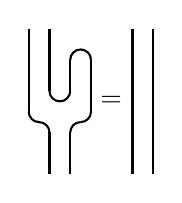
\begin{tikzpicture}[x=0.75pt,y=0.75pt,yscale=-0.5,xscale=0.5]
			%uncomment if require: \path (0,300); %set diagram left start at 0, and has height of 300
			
			%Shape: Arc [id:dp6748354158364842] 
			\draw  [draw opacity=0] (70,180) .. controls (70,180) and (70,180) .. (70,180) .. controls (70,180) and (70,180) .. (70,180) .. controls (70,185.52) and (65.52,190) .. (60,190) .. controls (54.48,190) and (50,185.52) .. (50,180) -- (60,180) -- cycle ; \draw   (70,180) .. controls (70,180) and (70,180) .. (70,180) .. controls (70,180) and (70,180) .. (70,180) .. controls (70,185.52) and (65.52,190) .. (60,190) .. controls (54.48,190) and (50,185.52) .. (50,180) ;  
			%Straight Lines [id:da30328109674550197] 
			\draw    (50,120) -- (50,180) ;
			%Straight Lines [id:da6276580027075187] 
			\draw    (70,150) -- (70,180) ;
			%Shape: Arc [id:dp8665893305935193] 
			\draw  [draw opacity=0] (70,150) .. controls (70,144.48) and (74.48,140) .. (80,140) .. controls (85.52,140) and (90,144.48) .. (90,150) -- (80,150) -- cycle ; \draw   (70,150) .. controls (70,144.48) and (74.48,140) .. (80,140) .. controls (85.52,140) and (90,144.48) .. (90,150) ;  
			%Straight Lines [id:da7863421858296449] 
			\draw    (90,150) -- (90,200) ;
			%Straight Lines [id:da3459195879084249] 
			\draw    (30,120) -- (30,200) ;
			%Shape: Arc [id:dp8748547741090917] 
			\draw  [draw opacity=0] (40,210) .. controls (40,210) and (40,210) .. (40,210) .. controls (40,210) and (40,210) .. (40,210) .. controls (34.48,210) and (30,205.52) .. (30,200) -- (40,200) -- cycle ; \draw   (40,210) .. controls (40,210) and (40,210) .. (40,210) .. controls (40,210) and (40,210) .. (40,210) .. controls (34.48,210) and (30,205.52) .. (30,200) ;  
			%Shape: Arc [id:dp1379517603769318] 
			\draw  [draw opacity=0] (40,210) .. controls (40,210) and (40,210) .. (40,210) .. controls (45.52,210) and (50,214.48) .. (50,220) -- (40,220) -- cycle ; \draw   (40,210) .. controls (40,210) and (40,210) .. (40,210) .. controls (45.52,210) and (50,214.48) .. (50,220) ;  
			%Straight Lines [id:da4885891795530013] 
			\draw    (50,220) -- (50,260) ;
			%Straight Lines [id:da9163027979285694] 
			\draw    (70,220) -- (70,260) ;
			%Shape: Arc [id:dp7957131684514858] 
			\draw  [draw opacity=0] (70,220) .. controls (70,214.48) and (74.48,210) .. (80,210) -- (80,220) -- cycle ; \draw   (70,220) .. controls (70,214.48) and (74.48,210) .. (80,210) ;  
			%Shape: Arc [id:dp9374819416671043] 
			\draw  [draw opacity=0] (90,200) .. controls (90,200) and (90,200) .. (90,200) .. controls (90,200) and (90,200) .. (90,200) .. controls (90,205.52) and (85.52,210) .. (80,210) -- (80,200) -- cycle ; \draw   (90,200) .. controls (90,200) and (90,200) .. (90,200) .. controls (90,200) and (90,200) .. (90,200) .. controls (90,205.52) and (85.52,210) .. (80,210) ;  
			%Straight Lines [id:da37935123830952877] 
			\draw    (130,120) -- (130,260) ;
			%Straight Lines [id:da5449144780510815] 
			\draw    (150,120) -- (150,260) ;
			
%			% Text Node
%			\draw (118,122) node [anchor=north west][inner sep=0.75pt]   [align=left] {$\displaystyle F$};
%			% Text Node
%			\draw (151,122) node [anchor=north west][inner sep=0.75pt]   [align=left] {$\displaystyle G$};
%			% Text Node
%			\draw (18,122) node [anchor=north west][inner sep=0.75pt]   [align=left] {$\displaystyle F$};
%			% Text Node
%			\draw (51,122) node [anchor=north west][inner sep=0.75pt]   [align=left] {$\displaystyle G$};
			% Text Node
			\draw (96,182) node [anchor=north west][inner sep=0.75pt]   [align=left] {$\displaystyle =$};
		\end{tikzpicture}\hspace{5em}	
		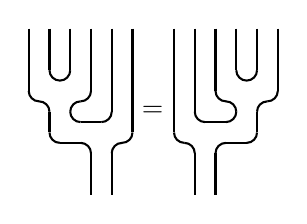
\begin{tikzpicture}[x=0.75pt,y=0.75pt,yscale=-0.5,xscale=0.5]
			%uncomment if require: \path (0,300); %set diagram left start at 0, and has height of 300
			
			%Straight Lines [id:da23613834151160362] 
			\draw    (60,110) -- (60,170) ;
			%Straight Lines [id:da9604875201085867] 
			\draw    (80,110) -- (80,150) ;
			%Straight Lines [id:da5764239342985473] 
			\draw    (100,110) -- (100,150) ;
			%Shape: Arc [id:dp2287987043326274] 
			\draw  [draw opacity=0] (100,150) .. controls (100,150) and (100,150) .. (100,150) .. controls (100,150) and (100,150) .. (100,150) .. controls (100,155.52) and (95.52,160) .. (90,160) .. controls (84.48,160) and (80,155.52) .. (80,150) -- (90,150) -- cycle ; \draw   (100,150) .. controls (100,150) and (100,150) .. (100,150) .. controls (100,150) and (100,150) .. (100,150) .. controls (100,155.52) and (95.52,160) .. (90,160) .. controls (84.48,160) and (80,155.52) .. (80,150) ;  
			%Shape: Arc [id:dp7721100718238127] 
			\draw  [draw opacity=0] (70,180) .. controls (70,180) and (70,180) .. (70,180) .. controls (70,180) and (70,180) .. (70,180) .. controls (64.48,180) and (60,175.52) .. (60,170) -- (70,170) -- cycle ; \draw   (70,180) .. controls (70,180) and (70,180) .. (70,180) .. controls (70,180) and (70,180) .. (70,180) .. controls (64.48,180) and (60,175.52) .. (60,170) ;  
			%Shape: Arc [id:dp9407575809888729] 
			\draw  [draw opacity=0] (70,180) .. controls (70,180) and (70,180) .. (70,180) .. controls (75.52,180) and (80,184.48) .. (80,190) -- (70,190) -- cycle ; \draw   (70,180) .. controls (70,180) and (70,180) .. (70,180) .. controls (75.52,180) and (80,184.48) .. (80,190) ;  
			%Shape: Arc [id:dp6454565332414952] 
			\draw  [draw opacity=0] (100,190) .. controls (100,184.48) and (104.48,180) .. (110,180) -- (110,190) -- cycle ; \draw   (100,190) .. controls (100,184.48) and (104.48,180) .. (110,180) ;  
			%Shape: Arc [id:dp8673772468248326] 
			\draw  [draw opacity=0] (120,170) .. controls (120,170) and (120,170) .. (120,170) .. controls (120,170) and (120,170) .. (120,170) .. controls (120,175.52) and (115.52,180) .. (110,180) -- (110,170) -- cycle ; \draw   (120,170) .. controls (120,170) and (120,170) .. (120,170) .. controls (120,170) and (120,170) .. (120,170) .. controls (120,175.52) and (115.52,180) .. (110,180) ;  
			%Shape: Arc [id:dp2598241437990816] 
			\draw  [draw opacity=0] (90,220) .. controls (90,220) and (90,220) .. (90,220) .. controls (90,220) and (90,220) .. (90,220) .. controls (84.48,220) and (80,215.52) .. (80,210) -- (90,210) -- cycle ; \draw   (90,220) .. controls (90,220) and (90,220) .. (90,220) .. controls (90,220) and (90,220) .. (90,220) .. controls (84.48,220) and (80,215.52) .. (80,210) ;  
			%Shape: Arc [id:dp544256142462509] 
			\draw  [draw opacity=0] (110,220) .. controls (110,220) and (110,220) .. (110,220) .. controls (115.52,220) and (120,224.48) .. (120,230) -- (110,230) -- cycle ; \draw   (110,220) .. controls (110,220) and (110,220) .. (110,220) .. controls (115.52,220) and (120,224.48) .. (120,230) ;  
			%Straight Lines [id:da8903362260377092] 
			\draw    (120,110) -- (120,170) ;
			%Straight Lines [id:da7438160797901054] 
			\draw    (140,110) -- (140,190) ;
			%Straight Lines [id:da03724352459412028] 
			\draw    (160,110) -- (160,210) ;
			%Shape: Arc [id:dp9831488201521568] 
			\draw  [draw opacity=0] (110,200) .. controls (110,200) and (110,200) .. (110,200) .. controls (110,200) and (110,200) .. (110,200) .. controls (104.48,200) and (100,195.52) .. (100,190) -- (110,190) -- cycle ; \draw   (110,200) .. controls (110,200) and (110,200) .. (110,200) .. controls (110,200) and (110,200) .. (110,200) .. controls (104.48,200) and (100,195.52) .. (100,190) ;  
			%Straight Lines [id:da05884826487291028] 
			\draw    (110,200) -- (130,200) ;
			%Shape: Arc [id:dp9170131358019777] 
			\draw  [draw opacity=0] (140,190) .. controls (140,190) and (140,190) .. (140,190) .. controls (140,190) and (140,190) .. (140,190) .. controls (140,195.52) and (135.52,200) .. (130,200) -- (130,190) -- cycle ; \draw   (140,190) .. controls (140,190) and (140,190) .. (140,190) .. controls (140,190) and (140,190) .. (140,190) .. controls (140,195.52) and (135.52,200) .. (130,200) ;  
			%Straight Lines [id:da3690258778575557] 
			\draw    (80,190) -- (80,210) ;
			%Straight Lines [id:da6476490596841975] 
			\draw    (90,220) -- (110,220) ;
			%Shape: Arc [id:dp2534445747495919] 
			\draw  [draw opacity=0] (160,210) .. controls (160,210) and (160,210) .. (160,210) .. controls (160,210) and (160,210) .. (160,210) .. controls (160,215.52) and (155.52,220) .. (150,220) -- (150,210) -- cycle ; \draw   (160,210) .. controls (160,210) and (160,210) .. (160,210) .. controls (160,210) and (160,210) .. (160,210) .. controls (160,215.52) and (155.52,220) .. (150,220) ;  
			%Shape: Arc [id:dp2618365391702757] 
			\draw  [draw opacity=0] (140,230) .. controls (140,224.48) and (144.48,220) .. (150,220) -- (150,230) -- cycle ; \draw   (140,230) .. controls (140,224.48) and (144.48,220) .. (150,220) ;  
			%Straight Lines [id:da36204815454282646] 
			\draw    (120,230) -- (120,270) ;
			%Straight Lines [id:da4578878839800886] 
			\draw    (140,230) -- (140,270) ;
			%Straight Lines [id:da07342481946917778] 
			\draw    (300,110) -- (300,170) ;
			%Straight Lines [id:da4757244672529106] 
			\draw    (280,110) -- (280,150) ;
			%Straight Lines [id:da4235497747706327] 
			\draw    (260,110) -- (260,150) ;
			%Shape: Arc [id:dp40270286179170967] 
			\draw  [draw opacity=0] (260,150) .. controls (260,150) and (260,150) .. (260,150) .. controls (260,150) and (260,150) .. (260,150) .. controls (260,155.52) and (264.48,160) .. (270,160) .. controls (275.52,160) and (280,155.52) .. (280,150) -- (270,150) -- cycle ; \draw   (260,150) .. controls (260,150) and (260,150) .. (260,150) .. controls (260,150) and (260,150) .. (260,150) .. controls (260,155.52) and (264.48,160) .. (270,160) .. controls (275.52,160) and (280,155.52) .. (280,150) ;  
			%Shape: Arc [id:dp09165014142522976] 
			\draw  [draw opacity=0] (290,180) .. controls (290,180) and (290,180) .. (290,180) .. controls (290,180) and (290,180) .. (290,180) .. controls (295.52,180) and (300,175.52) .. (300,170) -- (290,170) -- cycle ; \draw   (290,180) .. controls (290,180) and (290,180) .. (290,180) .. controls (290,180) and (290,180) .. (290,180) .. controls (295.52,180) and (300,175.52) .. (300,170) ;  
			%Shape: Arc [id:dp5864275574018558] 
			\draw  [draw opacity=0] (290,180) .. controls (290,180) and (290,180) .. (290,180) .. controls (284.48,180) and (280,184.48) .. (280,190) -- (290,190) -- cycle ; \draw   (290,180) .. controls (290,180) and (290,180) .. (290,180) .. controls (284.48,180) and (280,184.48) .. (280,190) ;  
			%Shape: Arc [id:dp5344581648323541] 
			\draw  [draw opacity=0] (260,190) .. controls (260,184.48) and (255.52,180) .. (250,180) -- (250,190) -- cycle ; \draw   (260,190) .. controls (260,184.48) and (255.52,180) .. (250,180) ;  
			%Shape: Arc [id:dp9129836518752186] 
			\draw  [draw opacity=0] (240,170) .. controls (240,170) and (240,170) .. (240,170) .. controls (240,170) and (240,170) .. (240,170) .. controls (240,175.52) and (244.48,180) .. (250,180) -- (250,170) -- cycle ; \draw   (240,170) .. controls (240,170) and (240,170) .. (240,170) .. controls (240,170) and (240,170) .. (240,170) .. controls (240,175.52) and (244.48,180) .. (250,180) ;  
			%Shape: Arc [id:dp16629270276658215] 
			\draw  [draw opacity=0] (270,220) .. controls (270,220) and (270,220) .. (270,220) .. controls (270,220) and (270,220) .. (270,220) .. controls (275.52,220) and (280,215.52) .. (280,210) -- (270,210) -- cycle ; \draw   (270,220) .. controls (270,220) and (270,220) .. (270,220) .. controls (270,220) and (270,220) .. (270,220) .. controls (275.52,220) and (280,215.52) .. (280,210) ;  
			%Shape: Arc [id:dp7129929613687838] 
			\draw  [draw opacity=0] (250,220) .. controls (250,220) and (250,220) .. (250,220) .. controls (244.48,220) and (240,224.48) .. (240,230) -- (250,230) -- cycle ; \draw   (250,220) .. controls (250,220) and (250,220) .. (250,220) .. controls (244.48,220) and (240,224.48) .. (240,230) ;  
			%Straight Lines [id:da40396451740325046] 
			\draw    (240,110) -- (240,170) ;
			%Straight Lines [id:da7773248064662102] 
			\draw    (220,110) -- (220,190) ;
			%Straight Lines [id:da29936944563790013] 
			\draw    (200,110) -- (200,210) ;
			%Shape: Arc [id:dp8203787022969811] 
			\draw  [draw opacity=0] (250,200) .. controls (250,200) and (250,200) .. (250,200) .. controls (250,200) and (250,200) .. (250,200) .. controls (255.52,200) and (260,195.52) .. (260,190) -- (250,190) -- cycle ; \draw   (250,200) .. controls (250,200) and (250,200) .. (250,200) .. controls (250,200) and (250,200) .. (250,200) .. controls (255.52,200) and (260,195.52) .. (260,190) ;  
			%Straight Lines [id:da05810339025763622] 
			\draw    (250,200) -- (230,200) ;
			%Shape: Arc [id:dp6061241961744019] 
			\draw  [draw opacity=0] (220,190) .. controls (220,190) and (220,190) .. (220,190) .. controls (220,190) and (220,190) .. (220,190) .. controls (220,195.52) and (224.48,200) .. (230,200) -- (230,190) -- cycle ; \draw   (220,190) .. controls (220,190) and (220,190) .. (220,190) .. controls (220,190) and (220,190) .. (220,190) .. controls (220,195.52) and (224.48,200) .. (230,200) ;  
			%Straight Lines [id:da15539630606768684] 
			\draw    (280,190) -- (280,210) ;
			%Straight Lines [id:da4663847440503588] 
			\draw    (270,220) -- (250,220) ;
			%Shape: Arc [id:dp766835997294987] 
			\draw  [draw opacity=0] (200,210) .. controls (200,210) and (200,210) .. (200,210) .. controls (200,210) and (200,210) .. (200,210) .. controls (200,215.52) and (204.48,220) .. (210,220) -- (210,210) -- cycle ; \draw   (200,210) .. controls (200,210) and (200,210) .. (200,210) .. controls (200,210) and (200,210) .. (200,210) .. controls (200,215.52) and (204.48,220) .. (210,220) ;  
			%Shape: Arc [id:dp3852774880550862] 
			\draw  [draw opacity=0] (220,230) .. controls (220,224.48) and (215.52,220) .. (210,220) -- (210,230) -- cycle ; \draw   (220,230) .. controls (220,224.48) and (215.52,220) .. (210,220) ;  
			%Straight Lines [id:da865092931126576] 
			\draw    (240,230) -- (240,270) ;
			%Straight Lines [id:da5959752980974766] 
			\draw    (220,230) -- (220,270) ;
			
			% Text Node
			\draw (166,182) node [anchor=north west][inner sep=0.75pt]   [align=left] {$\displaystyle =$};
			
			
		\end{tikzpicture}
	\end{center}
\end{proof}

\begin{definition}
    [label={monad-T-algebra}]
    {(单子的代数, 余单子的余代数)}
    设 $T$ 是范畴 $\mathcal C$ 上的单子.
    定义范畴 $\mathcal C$ 上的 \emph{$T$-代数}为 $\mathcal C$ 的对象 $c$ 配备一个态射 $h \colon Tc \to c$,
    满足如下交换图.
    \[
    \begin{tikzcd}[ampersand replacement=\&]
    	{T^2c} \& Tc \& c \& Tc \\
    	Tc \& c \&\& c
    	\arrow["Th", from=1-1, to=1-2]
    	\arrow["{\mu_c}"', from=1-1, to=2-1]
    	\arrow["h"', from=2-1, to=2-2]
    	\arrow["h", from=1-2, to=2-2]
    	\arrow["h", from=1-4, to=2-4]
    	\arrow["{\operatorname{id}_c}"', from=1-3, to=2-4]
    	\arrow["{\eta_c}", from=1-3, to=1-4]
    \end{tikzcd}
    \]
    $\mathcal C$ 上两个 $T$-代数之间的态射即是 $\mathcal C$ 中保持上述交换图的态射.
    记 $\mathcal C$ 上 $T$-代数的范畴为 $\mathcal C^{T}$, 这个范畴又称为 $T$ 的 \emph{Eilenberg--Moore 范畴}.
    
    对偶地, 设 $S$ 是范畴 $\mathcal C$ 上的余单子, 定义 $S$-\emph{余代数} (coalgebra) 是 $\mathcal C$ 的对象 $c$ 配备一个态射 $h\colon c\to Sc$,
    满足如下交换图.
    \[
    \begin{tikzcd}[ampersand replacement=\&]
    	{c} \& Sc \& c \& Sc \\
    	Sc \& {S^2c} \&\& c
    	\arrow["h", from=1-1, to=1-2]
    	\arrow["{h}"', from=1-1, to=2-1]
    	\arrow["Sh"', from=2-1, to=2-2]
    	\arrow["{\delta_c}", from=1-2, to=2-2]
    	\arrow["\rho_c", from=1-4, to=2-4]
    	\arrow["{\operatorname{id}_c}"', from=1-3, to=2-4]
    	\arrow["{h}", from=1-3, to=1-4]
    \end{tikzcd}
    \]
\end{definition}


\begin{prop}
	{($T$-代数的自由--遗忘伴随)}
	设 $T$ 是范畴 $\mathcal C$ 上的单子, 则有如下伴随:
	\[\begin{tikzcd}[ampersand replacement=\&]
		{\mathcal C} \& {\mathcal C^T,}
		\arrow[""{name=0, anchor=center, inner sep=0}, "{\text{自由}}", shift left=2, from=1-1, to=1-2]
		\arrow[""{name=1, anchor=center, inner sep=0}, "\text{遗忘}", shift left=2, from=1-2, to=1-1]
		\arrow["\dashv"{anchor=center, rotate=-90}, draw=none, from=0, to=1]
	\end{tikzcd}\]
	其中自由函子将 $c$ 对应到 $(Tc,\mu_c\colon T^2c\to Tc)$,
	遗忘函子将 $(c,h\colon Tc\to c)$ 对应到 $c$.
\end{prop}

\begin{propdef}
    {(比较函子)}
    在伴随产生的单子 (命题 \ref{monad-from-adjoint}) 中, 存在 $\mathcal D$ 到 $T$-代数范畴的\emph{比较函子} (comparison functor) $K\colon \mathcal D\to\mathcal C^T$,
    将对象 $d$ 对应到 $T$-代数 $Gd$, 其 $T$-代数结构为
    $$
    TGd=GFGd\overset{G\epsilon}{\longrightarrow}Gd.
    $$
\end{propdef}

\begin{example}
    {(集合与 $M$-集合之间的自由--遗忘伴随)}
    设 $M$ 是 (集合范畴 $\mathsf {Set}$ 中的) 幺半群, 那么 $T \colon X \mapsto M\times X$ 给出了集合范畴上的一个单子,
    自然变换 $\mu \colon T^2 \to T$ 由 $M$ 的乘法 $M\times M \to M$ 给出. 定义 \ref{monad-definition} 中的交换图对应 $M$ 的结合律和左右单位律.

    记 $\mathsf BM$ 为带有 $M$-作用的集合的范畴, 那么 $\mathsf {Set}$ 与 $\mathsf BM$ 之间有如下的伴随, 其中 ``自由'' 函子将集合 $X$ 对应到 $M\times X$.
    % https://q.uiver.app/#q=WzAsMixbMCwwLCJcXG1hdGhzZiB7U2V0fSJdLFsxLDAsIlxcbWF0aHNmIEJNIl0sWzAsMSwiXFx0ZXh0e+iHqueUsX0iLDAseyJvZmZzZXQiOi0yfV0sWzEsMCwiXFx0ZXh0e+mBl+W/mH0iLDAseyJvZmZzZXQiOi0yfV0sWzIsMywiIiwwLHsibGV2ZWwiOjEsInN0eWxlIjp7Im5hbWUiOiJhZGp1bmN0aW9uIn19XV0=
    \[\begin{tikzcd}[ampersand replacement=\&]
    	{\mathsf {Set}} \& {\mathsf BM}
    	\arrow[""{name=0, anchor=center, inner sep=0}, "{\text{自由}}", shift left=2, from=1-1, to=1-2]
    	\arrow[""{name=1, anchor=center, inner sep=0}, "{\text{遗忘}}", shift left=2, from=1-2, to=1-1]
    	\arrow["\dashv"{anchor=center, rotate=-90}, draw=none, from=0, to=1]
    \end{tikzcd}\]
    单子 $T$ 正是这对伴随由命题 \ref{monad-from-adjoint} 给出的单子 ``$\text{遗忘}\circ \text{自由}$''.
    
    此时, 一个 $T$-代数 $(X,h)$ 即为一个带有 $M$-作用的集合, $h \colon M\times X \to X$ 为 $M$-作用, 而定义 \ref{monad-T-algebra} 中的交换图则对应 $M$-作用的结合律和单位律.
    因此, 比较函子 $K\colon \mathsf BM\to \mathsf {Set}^T$ 是范畴的同构.
\end{example}

\begin{example}
    {(集合与幺半群之间的自由--遗忘伴随)}
    以 $\mathsf {Mon}$ 表示幺半群范畴,
    那么集合范畴 $\mathsf {Set}$ 与 $\mathsf {Mon}$ 之间存在伴随
    % https://q.uiver.app/#q=WzAsMixbMCwwLCJcXG1hdGhzZiB7U2V0fSJdLFsxLDAsIlxcbWF0aHNmIHtNb259Il0sWzAsMSwiXFx0ZXh0e+iHqueUsX0iLDAseyJvZmZzZXQiOi0yfV0sWzEsMCwiXFx0ZXh0e+mBl+W/mH0iLDAseyJvZmZzZXQiOi0yfV0sWzIsMywiIiwwLHsibGV2ZWwiOjEsInN0eWxlIjp7Im5hbWUiOiJhZGp1bmN0aW9uIn19XV0=
\[\begin{tikzcd}[ampersand replacement=\&]
	{\mathsf {Set}} \& {\mathsf {Mon}.}
	\arrow[""{name=0, anchor=center, inner sep=0}, "{\text{自由}}", shift left=2, from=1-1, to=1-2]
	\arrow[""{name=1, anchor=center, inner sep=0}, "{\text{遗忘}}", shift left=2, from=1-2, to=1-1]
	\arrow["\dashv"{anchor=center, rotate=-90}, draw=none, from=0, to=1]
\end{tikzcd}\]
    这对伴随给出的单子 $T= \text{遗忘}\circ \text{自由}\colon \mathsf {Set}\to\mathsf {Set}$ 将集合 $X$ 对应到 $X$ 生成的自由幺半群的底层集合
    $$TX=\coprod_{n\geq 0} X^n,$$
    也即 $X$ 上列表的集合.
    自然变换 $\mu\colon T^2\to T$ 将 ``列表的列表'' 拼接起来变为一个列表.
    一个 $T$-代数 $X$ 即为一个幺半群. 比较函子 $K\colon \mathsf {Mon} \to\mathsf {Set}^T$ 恰好也是范畴的同构.
\end{example}

\begin{example}
	[label={change-of-rings}]
	{(环的变换)}
	设 $A\to B$ 是交换环的同态, 则有伴随
	% https://q.uiver.app/#q=WzAsMixbMCwwLCJBXFxtYXRoc2Yge01vZH0iXSxbMSwwLCJCXFxtYXRoc2Yge01vZH0iXSxbMCwxLCIoLSlcXG90aW1lc19BIEIiLDAseyJvZmZzZXQiOi0yfV0sWzEsMCwiXFx0ZXh0e+mBl+W/mH0iLDAseyJvZmZzZXQiOi0yfV0sWzIsMywiIiwwLHsibGV2ZWwiOjEsInN0eWxlIjp7Im5hbWUiOiJhZGp1bmN0aW9uIn19XV0=
	\[\begin{tikzcd}[ampersand replacement=\&]
		{A\mathsf {Mod}} \& {B\mathsf {Mod}.}
		\arrow[""{name=0, anchor=center, inner sep=0}, "{(-)\otimes_A B}", shift left=2, from=1-1, to=1-2]
		\arrow[""{name=1, anchor=center, inner sep=0}, "{\operatorname{Hom}_B(B,-)}", shift left=2, from=1-2, to=1-1]
		\arrow["\dashv"{anchor=center, rotate=-90}, draw=none, from=0, to=1]
	\end{tikzcd}\]
	其中 $\operatorname{Hom}_B(B,-)$ 相当于将 $B$-模通过同态 $A\to B$ 视为 $A$ 模. 上述伴随是一般双模的张量--同态伴随的特例 (参考命题 \ref{group-action-tensor-hom}).
	它给出
	\begin{itemize}
		\item $A\mathsf {Mod}$ 上的单子 $(T,\eta,\mu)$, $T = (-)\otimes_A B$,
		$\eta_N \colon N\to N\otimes_A B, x\mapsto x\otimes 1$,
		$\mu_N \colon N\otimes_A B\otimes_A B \to N, x\otimes b\otimes b'\mapsto x\otimes bb'$;
		\item $B\mathsf {Mod}$ 上的余单子 $(S,\rho,\delta)$,
		$S = (-)\otimes_A B$,
		$\rho_M \colon M\otimes_A B\to M, x\otimes b\mapsto xb$,
		$\delta_M \colon M\otimes_A B \to M\otimes_A B\otimes_A B, x\otimes b\mapsto x\otimes 1\otimes b$.
%		$S$-余代数是 $B$-模 $M$ 配备一个同态 $h\colon M\to M\otimes_A B$, 满足
%		\todo{}
%		% https://q.uiver.app/#q=WzAsNCxbMCwwLCJNIl0sWzEsMCwiTVxcb3RpbWVzX0EgQiJdLFswLDEsIk1cXG90aW1lc19BIEIiXSxbMSwxLCJNXFxvdGltZXNfQSBCXFxvdGltZXNfQSBCIl0sWzAsMSwiaCJdLFswLDIsImgiLDJdLFsxLDMsIlxcZGVsdGFfTSJdLFsyLDNdXQ==
%		\[\begin{tikzcd}[ampersand replacement=\&]
%			M \& {M\otimes_A B} \\
%			{M\otimes_A B} \& {M\otimes_A B\otimes_A B}
%			\arrow["h", from=1-1, to=1-2]
%			\arrow["h"', from=1-1, to=2-1]
%			\arrow["{\delta_M}", from=1-2, to=2-2]
%			\arrow[from=2-1, to=2-2]
%		\end{tikzcd}\]
	\end{itemize}
	代数学著名教材 \cite{lww2} 的第 7 章介绍了这个单子的应用.
\end{example}
%
%\begin{example}
%	{(矩阵)}
%	固定含幺交换环 $R$.
%	对于集合 $B$, 
%\end{example}

\begin{example}
	[label={contravariant-power-set-self-adjunction}]
	{(反变幂集函子与其对偶函子的伴随)}
	反变幂集函子是指 $\mathsf {Set}$ 上的幂对象函子 $P\colon \mathsf {Set}^{\op} \to \mathsf {Set}$ (定义 \ref{power-object-functor}). 考虑其对偶 (即同一个函子, 不过所有箭头反向) $P^\op\colon \mathsf {Set}\to\mathsf {Set}^\op$. 自然同构 $\operatorname{Hom}_{\mathsf {Set}^\op}(P^\op Y,X) = \operatorname{Hom}_{\mathsf {Set}}(X,PY)\simeq \operatorname{Hom}_{\mathsf {Set}}(X\times Y,\Omega) \simeq \operatorname{Hom}_{\mathsf {Set}}(Y,PX)$ 表明有如下伴随.
	% https://q.uiver.app/#q=WzAsMixbMCwwLCJcXG1hdGhzZiB7U2V0fSJdLFsxLDAsIlxcbWF0aHNmIHtTZXR9Xlxcb3AiXSxbMCwxLCJQXlxcb3AiLDAseyJvZmZzZXQiOi0yfV0sWzEsMCwiUCIsMCx7Im9mZnNldCI6LTJ9XSxbMiwzLCIiLDAseyJsZXZlbCI6MSwic3R5bGUiOnsibmFtZSI6ImFkanVuY3Rpb24ifX1dXQ==
	\[\begin{tikzcd}[ampersand replacement=\&]
		{\mathsf {Set}} \& {\mathsf {Set}^\op}
		\arrow[""{name=0, anchor=center, inner sep=0}, "{P^\op}", shift left=2, from=1-1, to=1-2]
		\arrow[""{name=1, anchor=center, inner sep=0}, "P", shift left=2, from=1-2, to=1-1]
		\arrow["\dashv"{anchor=center, rotate=-90}, draw=none, from=0, to=1]
	\end{tikzcd}\]
	
	在代数--几何对偶 (参考 Stone 对偶, 命题 \ref{Stone-duality}) 之下, 集合作为 ``几何'' 对应的 ``代数'' 称为\emph{完备原子型 Boole 代数} (complete atomic Boolean algebra).
\end{example}

对于某些伴随产生的单子 $T$, 我们发现 $T$-代数的范畴恰好等价于伴随另一边的范畴; 因此这一对伴随可视为范畴 $\mathcal C$ 与其上的 $T$-代数范畴 $\mathcal C^T$ 之间的自由--遗忘伴随. 于是有如下的定义.

\begin{definition}
    {(单子性伴随)}
    设一对伴随函子
    % https://q.uiver.app/#q=WzAsMixbMCwwLCJcXG1hdGhzZiBDIl0sWzEsMCwiXFxtYXRoc2YgRCJdLFsxLDAsIkciLDAseyJvZmZzZXQiOi0yfV0sWzAsMSwiRiIsMCx7Im9mZnNldCI6LTJ9XSxbMywyLCIiLDAseyJsZXZlbCI6MSwic3R5bGUiOnsibmFtZSI6ImFkanVuY3Rpb24ifX1dXQ==
    $$
    \begin{tikzcd}[ampersand replacement=\&]
    	{\mathcal C} \& {\mathcal D}
    	\arrow[""{name=0, anchor=center, inner sep=0}, "G", shift left=2, from=1-2, to=1-1]
    	\arrow[""{name=1, anchor=center, inner sep=0}, "F", shift left=2, from=1-1, to=1-2]
    	\arrow["\dashv"{anchor=center, rotate=-90}, draw=none, from=1, to=0]
    \end{tikzcd}
    $$
    确定了一个单子 $T = GF \colon \mathcal C \to \mathcal C$.
    若比较函子 $K\colon \mathcal D\to\mathcal C^T$ 构成范畴等价, 则称这对伴随为\emph{单子性伴随} (monadic adjunction), 称右伴随 $G$ 为\emph{单子性函子}. 换言之, $G$ 可视为 $\mathcal C$ 上某个单子的代数范畴到 $\mathcal C$ 的遗忘函子.
\end{definition}

\begin{example}
	{}
	自反子范畴的嵌入 $i\colon \mathcal D\to\mathcal C$ 是单子性的; 也即 $\mathcal D$ 的对象可视为单子 $ia\colon \mathcal C\to\mathcal C$ 的代数.
\end{example}

\begin{example}
	{(平坦下降)}
	在例 \ref{change-of-rings} 中, 若 $B$ 是\emph{忠实平坦 $A$-代数} (即 $B\otimes_A{-}$ 是忠实函子且保持有限极限), 则伴随是单子性的.
\end{example}

% the Eilenberg-Moore category of ultrafilter monad is the category of compact Hausdorff spaces with its obvious forgetful functor to Set.




\section{万有代数}

\label{universal-algebra}

万有代数可视为群, 环, 模, Boole 代数等概念的共同推广, 又称\emph{等式逻辑} (equational logic), 是一阶逻辑的简单例子. 本节介绍 William Lawvere 1963 年的博士论文 \emph{Functorial Semantics of Algebraic Theories} 引入的研究万有代数的范畴论方法.

\subsection{Lawvere 理论}

\begin{definition}
	[label={Lawvere-theory}]
	{(Lawvere 理论)}
	一个\emph{Lawvere 理论}是一个保积函子 $\mathbb{N}^{\op}\to\mathbb T$ ($\mathbb{N}$ 是有限集 $0,1,2,\cdots$ 构成的 $\mathsf {Set}$ 的全子范畴), 在对象集上为双射. 我们将 $\mathbb{N}$ 的对象 $n$ 在这个函子下的像仍记为 $n$.
\end{definition}

Lawvere 理论将一个代数理论的运算记录在范畴 $T$ 的态射中, 态射 $n \to 1$ 为 $n$ 元运算. 例如在群的理论中, 乘法是一个态射 $2 \to 1$, 而取逆是一个态射 $1\to 1$.
Lawvere 理论对应的范畴 $\mathbb T$ 是一种 ``句法范畴'' (但与定义 \ref{first-order-theory-syntactic-category} 中的句法范畴尚有差距).

\begin{definition}
	{(Lawvere 理论的模型)}
	对于 Lawvere 理论 $\mathbb T$ 以及具有有限乘积的范畴 $\mathcal C$, 定义 $\mathbb T$ 在范畴 $\mathcal C$ 中的\emph{模型}为保积函子
	$$
	A \colon \mathbb T \to \mathcal {C},
	$$
	而模型之间的同态为保积函子之间的自然变换.
	称 $A(1)$ 为 $A$ 的\emph{底集} (underlying set).
	记 $\mathbb T$ 在 $\mathsf {Set}$ 中的模型的范畴为 $\mathbb T\mathsf {Mod}$.
\end{definition}

%\todo{代数理论的表现, Borceux 3.2.9}
\begin{definition}
	[label={presentation-of-an-algebraic-theory}]
	{(代数理论的表现)}
	一个 (单类型) \emph{代数理论的表现} (presentation of an algebraic theory) $\mathcal T$ 是如下资料,
	\begin{itemize}
		\item 任意多个\emph{变量};
		\item 一些\emph{运算符号}, 每一个运算符号对应一个固定的非负整数, 称为其\emph{元数} (arity);
		\item 一些\emph{公理}, 其中每个公理形如 $s=t$, $s,t$ 为\emph{项} (terms)\footnotemark{}, 而项的归纳定义如下:
		\begin{itemize}
			\item 每个变量是一项;
			\item 若 $f$ 是 $n$ 元运算符号, $t_1,\cdots,t_n$ 各是一项, 则 $f(t_1,\cdots,t_n)$ 是一项. (特别地, 每个零元运算是一项, 即一个常数.)
		\end{itemize}
	\end{itemize}
\end{definition}
\footnotetext{为了严谨, 我们应该补充说明: 对每一条公理 $s=t$, 改变 $s,t$ 中某个变量的名称仍是一条公理. 但这种事情是不重要的.}

\begin{remark}
	{}
	这里 ``代数理论的表现'' 须理解为一个整体术语. 它是定义 \ref{kinds-of-theories} 中的代数理论的特例, 其中只有一个类型. 此处这样称呼的理由是, 我们必须把它与 Lawvere 理论区分开. 后面我们将看到, 一个 ``代数理论的表现'' 唯一确定了一个 Lawvere 理论, 但后者的表现远远不是唯一的.
	例如群的理论可以仅由一种运算 $(a,b)\mapsto a^{-1} b$ 确定.
\end{remark}

\begin{definition}
	[label={model-of-presentation-of-Lawvere-theory}]
	{(``代数理论之表现'' 的模型)}
	设 $\mathcal T$ 是代数理论的表现 (定义 \ref{presentation-of-an-algebraic-theory}). 定义一个 \emph{$\mathcal T$-模型} $M$ 为如下资料:
	\begin{itemize}
		\item 集合 $M$ (称作该模型的\emph{底层集合}),
		\item 对每个非负整数 $n$ 以及 $n$ 元运算符号 $f$, 一个映射 $[[f]]\colon M^n\to M$;
	\end{itemize}
	满足所有的公理, 也即当 $\mathcal T$ 中的变量取值为 $M$ 的任何元素时, 公理 $s=t$ 的两端总是取相等的值. 其中, 一个项 $t$ 的取值 $[[t]]$ 归纳定义如下:
	\begin{itemize}
		\item 每个变量 $x$ 可取 $M$ 中任意的值, $[[x]]\in M$;
		\item 若 $f$ 是 $n$ 元运算符号, $t_1,\cdots,t_n$ 各是一项, 则 $f(t_1,\cdots,t_n)$ 的取值是 $[[f]]([[t_1]],\cdots, [[t_n]])$. (特别地, 每个零元运算取 $M$ 中一个固定的值.)
	\end{itemize}
	所有 $\mathcal T$-模型构成一个范畴 $\mathcal T\mathsf {Mod}$, 其中的态射为保持所有运算的映射.
\end{definition}

\begin{propdef}
	[label={finitely-generated-free-model}]
	{(有限生成自由模型)}
	设 $\mathcal T$ 为代数理论的表现, $n\geq 0$. 记 $T(n)$ 为其中仅涉及 $n$ 个变量 $x_1,\cdots,x_n$ 的项的集合. 在 $T(n)$ 上定义等价关系 $\sim$ 由如下条件生成:
	\begin{itemize}
		\item 对于公理 $s=t$, 有 $s\sim t$;
		\item 对于 $n$ 元运算符号 $f$, 若 $s_i\sim t_i\,(i=1,\cdots,n)$, 则有 $f(s_1,\cdots,s_n)\sim f(t_1,\cdots,t_n)$.
	\end{itemize}
	则商集 $F(n):=T(n)/{\sim}$ 是 \emph{$n$ 个元素生成的自由 $\mathcal T$-模型}, 也即对任意 $\mathcal T$-模型 $M$, 集合映射 $\{x_1,\cdots,x_n\}\to M$ 唯一地延拓为 $\mathcal T$-模型态射 $F(n)\to M$.
\end{propdef}

由上述命题, 对任意 $\mathcal T$-模型 $M$ 有自然同构
\[
\operatorname{Hom}_{\mathcal T\mathsf {Mod}}(F(n),M)\simeq \operatorname{Hom}_{\mathcal T\mathsf {Mod}}(F(1),M)^n.
\]
这表明 $F(n)$ 在范畴 $\mathcal T\mathsf {Mod}$ 中同构于 $n$ 个 $F(1)$ 的和. 特别地, $F(0)$ 是 $0$ 个对象的和, 也即 $\mathcal T\mathsf {Mod}$ 的始对象.

\begin{propdef}
	{(Lawvere 理论及其表现)}
	设 $\mathcal T$ 是代数理论的表现 (定义 \ref{presentation-of-an-algebraic-theory}). 那么 $\mathcal T\mathsf {Mod}$ 中由有限生成自由模型构成的全子范畴的对偶范畴构成一个 Lawvere 理论 $\mathbb T$, 且有范畴等价\[\mathcal T\mathsf {Mod} \simeq \mathbb T\mathsf {Mod}.\]
	此时称 $\mathcal T$ 为 $\mathbb T$ 的一个\emph{表现}.
\end{propdef}
\begin{proof}
	首先证明 $\mathbb T$ 为 Lawvere 理论.
	前面提到 $F(n)$ 在 $\mathcal T\mathsf {Mod}$ 中同构于 $n$ 个 $F(1)$ 的和, 因此 $F(n)$ 在 $\mathbb T$ 中同构于 $n$ 个 $F(1)$ 的积.
	
	给定保积函子 $A\colon \mathbb T\to\mathsf {Set}$, 我们构造一个 $\mathcal T$-模型 $M$ 如下.
	令底层集合 $M=A(F(1))$. 对 $\mathcal T$ 中每个 $n$ 元运算符号 $f$, 有一个元素 $[f(x_1,\cdots,x_n)]\in F(n)$ (方括号表示 $\sim$-等价类), 对应一个 $\mathcal T$-模型态射 $\bar{f}\colon F(1)\to F(n)$, 即对偶范畴 $\mathbb T$ 中的态射 $F(n)\to F(1)$. 而 $A$ 为保积函子, 故 $M^n\simeq A(F(n))$. 定义
	$$
	\interpretation{f} := A(\bar f)\colon M^n\simeq A(F(n)) \to A(F(1)) = M.
	$$
	下面说明 $M$ 是 $\mathcal T$-模型.
	对每条公理 $s=t$ (其中仅含有变量 $x_1,\cdots,x_n$),
	由 $\sim$ 的定义有 $[s]=[t]\in F(n)$, 从而有 $\bar s = \bar t\colon F(1)\to F(n)$, $\interpretation{s}=\interpretation{t}\colon M^n\to M$.
	
	反之, 给定 $\mathcal T$-模型 $M$, 我们构造保积函子 $A\colon \mathbb T\to\mathsf {Set}$.
	令 $A(F(n)) = M^n$, 由积的性质我们只需要指定态射 $F(n)\to F(1)$ 对应的映射 $M^n\to M$.
	而态射 $F(n)\to F(1)$ 等同于变量 $x_1,\cdots,x_n$ 构成的一个项 (的等价类) $[t]\in F(n)$, 项的取值 $(\interpretation{x_1},\cdots,\interpretation{x_n})\mapsto \interpretation{t}$ 便给出了映射 $M^n\to M$. 由 $\interpretation{-}$ 的定义, 这确实给出了一个函子 $\mathbb T\to\mathsf {Set}$.
	
	容易说明如上构造的函子性. 它们给出了范畴等价 $\mathcal T\mathsf {Mod} \simeq \mathbb T\mathsf {Mod}$.
\end{proof}

\begin{example}
	{}
	一个 Lawvere 理论 $\mathbb T$ 有一种 ``极大'' 的表现 $\mathcal T$, 即所有 $\operatorname{Hom}_{\mathbb T}(n,1)$ 的元素都是一个 $n$ 元运算符号, 所有态射之间的等式都是一条公理. 很明显, 此时有 $\mathcal T\mathsf {Mod}\simeq\mathbb T\mathsf {Mod}$ (因为此时定义 \ref{model-of-presentation-of-Lawvere-theory} 所要求的正是保积函子的定义).
\end{example}

%需要注意的是, 一个 ``代数理论的表现'' $\mathcal T$ 唯一确定了一个 Lawvere 理论, 而一个 Lawvere 理论对应的表现远不是唯一的.

\begin{example}
	{(群的 Lawvere 理论)}
	群的 Lawvere 理论 $\mathbb T_{\text{Grp}}$ 由二元运算 $m$, 一元运算 $i$, 零元运算 $e$ 以及三者满足的关系所表现.
	定义 $F(n)$ 为 $n$ 个元素生成的自由群, $\mathbb T_{\text{Grp}}$ 为所有 $F(n)$ 在 $\mathsf {Grp}$ 中构成的全子范畴的对偶范畴. 群范畴中 $F(n)$ 与 $F(m)$ 的余积 (群的自由积) 为 $F(n+m)$, 所以在 $\mathbb T_{\text{Grp}}$ 中有 $F(n) \simeq F(1)^n$.
	设 $A \colon \mathbb T_{\text{Grp}} \to \mathsf {Set}$ 为保积函子, 记 $G=A(F(1))$, 我们可以具体写出 $G$ 上的乘法映射:
	$$
	G\times G \simeq A(F(2)) \overset{A(m)}{\longrightarrow} A(F(1)) = G,
	$$
	其中群同态 $F(1) \to F(2)$ 将 $F(1)$ 的生成元映射到 $F(2)$ 两个生成元的乘积.
\end{example}

\begin{remark}
	[label={walking-model}]
	{(游走模型)}
	我们形象地称对象 $F(1)$ 为理论 $\mathbb T$ 的\emph{游走模型} (walking model), 因为理论 $\mathbb T$ 的任何模型都是 $F(1)$ 在相应范畴中的一个化身.
	例如对于群的理论 $\mathbb T_{\text{Grp}}$, 其在拓扑空间范畴 $\mathsf {Top}$ 中的模型 $\mathbb T_{\text{Grp}} \to \mathsf {Top}$ 即为拓扑群,
	在光滑流形范畴 $\mathsf {Man}$ 中的模型 $\mathbb T_{\text{Grp}} \to \mathsf {Man}$ 即为 Lie 群.
\end{remark}

\begin{example}
	{(格的 Lawvere 理论)}
	%\todo{Borceux 3.3.5d}
	格的 Lawvere 理论 $\mathbb T_{\text{Lat}}$ 由二元运算 $\land,\lor$ 以及如下关系所表现:
	\begin{align*}
		x\land (y\land z) &= (x\land y)\land z,&
		x\lor (y\lor z) &= (x\lor y)\lor z,\\
		x\land y &= y \land x, & x\lor y &= y \lor x,\\
		x\land x &= x, & x\lor x &= x,\\
		x\land (x\lor y) &= x, & x\lor (x\land y) &= x.
	\end{align*}
\end{example}

\begin{example}
	[label={R-mod-Lawvere-theory}]
	{($R$-模的 Lawvere 理论)}
	固定一个 ($\mathsf{Set}$ 中的) 环 $R$. $R$-模的 Lawvere 理论 $\mathbb T_{R\text{Mod}}$ 由二元运算 $+$, 每个元素 $r\in R$ 对应的一元运算 $\rho_r$ 以及对应每两个元素 $r,s$ 的如下关系所表现:
	\begin{align*}
		\rho_r(x+y) &= \rho_r(x) + \rho_r(y),\\
		\rho_r(\rho_s(x)) &= \rho_{rs}(x),\\
		\rho_{r+s}(x) &= \rho_{r}(x) + \rho_s(x).
	\end{align*}
	记 $R^n$ 为 $n$ 个元素生成的自由 $R$-模, 那么 $\mathbb T_{R\text{Mod}}$ 为所有 $R^n$ 在 $R\mathsf {Mod}$ 中构成的全子范畴的对偶范畴.
	$R\mathsf {Mod}$ 中 $R^n$ 与 $R^m$ 的余积为 $R^{n+m}$, 所以在 $\mathbb T_{R\text{Mod}}$ 中有 $R^n = (R^1)^n$.
	设 $A\colon \mathbb T_{R\text{Mod}} \to \mathsf {Set}$ 为保积函子,
	记 $M = A(R^1)$,
	则 $M$ 上的 $R$-模结构由如下资料给出:
	\[
	\begin{aligned}
		+\colon M\times M &\simeq A(R^2) \overset{A(+)}{\longrightarrow} A(R^1)\simeq M,
		\\
		\times r \colon M &\simeq A(R^1) \overset{A(\rho_r)}{\longrightarrow} A(R^1)\simeq M.
	\end{aligned}
	\]
\end{example}

\begin{example}
	{(平凡的 Lawvere 理论)}
	$\mathbb T = \mathbb N^{\op}$ 本身是一个 Lawvere 理论. $\mathbb T$ 在 $\mathcal C$ 中的模型等同于 $\mathcal C$ 的对象.
	该理论由 $0$ 个运算符号和 $0$ 个公理所表现.
	由于我们一般以集合范畴中模型的名称来命名一个 Lawvere 理论, 平凡的 Lawvere 理论也可称作 ``集合的 Lawvere 理论''.
\end{example}

\begin{example}
	[label={Lawvere-theory-CartSp}]
	{(光滑代数)}
	微分流形 $\mathbb{R}^n\,(n=0,1,2,\cdots)$ 构成的范畴 $\mathsf {CartSp}$ 是一个 Lawvere 理论.
	每个光滑映射 $f\colon \mathbb{R}^n\to \mathbb{R}$ 都对应这种代数结构中的一个 $n$ 元运算.
	例如这种代数结构至少要包含加法与乘法 $+,\times\colon \mathbb{R}^2\to \mathbb{R}$,
	包含所有实数 $\mathbb{R}^0\to\mathbb{R}$,
	还包含如 $\sin,\exp$ 等运算.
	
	Lawvere 理论 $\mathsf {CartSp}$ 的模型称作\emph{光滑代数}. 光滑流形上的函数代数 $C^\infty (M)$ 是最简单的光滑环, 而一些更广义的几何对象上的 ``函数代数'' 也构成光滑环, 如 ``无穷小线段上的函数代数'' $\mathbb{R}[x]/(x^2)$ 等.
\end{example}



\subsection{模型的表现}

给定一个 Lawvere 理论 $\mathbb T$, 我们描述如何用生成元和关系表现一个 $\mathbb T$-模型.
以 $F(n)$ 表示 $n$ 个元素生成的自由 $\mathbb T$-模型 (定义 \ref{finitely-generated-free-model}).
%\todo{}

\begin{definition}
	{(有限表现模型)}
	设 $A\colon \mathbb T\to\mathsf {Set}$ 是 $\mathbb T$-模型.
	若存在 $m,n$ 使得 $A$ 可表示为余等化子 $$A\simeq\operatorname{coeq}(s,t\colon F(m)\rightrightarrows F(n)),$$
	则称 $A$ 为\emph{有限表现} $\mathbb T$-模型; 具体地, $A$ 是由 $n$ 个生成元和 $m$ 个关系表现的 $\mathbb T$-模型, 此处每个关系是指一个等式 $s_i=t_i$, $s_i,t_i\in F(n)$, $1\leq i\leq m$.
\end{definition}

%态射 $F(m)\to F(n)$ 等同于 $m$ 个

有限表现群, 有限表现环, 有限表现 $R$-模, 有限表现 $R$-代数 ($R$ 为环) 等等概念均为上述概念的特例.

\begin{prop}
	{(有限表现的等价定义)}
	有限表现 $\mathbb T$-模型等价于范畴 $\mathbb T\mathsf {Mod}$ 中的有限表现对象 (定义 \ref{lambda-presentable-objects}); 换言之,
	$\mathbb T$-模型 $A\colon \mathbb T\to\mathsf {Set}$ 有限表现当且仅当
	$\operatorname{Hom}_{\mathbb T\mathsf {Mod}}(A,-)$ 保持滤余极限.
\end{prop}

\begin{proof}
	~
	\begin{itemize}
		\item 设 $A\simeq\operatorname{coeq}(s,t\colon F(m)\rightrightarrows F(n))$,
		则有自然同构
		$$
			\begin{aligned}
				\operatorname{Hom}_{\mathbb T\mathsf {Mod}}(A,B)
				&\simeq
				\operatorname{eq}
				\big({
					\operatorname{Hom}_{\mathbb T\mathsf {Mod}}(F(n),B) \rightrightarrows \operatorname{Hom}_{\mathbb T\mathsf {Mod}}(F(m),B)
				}\big)
				\\&\simeq
				\operatorname{eq}
				\big({
					B^n \rightrightarrows B^m
				}\big)
			\end{aligned}
		$$
		而集合的滤余极限与有限极限交换 (命题 \ref{lambda-filtered-colimit-commutes-with-lambda-small-limit}), 故 $\operatorname{Hom}(A,-)$ 保持滤余极限.
		\item 设 $\operatorname{Hom}(A,-)$ 保持滤余极限. 与例 \ref{lambda-presentable-group} 中的证明完全类似, 考虑
		\[
		I:=\{B\leq A\mid \text{$B$ 由有限个元素生成}\},
		\]
		那么 $A = \operatorname{colim}_{B\in I}B$, 从而 $\operatorname{id}_A$ 穿过某个同态 $B\hookrightarrow A$, $A$ 可由有限个元素生成.
		%
		进一步, 设 $F$ 为有限生成自由 $\mathbb T$-模型, 且有满同态 $\varphi\colon F\to A$ (这里是指底层集合上为满射).
		令
		\[
		J := \big\{ K={F/{\sim}} \bigm| \text{$\sim$ 由 $\ker\varphi$ 中有限个元素生成} \big\},
		\]
		容易说明 $A=\operatorname{colim}_{K\in J}K$, 其中每个 $K$ 到 $A$ 有典范的满同态.
		那么 $\operatorname{id}_A$ 穿过某个同态 $K\to A$, 说明 $A$ 可由有限个生成元和有限个关系所表现.
	\end{itemize}
\end{proof}


\subsection{代数理论之间的态射}

所有 Lawvere 理论构成一个范畴. 我们将看到 Lawvere 理论之间的态射体现了不同代数结构之间的关系.

\begin{definition}
	{(Lawvere 理论之间的态射)}
	设 $\mathbb T_1$, $\mathbb T_2$ 为 Lawvere 理论.
	定义 Lawvere 理论之间的态射 $\mathbb T_1 \to \mathbb T_2$ 为保持乘积且将 $1$ 映射为 $1$ 的函子.
	如此所有 Lawvere 理论构成范畴 $\mathsf {Law}$.
\end{definition}

Lawvere 理论之间的态射 $f\colon \mathbb T_1 \to \mathbb T_2$ 可理解为将 $\mathbb T_2$ 的游走模型视为 $\mathbb T_1$-模型的方法. 由此我们可将任意范畴中的 $\mathbb T_2$-模型转化为 $\mathbb T_1$-模型.
特别地, 有函子 $f^*\colon \mathbb T_2\mathsf {Mod} \to \mathbb T_1\mathsf {Mod}$, 它正是与 $f$ 的复合.

\begin{example}
	[label={lawvere-theory-morphisms}]
	{(常见的 Lawvere 理论态射)}
	\begin{enumerate}[(1)]
		\item 集合的 Lawvere 理论 $\mathbb N^{\op}$ 是 $\mathsf {Law}$ 的始对象, 对应遗忘函子 $\mathbb T\mathsf {Mod} \to \mathsf {Set}$.
		\item 幺半群的 Lawvere 理论到群的 Lawvere 理论有态射 $\mathbb T_{\text{Mon}}  \to \mathbb T_{\text{Grp}}$, 对应遗忘函子 $\mathsf {Grp}\to\mathsf {Mon}$.
		根据注 \ref{walking-model}, 我们称 ``游走的群是一个幺半群''. 既然游走的群是幺半群, 那么所有的群便都是幺半群.
		\item Abel 群的 Lawvere 理论到环的 Lawvere 理论有态射 $\mathbb T_{\text{Ab}}  \to \mathbb T_{\text{Ring}}$, 对应遗忘函子 $\mathsf {Ring}\to\mathsf {Ab}$, ``取加法群''. 根据注 \ref{walking-model}, 我们称 ``游走的环是一个 (加法) 群''.
		\item 幺半群的 Lawvere 理论到环的 Lawvere 理论有态射 $\mathbb T_{\text{Mon}}  \to \mathbb T_{\text{Ring}}$, 对应遗忘函子 $\mathsf {Ring}\to\mathsf {Mon}$, ``取乘法幺半群''.
		\item 固定一个域 $k$, 由 $k$ 上的结合代数 $A$ 可得一个 Lie 代数, 其 Lie 括号为 $[a,b] = ab-ba$. 这给出了 $k$ 上的 Lie 代数的 Lawvere 理论到 (结合) 代数的 Lawvere 理论的态射 $\mathbb T_{\text{Lie}}  \to \mathbb T_{\text{Alg}}$, 对应函子 $\mathsf {Alg}_k \to \mathsf {Lie}_k$.
		\item 环同态 $f\colon R\to S$ 给出 Lawvere 理论的态射 $f\colon \mathbb T_{R\text{Mod}} \to \mathbb T_{S\text{Mod}}$ ($\mathbb T_{R\text{Mod}}$ 的定义见 \ref{R-mod-Lawvere-theory}). 这对应 ``遗忘函子'' $S\mathsf {Mod} \to R\mathsf {Mod}$.
		\item $\mathbb{R}$-代数的 Lawvere 理论到光滑代数的 Lawvere 理论有态射 $\mathbb T_{\mathbb{R}\text{Alg}} \to \mathsf {CartSp}$,
		对应遗忘函子 $C^\infty \mathsf {Alg} \to \mathbb{R}\mathsf {Alg}$; ``光滑代数至少是一个 $\mathbb{R}$-代数'' (注 \ref{remark-smooth-algebra-R-algebra}).
	\end{enumerate}
\end{example}

\begin{prop}
	{}
	对于 Lawvere 理论之间的态射 $f\colon \mathbb T_1 \to \mathbb T_2$,
	函子 $f^*\colon \mathbb T_2\mathsf {Mod} \to \mathbb T_1\mathsf {Mod}$ 有左伴随 $f_!\colon \mathbb T_1\mathsf {Mod} \to \mathbb T_2\mathsf {Mod}$.
\end{prop}
\begin{proof}
	这个证明参考了 \cite{HCA2} 3.7.7.
	回忆 $f^*\colon \mathsf {Fun}(\mathbb T_2,\mathsf {Set}) \to \mathsf {Fun}(\mathbb T_1,\mathsf {Set})$ 有左伴随 $$f_!\colon \mathsf {Fun}(\mathbb T_1,\mathsf {Set}) \to \mathsf {Fun}(\mathbb T_2,\mathsf {Set}),$$ 它是沿 $f$ 的左 Kan 扩张 (例 \ref{presheaf-category-adjunction}),
	\[
		f_!(A)(n) = \operatorname{colim}_{m\to n} A(m),
	\]
	其中指标范畴由 $\mathbb T_2$ 中的态射 $m\to n$ ($m$ 跑遍 $0,1,2,\cdots$) 构成.
	我们要证明对于保积函子 $A\colon \mathbb T_1\to\mathsf {Set}$, 有 $f_!(A)$ 也是保积函子.
	注意由于 $\mathbb T_2$ 的对象 $n$ 是 $n$ 个 $1$ 的积, 故一个态射 $m\to n$ 等同于 $n$ 个态射 $m\to 1$.
	那么
	\[
		\begin{aligned}
			f_!(A)(n) &\simeq \operatorname{colim}_{m\to n} A(m) \\
			&\simeq \operatorname{colim}_{m\to 1,\cdots, m\to 1} A(m)\\
			&\simeq \big({\operatorname{colim}_{m\to 1} A(m)}\big)^n \simeq f_!(A)(1)^n.
		\end{aligned}
	\]
\end{proof}

上述构造的直观是, $f_!(A)$ 的底层集合 (即 $f_!(A)(1)$) 由所有形如 $\varphi(a_1,\cdots,a_m)$ 的项构成, 其中 $a_1,\cdots,a_m$ 是 $A$ 的底层集合 (即 $A(1)$) 的元素, $\varphi\colon m\to 1$ 是理论 $\mathbb T_2$ 中的 $m$ 元运算.

\begin{example}
	[label={algebraic-theory-morphism-example}]
	{}
	对于例 \ref{lawvere-theory-morphisms} 提到的每个态射 $f$, 我们来描述 $f_!$.
	\begin{enumerate}[(1)]
		\item $f\colon \mathbb N^{\op}\to\mathbb T$, $f_!\colon \mathsf {Set}\to\mathbb T\mathsf {Mod}$ 是 ``自由'' 函子.
		\item $f\colon \mathbb T_{\text{Mon}}  \to \mathbb T_{\text{Grp}}$, $f_!\colon \mathsf {Mon}\to\mathsf {Grp}$ 给出幺半群的 ``泛包络群'', 对于交换幺半群它是所谓 Grothendieck 群.
		\item $f\colon \mathbb T_{\text{Ab}}  \to \mathbb T_{\text{Ring}}$, $f_!\colon \mathsf {Ab}\to\mathsf {Ring}$ 给出 Abel 群 $A$ 的\emph{张量代数} $TA=\bigoplus_{n\geq 0} A^{\otimes n}$.
		\item $f\colon \mathbb T_{\text{Mon}}  \to \mathbb T_{\text{Ring}}$, $f_!\colon \mathsf {Mon}\to\mathsf {Ring}$ 给出幺半群 $G$ 的\emph{群代数} $\mathbb{Z}[G]$.
		\item $f\colon \mathbb T_{\text{Lie}}  \to \mathbb T_{\text{Alg}}$, $f_!\colon \mathsf {Lie}_k \to \mathsf {Alg}_k$ 给出 Lie 代数的\emph{泛包络代数} (universal enveloping algebra).
		\item $f\colon \mathbb T_{R\text{Mod}} \to \mathbb T_{S\text{Mod}}$, $f_!\colon R\mathsf {Mod} \to S\mathsf {Mod}$ 是 ``环的变换'' (见 \ref{change-of-rings}).
		\item $f\colon \mathbb T_{\mathbb{R}\text{Alg}} \to \mathsf {CartSp}$, 此时 $f_!$ 没有简单的描述, 但有一些例子, 如 $f_!(\mathbb{R}[x_1,\cdots,x_n])\simeq C^\infty (\mathbb{R}^n)$. 这是因为 $C^\infty (\mathbb{R}^n)$ 是 $n$ 个元素自由生成的光滑代数 (命题 \ref{freely-generated-smooth-algebra}). 我们猜测对一般的 $\mathbb{R}$-代数 $A$, $f_!(A)$ 是 $A$ 对应的几何对象上光滑函数的代数.
	\end{enumerate}
\end{example}

\subsection{单子与代数理论}

一个 Lawvere 理论 $\mathbb T$ 的自由--遗忘伴随
% https://q.uiver.app/#q=WzAsMixbMCwwLCJcXG1hdGhiYiBUXFxtYXRoc2Yge01vZH0iXSxbMSwwLCJcXG1hdGhzZiB7U2V0fSJdLFswLDEsIlxcdGV4dHvpgZflv5h9IiwyLHsib2Zmc2V0IjoyfV0sWzEsMCwiXFx0ZXh0e+iHqueUsX0iLDIseyJvZmZzZXQiOjJ9XSxbMywyLCIiLDAseyJsZXZlbCI6MSwic3R5bGUiOnsibmFtZSI6ImFkanVuY3Rpb24ifX1dXQ==
\[\begin{tikzcd}[ampersand replacement=\&]
	{\mathbb T\mathsf {Mod}} \& {\mathsf {Set}}
	\arrow[""{name=0, anchor=center, inner sep=0}, "{\text{遗忘}}"', shift right=2, from=1-1, to=1-2]
	\arrow[""{name=1, anchor=center, inner sep=0}, "{\text{自由}}"', shift right=2, from=1-2, to=1-1]
	\arrow["\dashv"{anchor=center, rotate=-90}, draw=none, from=1, to=0]
\end{tikzcd}\]
生成了 $\mathsf {Set}$ 上的单子 $T = \text{遗忘}\circ\text{自由}$,
\[
TX = \operatorname{colim}_{n\to 1} X^n.
\]
且使得集合上的 $\mathbb T$-模型结构一一对应于 $T$-代数结构. 在这种意义上, 单子是 Lawvere 理论的推广.
\begin{itemize}
	\item 对于 $\mathbb T$-模型 $A\colon \mathbb T\to\mathsf{Set}$,
	注意 ``$\text{遗忘}A = A(1)$''.
	由 $\operatorname{id}_{A(1)}$ 在伴随下给出态射 ``$\text{自由}A(1) \to A$'',
	再遗忘, 得到映射
	$$TA(1) = \text{遗忘}\circ\text{自由} A(1)  \to \text{遗忘}A = A(1).$$
	\item 对于 $T$-代数 $(X,h\colon TX\to X)$,
	定义 $A\colon \mathbb T\to\mathsf {Set}$,
	将对象 $n$ 对应到 $X^n$,
	态射 $\varphi\colon n\to 1$ 对应到 $$X^n \to \operatorname{colim}_{n\to 1} X^n = TX\overset{h}{\to} X,$$
	其中第一个箭头是余极限余锥中 $\varphi$ 对应的箭头.
\end{itemize}

%其中 $\sim$ 是由范畴 $\mathbb{N}$ 的投影及对角映射决定的一些需要等同的元素, 例如对于群的理论 $\mathbb T_{\text{Grp}}$,
%考虑 ``对角映射'' $\delta\colon 1\to 2$ 以及 ``乘法'' $m\colon 2\to 1$, 我们需要将 $(m\delta,x)\in \mathbb T_{\text{Grp}}(1,1)\times X$ 等同于 $(m,x,x)\in T_{\text{Grp}}(2,1)\times X^2$.

若 Lawvere 理论 $\mathbb T$ 具有某个表现 $\mathcal T$,
那么单子 $T$ 也可由自由模型的构造 (定义 \ref{finitely-generated-free-model}) 得出, 即所有项的集合商掉由公理可证的等价关系. 这与自由群的构造是完全类似的.

\section{纤维范畴与索引范畴}

纤维范畴是 ``相对'' 版本的范畴 (正如概形态射是相对版本的概形), 即一个底范畴的每个对象上有一个范畴 (``纤维'') , 且纤维关于底范畴中的对象有某种函子性.
与纤维范畴相近的一个概念是索引范畴 (indexed category), 它明确定义了纤维的函子性. 纤维范畴与索引范畴之间通过 Grothendieck 构造相联系.

纤维范畴可用于描述逻辑或类型论. 底范畴的一个对象是一个\emph{语境}, 而其上的纤维是这个语境中发生的事情.

给出索引范畴与纤维范畴的严格定义之前, 我们先看几个例子.

\begin{example}
	{(谓词)}
	此处所说的\emph{谓词} (predicate) 是一个集合 $X$ 以及一个子集 $U\hookrightarrow X$. 所有谓词 $(X,U\hookrightarrow X)$ 构成一个范畴 $\mathsf{Pred}$, 态射为交换图
	% https://q.uiver.app/#q=WzAsNCxbMCwwLCJVIl0sWzEsMCwiViJdLFswLDEsIlgiXSxbMSwxLCJZIl0sWzAsMiwiIiwwLHsic3R5bGUiOnsidGFpbCI6eyJuYW1lIjoiaG9vayIsInNpZGUiOiJib3R0b20ifX19XSxbMiwzXSxbMCwxXSxbMSwzLCIiLDIseyJzdHlsZSI6eyJ0YWlsIjp7Im5hbWUiOiJob29rIiwic2lkZSI6ImJvdHRvbSJ9fX1dXQ==
	\[\begin{tikzcd}[ampersand replacement=\&]
		U \& V \\
		X \& Y.
		\arrow[hook', from=1-1, to=2-1]
		\arrow[from=2-1, to=2-2]
		\arrow[from=1-1, to=1-2]
		\arrow[hook', from=1-2, to=2-2]
	\end{tikzcd}\]
	遗忘函子 $\mathsf {Pred}\to\mathsf {Set}, (X,U)\mapsto X$ 是一个纤维范畴, 集合 $X$ 上的纤维是其所有子集构成的偏序集 $PX$. 对集合的映射 $f\colon X\to Y$, 有函子 (偏序集态射) $f^*\colon PY\to PX$.
	
	另外, 投影 $\pi\colon X\times Y\to X$ 对应的函子 $\pi^*\colon PX\to P(X\times Y)$ 同时有左右伴随 $\exists\dashv \pi^*\dashv \forall$, 见注 \ref{quantifier-exists-as-left-adjoint}.
	这体现了\emph{谓词逻辑的操作可以定义为纤维范畴 $\mathsf {Pred}\to\mathsf {Set}$ 的纤维之间的结构}.
	谓词逻辑的另一个操作是\emph{概括} (comprehension), 即给定一个谓词, 取出满足该谓词的元素构成的子集. 在这里概括不过是函子 $(X,U)\mapsto U$. 这个函子是 ``真'' $\top\colon \mathsf {Set}\to\mathsf {Pred},X\mapsto (X,X)$ 的右伴随.
\end{example}

\begin{example}
	[label={family-of-sets-fibration}]
	{(集合族)}
	一个\emph{集合族} (family of sets) 不过是一个集合映射 $W\to X$. 所以集合族是谓词的某种推广. (谓词又可视为\emph{真值族}.) 所有集合族构成一个范畴 $\mathsf {Fam}$, 态射为方块交换图. 遗忘函子 $\mathsf {Fam}\to\mathsf {Set}$, $(W\to X)\mapsto X$ 是一个纤维范畴, 集合 $X$ 上的纤维 $\mathsf {Fam}_X$ 同构于俯范畴 $\mathsf {Set}/X$, 也即 $\mathsf {Set}^X$. 集合的映射 $f\colon X\to Y$ 诱导函子 $f^*\colon \mathsf {Set}/Y\to \mathsf {Set}/X$.
	
	投影 $\pi\colon X\times Y\to X$ 对应的函子 $\pi^*\colon\mathsf {Set}/X\to \mathsf {Set}/{(X\times Y)}$ 同时有左右伴随 $\Sigma\dashv\pi^*\dashv \Pi$, 见命题 \ref{over-topos-essential-geometric-morphism}.
\end{example}

\begin{example}
	[label={over-category-fibration}]
	{(俯范畴)}
	考虑 ``箭头范畴'' $\bullet\longrightarrow\bullet$,
	前面的例子 $\mathsf {Fam}\to\mathsf {Set}$ 可推广为函子 $t\colon \mathcal C^{\bullet\to\bullet}\to\mathcal C$, 将一个箭头对应到它的终点. 此时对象 $c$ 上的纤维正是俯范畴 $\mathcal C/c$, 当 $\mathcal C$ 有拉回时, 对于态射 $f\colon c\to d$ 有函子 $f^*\colon \mathcal C/d \to \mathcal C/c$. 事实上, $t$ 是纤维范畴当且仅当 $\mathcal C$ 有拉回 (见 \cite{CLTT} 命题 1.1.6).
\end{example}

\begin{example}
	[label={category-of-set-indexed-families}]
	{(对象族)}
	这是例 \ref{family-of-sets-fibration} 的另一种推广.
	设 $\mathcal C$ 为任意范畴, 定义其 (集合指标的) \emph{对象族范畴} $\mathsf {Fam}(\mathcal C)$ (category of set-indexed families) 如下:
	\begin{itemize}
		\item $\mathsf {Fam}(\mathcal C)$ 的对象为 $(I,X)$, 其中 $I$ 为集合 (视为离散范畴), $X\colon I\to \mathcal C$ 为函子;
		\item 对象 $(I,X)$ 到 $(J,Y)$ 的态射为映射 $f\colon I\to J$ 以及一族态射 $X_i \to Y_{f(i)}$.
	\end{itemize}
	将对象族 $(I,X)$ 对应到指标集 $I$ 的遗忘函子 $\mathsf {Fam}(\mathcal C)\to\mathsf {Set}$ 是纤维范畴, 指标集 $I$ 上的纤维 $\mathsf {Fam}(\mathcal C)_I$ 同构于 $\mathsf {Fun}(I,\mathcal C)$, 即以 $I$ 为指标的对象族的范畴.
	指标集的映射 $f\colon I\to J$ 诱导了函子 $\mathsf {Fam}(\mathcal C)_J\to \mathsf {Fam}(\mathcal C)_I$, 将 $(J,Y)$
	对应到 $(I,Y\circ f)$.
	
	这个例子说明纤维范畴表达了\emph{对象族}的直观: $\mathsf {Top}$ 上的纤维范畴的对象是 ``一族连续变化的对象''; 光滑流形范畴上纤维范畴的对象是 ``一族光滑变化的对象'', 等等等等. 例 \ref{vector-bundle-fibration} 表达了 ``向量丛是一族连续变化的向量空间''.
\end{example}

\begin{example}
	{(符号表)}
	此处所谓的\emph{符号表} (signature) $\Sigma$ 是由一族\emph{类型} $A,B,\cdots$ 以及一些\emph{函数符号} $f\colon A_1,\cdots,A_n\to B$ (注意 $A,B,f$ 只是形式的记号) 构成的, 参考定义 \ref{def-first-order-signature}, 但此处不考虑关系符号. 符号表之间的态射是类型集合之间的映射加上函数符号的合适的对应. 由此, 符号表构成一个范畴 $\mathsf {Sign}$, 有纤维范畴 $\mathsf {Sign}\to\mathsf {Set}$, 将符号表遗忘为其中类型的集合.
	这个纤维范畴也是如下的拉回,
	% https://q.uiver.app/#q=WzAsNCxbMCwwLCJcXG1hdGhzZiB7U2lnbn0iXSxbMCwxLCJcXG1hdGhzZiB7U2V0fSJdLFsxLDEsIlxcbWF0aHNmIHtTZXR9Il0sWzEsMCwiXFxtYXRoc2Yge0ZhbX0iXSxbMCwxXSxbMSwyXSxbMCwzXSxbMywyXV0=
	\[\begin{tikzcd}[ampersand replacement=\&]
		{\mathsf {Sign}} \& {\mathsf {Fam}} \\
		{\mathsf {Set}} \& {\mathsf {Set}}
		\arrow[from=1-1, to=2-1]
		\arrow[from=2-1, to=2-2]
		\arrow[from=1-1, to=1-2]
		\arrow[from=1-2, to=2-2]
	\end{tikzcd}\]
	其中函子 $\mathsf {Set}\to\mathsf {Set}$ 将集合 $T$ 对应到 $\coprod_{n\geq 0}T^n\times T$.
	
	设 $\Sigma$ 为符号表, 定义 $\Sigma$ 的\emph{模型} $M$ 是将类型实现为具体的集合, 将函数符号实现为具体的函数的方法, 详见定义 \ref{sigma-structures-in-category}.
\end{example}

\begin{example}
	[label={vector-bundle-fibration}]
	{(空间上的向量丛)}
	考虑\emph{向量丛的范畴} $\mathsf {VBun}$, 其中
	\begin{itemize}
		\item 对象 $(X,E)$ 为拓扑空间 $X$ 搭配一个 $X$ 上的向量丛 $E$;
		\item 态射 $(X,E) \to (Y,F)$ 为连续映射 $f\colon X\to Y$ 搭配向量丛同态 $E\to f^*F$.
	\end{itemize}
	典范的投影函子 $\pi\colon \mathsf {VBun} \to \mathsf {Top},(X,E)\mapsto X$ 是一个纤维化, 对象 $X$ 上的纤维为 $X$ 上向量丛的范畴.
\end{example}

\begin{example}
	[label={mod-ring-fibration}]
	{(环上的模)}
	考虑\emph{模的范畴} $\mathsf {Mod}$, 其中
	\begin{itemize}
		\item 对象 $(R,M)$ 为环 $R$ 搭配一个 $R$-模 $M$;
		\item 态射 $(R,M) \to (S,N)$ 为环同态 $\varphi\colon R\to S$ 搭配 $R$-模同态 $M\to \varphi^*N$ ($\varphi^*N$ 是 $N$ 通过 $\varphi$ 视为 $R$-模, 又称\emph{标量限制}, restriction of scalars).
	\end{itemize}
	典范的投影函子 $\pi\colon \mathsf {Mod} \to \mathsf {Ring},(R,M)\mapsto R$ 是一个纤维化, 对象 $R$ 上的纤维为 $R$-模范畴 $R\mathsf {Mod}$.
\end{example}

%在陈述纤维范畴的定义之前, 我们先定义索引范畴.
在上面的许多例子中我们看到这样的结构: 一个范畴 $\mathcal S$ 的每个对象 $i$ 上各自有一个范畴 $\mathcal C(i)$, 并且这些范畴之间沿着 $\mathcal S$ 的态射存在着联系. 于是我们得到\emph{索引范畴}的概念.

\begin{definition}
	{(索引范畴)}
	设 $\mathcal S$ 为范畴. 定义一个 \emph{$\mathcal S$-索引范畴} ($\mathcal{S}$-indexed category) 为一个 $2$-函子%\footnotemark{} 
	$\mathcal C\colon \mathcal S^{\op}\to\mathcal Cat$, 其中 $\mathcal S$ 视为局部离散 $2$-范畴 (例 \ref{locally-discrete-2-category}). $\mathcal S$-索引范畴构成一个 $2$-范畴 $\mathcal Cat_{\mathcal S}$.
\end{definition}
%\footnotetext{由于使用中的索引范畴不是小范畴, 这里的 $\mathcal Cat$ 碰到集合论的大小问题. 人们创造出 ``元 $2$-范畴'' (meta-category) 来绕过这一限制, 但我们暂且不关心.}

\begin{definition}
	[label={Grothendieck-construction}]
	{(Grothendieck 构造)}
	设 $\mathcal C\colon \mathcal S^{\op}\to\mathcal Cat$ 是 $\mathcal S$-索引范畴. 对于 $\mathcal S$ 的态射 $f\colon i\to j$, 记函子 $\mathcal C(f)\colon \mathcal C(j)\to\mathcal C(i)$ 为 $f^*$, 则由 $2$-函子的定义 (\ref{2-functor}), 对 $f\colon i\to j$, $g\colon j\to k$, 有自然同构 $\gamma_{i,j,k}\colon (gf)^*\overset{\simeq}{\to} f^*g^*$. 定义 $\mathcal C$ 的 \emph{Grothendieck 范畴} $\mathsf G(\mathcal C)$ 如下:
	\vspace{1em}
	
	\begin{minipage}
		{0.5\textwidth}
		\begin{itemize}
			\item 其对象 $(i,A)$ 为 $\mathcal S$ 的对象 $i$ 搭配 $\mathcal C(i)$ 的对象 $A$;
			\item 态射 $(f,\varphi)\colon (i,A) \to (j,B)$ 为 $\mathcal S$ 的态射 $f\colon i\to j$ 搭配 $\mathcal C(i)$ 的态射 $$\varphi\colon A \to f^*(B).$$
			\item 态射 $(f,\varphi)\colon (i,A)\to (j,B)$, $(g,\psi)\colon (j,B)\to (k,C)$ 的复合为
		\end{itemize}
	\end{minipage}
	\quad
	\begin{minipage}
		{0.4\textwidth}
		\begin{center}
			\tikzset{every picture/.style={line width=0.75pt}} %set default line width to 0.75pt        
			
			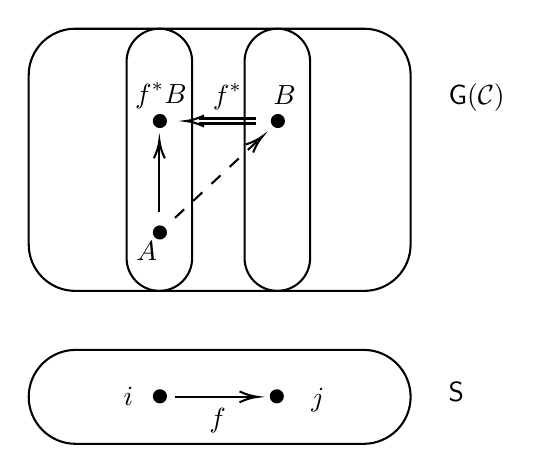
\begin{tikzpicture}[x=0.6pt,y=0.6pt,yscale=-1,xscale=1]
				%uncomment if require: \path (0,300); %set diagram left start at 0, and has height of 300
				
				%Rounded Rect [id:dp7645727072634361] 
				\draw   (60,57.96) .. controls (60,42.52) and (72.52,30) .. (87.96,30) -- (262.04,30) .. controls (277.48,30) and (290,42.52) .. (290,57.96) -- (290,159.93) .. controls (290,175.38) and (277.48,187.89) .. (262.04,187.89) -- (87.96,187.89) .. controls (72.52,187.89) and (60,175.38) .. (60,159.93) -- cycle ;
				%Rounded Rect [id:dp04913454848840337] 
				\draw   (60,251.71) .. controls (60,236.09) and (72.67,223.42) .. (88.29,223.42) -- (261.71,223.42) .. controls (277.33,223.42) and (290,236.09) .. (290,251.71) -- (290,251.71) .. controls (290,267.33) and (277.33,280) .. (261.71,280) -- (88.29,280) .. controls (72.67,280) and (60,267.33) .. (60,251.71) -- cycle ;
				%Shape: Ellipse [id:dp6766601997173525] 
				\draw  [fill={rgb, 255:red, 0; green, 0; blue, 0 }  ,fill opacity=1 ] (205.79,251.38) .. controls (205.79,249.38) and (207.41,247.76) .. (209.41,247.76) .. controls (211.41,247.76) and (213.03,249.38) .. (213.03,251.38) .. controls (213.03,253.38) and (211.41,255) .. (209.41,255) .. controls (207.41,255) and (205.79,253.38) .. (205.79,251.38) -- cycle ;
				%Straight Lines [id:da4121051063328982] 
				\draw    (147.89,251.71) -- (195.89,251.71) ;
				\draw [shift={(197.89,251.71)}, rotate = 180] [color={rgb, 255:red, 0; green, 0; blue, 0 }  ][line width=0.75]    (10.93,-3.29) .. controls (6.95,-1.4) and (3.31,-0.3) .. (0,0) .. controls (3.31,0.3) and (6.95,1.4) .. (10.93,3.29)   ;
				%Rounded Rect [id:dp07729214311167198] 
				\draw   (138.68,30) .. controls (149.58,30) and (158.42,38.84) .. (158.42,49.74) -- (158.42,168.16) .. controls (158.42,179.06) and (149.58,187.89) .. (138.68,187.89) -- (138.68,187.89) .. controls (127.78,187.89) and (118.95,179.06) .. (118.95,168.16) -- (118.95,49.74) .. controls (118.95,38.84) and (127.78,30) .. (138.68,30) -- cycle ;
				%Shape: Ellipse [id:dp389633265007308] 
				\draw  [fill={rgb, 255:red, 0; green, 0; blue, 0 }  ,fill opacity=1 ] (135.39,251.38) .. controls (135.39,249.38) and (137.01,247.76) .. (139.01,247.76) .. controls (141.01,247.76) and (142.63,249.38) .. (142.63,251.38) .. controls (142.63,253.38) and (141.01,255) .. (139.01,255) .. controls (137.01,255) and (135.39,253.38) .. (135.39,251.38) -- cycle ;
				%Rounded Rect [id:dp15413565880932678] 
				\draw   (209.74,30) .. controls (220.64,30) and (229.47,38.84) .. (229.47,49.74) -- (229.47,168.16) .. controls (229.47,179.06) and (220.64,187.89) .. (209.74,187.89) -- (209.74,187.89) .. controls (198.84,187.89) and (190,179.06) .. (190,168.16) -- (190,49.74) .. controls (190,38.84) and (198.84,30) .. (209.74,30) -- cycle ;
				%Shape: Ellipse [id:dp15402457161842187] 
				\draw  [fill={rgb, 255:red, 0; green, 0; blue, 0 }  ,fill opacity=1 ] (135.39,85.59) .. controls (135.39,83.59) and (137.01,81.97) .. (139.01,81.97) .. controls (141.01,81.97) and (142.63,83.59) .. (142.63,85.59) .. controls (142.63,87.59) and (141.01,89.21) .. (139.01,89.21) .. controls (137.01,89.21) and (135.39,87.59) .. (135.39,85.59) -- cycle ;
				%Shape: Ellipse [id:dp4979251025439946] 
				\draw  [fill={rgb, 255:red, 0; green, 0; blue, 0 }  ,fill opacity=1 ] (206.45,85.59) .. controls (206.45,83.59) and (208.07,81.97) .. (210.07,81.97) .. controls (212.06,81.97) and (213.68,83.59) .. (213.68,85.59) .. controls (213.68,87.59) and (212.06,89.21) .. (210.07,89.21) .. controls (208.07,89.21) and (206.45,87.59) .. (206.45,85.59) -- cycle ;
				%Shape: Ellipse [id:dp9026796796050416] 
				\draw  [fill={rgb, 255:red, 0; green, 0; blue, 0 }  ,fill opacity=1 ] (135.39,152.7) .. controls (135.39,150.7) and (137.01,149.08) .. (139.01,149.08) .. controls (141.01,149.08) and (142.63,150.7) .. (142.63,152.7) .. controls (142.63,154.7) and (141.01,156.32) .. (139.01,156.32) .. controls (137.01,156.32) and (135.39,154.7) .. (135.39,152.7) -- cycle ;
				%Straight Lines [id:da2600694132285619] 
				\draw    (138.68,140.53) -- (138.68,99.11) ;
				\draw [shift={(138.68,97.11)}, rotate = 90] [color={rgb, 255:red, 0; green, 0; blue, 0 }  ][line width=0.75]    (10.93,-3.29) .. controls (6.95,-1.4) and (3.31,-0.3) .. (0,0) .. controls (3.31,0.3) and (6.95,1.4) .. (10.93,3.29)   ;
				%Straight Lines [id:da9777401765397118] 
				\draw    (196.68,87.09) -- (162.63,87.09)(196.68,84.09) -- (162.63,84.09) ;
				\draw [shift={(154.63,85.59)}, rotate = 360] [color={rgb, 255:red, 0; green, 0; blue, 0 }  ][line width=0.75]    (10.93,-3.29) .. controls (6.95,-1.4) and (3.31,-0.3) .. (0,0) .. controls (3.31,0.3) and (6.95,1.4) .. (10.93,3.29)   ;
				%Straight Lines [id:da8835007806054442] 
				\draw  [dash pattern={on 4.5pt off 4.5pt}]  (148.11,143.9) -- (199.45,96.06) ;
				\draw [shift={(200.91,94.7)}, rotate = 137.02] [color={rgb, 255:red, 0; green, 0; blue, 0 }  ][line width=0.75]    (10.93,-3.29) .. controls (6.95,-1.4) and (3.31,-0.3) .. (0,0) .. controls (3.31,0.3) and (6.95,1.4) .. (10.93,3.29)   ;
				
				% Text Node
				\draw (311,241) node [anchor=north west][inner sep=0.75pt]   [align=left] {$\displaystyle \mathsf{S}$};
				% Text Node
				\draw (311,61) node [anchor=north west][inner sep=0.75pt]   [align=left] {$\displaystyle \mathsf{G}(\mathcal{C})$};
				% Text Node
				\draw (115.26,244.2) node [anchor=north west][inner sep=0.75pt]   [align=left] {$\displaystyle i$};
				% Text Node
				\draw (228.42,244.86) node [anchor=north west][inner sep=0.75pt]   [align=left] {$\displaystyle j$};
				% Text Node
				\draw (123,156.6) node [anchor=north west][inner sep=0.75pt]   [align=left] {$\displaystyle A$};
				% Text Node
				\draw (122.2,60.6) node [anchor=north west][inner sep=0.75pt]   [align=left] {$\displaystyle f^{*} B$};
				% Text Node
				\draw (205.4,62.2) node [anchor=north west][inner sep=0.75pt]   [align=left] {$\displaystyle B$};
				% Text Node
				\draw (167,256.6) node [anchor=north west][inner sep=0.75pt]   [align=left] {$\displaystyle f$};
				% Text Node
				\draw (169,61.4) node [anchor=north west][inner sep=0.75pt]   [align=left] {$\displaystyle f^{*}$};
				
			\end{tikzpicture}
		\end{center}
	\end{minipage}
	$$\big(gf,A\overset{\varphi}{\to}f^*B\overset{f^*(\psi)}{\to} f^*g^* C\overset{\gamma^{-1}}{\to} (gf)^* C\big)\colon (i,A)\to (k,C).$$
	$\gamma$ 的融贯性保证了上述复合的结合律, 使得 $\mathsf G(\mathcal C)$ 构成一个 $1$-范畴.
	$\mathsf G(\mathcal C)$ 到 $\mathcal S$ 有明显的投影函子 $(i,A)\mapsto i$, 这是一个纤维范畴. 将索引范畴对应到此纤维范畴的过程称为 \emph{Grothendieck 构造}, 它是一个 $2$-函子
	\[
	\mathsf G \colon \mathcal Cat_{\mathcal S} \to \mathcal Cat/\mathcal S.
	\]
\end{definition}

\begin{example}
	{(俯范畴作为索引范畴)}
	设范畴 $\mathcal C$ 有拉回, 即对态射 $f\colon c_1\to c_2$ 有俯范畴之间的函子 $f^*\colon \mathcal C/c_2 \to \mathcal C/c_1$. 进一步, 有 $2$-函子 $\mathcal C^{\op}\to\mathcal Cat$, 将对象 $c$ 对应到俯范畴 $\mathcal C/c$.
	其 Grothendieck 范畴为 $\mathcal C^{\bullet\to\bullet}$, 即 $\mathcal C$ 中的态射构成的范畴, 见例 \ref{over-category-fibration}.
\end{example}

Grothendieck 范畴的直观是 ``纤维丛的全空间''. 在一个 Grothendieck 范畴 $\mathsf G(\mathcal C)$ 中, 与 (带联络的) 纤维丛相似地, 我们可以定义\emph{垂直}和\emph{水平}的态射: 态射 $(\operatorname{id}_i,\varphi)$ 是垂直的 (即 ``纤维方向'' 的), 而 $(f,\operatorname{id}_A)$ 是水平的.
很明显, 任何态射 $(f,\varphi)\colon (i,A) \to (j,B)$ 都可分解为一个垂直态射
$(\operatorname{id}_i,\varphi)$
后接一个水平态射 $(f,\operatorname{id}_{f^*B})$.

在几何学中, 一个纤维丛的联络等同于在全空间上对每个点指定一些水平方向. 有了联络, 就可在纤维之间作平行移动. 要在范畴之间做类似的事情, 就需要将水平态射的概念抽象到一般的 ``纤维范畴'' $\pi\colon \mathcal C\to\mathcal S$, 而这将解释纤维范畴定义的动机.

\begin{definition}
	[label={prone-morphism}]
	{(水平态射)}
	设 $\mathcal C,\mathcal S$ 为 $1$-范畴, $\pi\colon \mathcal C\to\mathcal S$ 为函子.
	对于态射 $h\colon c'\to c$, 若以下条件成立, 则称之为 $\pi$-\emph{水平态射} (prone morphism, 又称 Cartesian morphism):
	对任意态射 $k\colon c''\to c$ 以及任意分解 $\pi(k) = \pi(h)x$, 存在唯一的态射 $\ell\colon c''\to c$ 满足 $k=h\ell$ 且 $x=\pi(\ell)$.
	% https://q.uiver.app/#q=WzAsNixbMSwyLCJcXHBpKGMnKSJdLFsyLDIsIlxccGkoYykiXSxbMCwzLCJcXGJ1bGxldCJdLFsxLDAsImMnIl0sWzAsMSwiYycnIl0sWzIsMCwiYyJdLFswLDEsIlxccGkoaCkiXSxbMiwwLCJ4Il0sWzQsMywiXFxleGlzdHMgISBcXGVsbCIsMCx7InN0eWxlIjp7ImJvZHkiOnsibmFtZSI6ImRhc2hlZCJ9fX1dLFszLDUsImgiXSxbNCw1LCJrIiwyXSxbMywwLCIiLDIseyJzaG9ydGVuIjp7InNvdXJjZSI6NjAsInRhcmdldCI6MTB9LCJsZXZlbCI6Mn1dLFsyLDEsIlxccGkoaykiLDJdXQ==
	\[\begin{tikzcd}[ampersand replacement=\&]
		\& {c'} \& c \\
		{c''} \\
		\& {\pi(c')} \& {\pi(c)} \\
		\bullet
		\arrow["{\pi(h)}", from=3-2, to=3-3]
		\arrow["x", from=4-1, to=3-2]
		\arrow["{\exists ! \ell}", dashed, from=2-1, to=1-2]
		\arrow["h", from=1-2, to=1-3]
		\arrow["k"', from=2-1, to=1-3]
		\arrow[shorten <=19pt, shorten >=3pt, Rightarrow, from=1-2, to=3-2]
		\arrow["{\pi(k)}"', from=4-1, to=3-3]
	\end{tikzcd}\]
\end{definition}

$\pi$-水平态射的直观为 ``拉回''; 且在下例中它完全就是拉回.

\begin{example}
	{(向量丛范畴中的水平态射)}
	继续例 \ref{vector-bundle-fibration}, %函子 $\pi\colon \mathsf {VBun} \to \mathsf {Man}$ 将向量丛 $E\to M$ 对应到 $M$.
	考虑下图,%沿映射 $f^*\colon N\to M$ 拉回向量丛 $E\to M$.
	其中 $K\to L$, $E\to M$ 为向量丛.
	% https://q.uiver.app/#q=WzAsNixbMSwxLCJOIl0sWzIsMSwiTSJdLFsyLDAsIkUiXSxbMSwwLCJmXipFIl0sWzAsMiwiTCJdLFswLDEsIksiXSxbMCwxLCJmIiwyXSxbMywwXSxbMywyXSxbMiwxXSxbNSw0XSxbNCwxXSxbNSwyXSxbNCwwXSxbNSwzLCJcXGV4aXN0cyAhIiwwLHsic3R5bGUiOnsiYm9keSI6eyJuYW1lIjoiZGFzaGVkIn19fV1d
	\[\begin{tikzcd}[ampersand replacement=\&]
		\& {f^*E} \& E \\
		K \& N \& M \\
		L
		\arrow["f"', from=2-2, to=2-3]
		\arrow[from=1-2, to=2-2]
		\arrow[from=1-2, to=1-3]
		\arrow[from=1-3, to=2-3]
		\arrow[from=2-1, to=3-1]
		\arrow[from=3-1, to=2-3]
		\arrow[from=2-1, to=1-3]
		\arrow[from=3-1, to=2-2]
		\arrow["{\exists !}", dashed, from=2-1, to=1-2]
	\end{tikzcd}\]
	由拉回的泛性质, 存在唯一的向量丛态射 $K\to f^*E$ 使其交换.
	这说明向量丛的拉回构成 $\pi\colon \mathsf {VBun} \to \mathsf {Top}$ 的水平态射.
\end{example}

\begin{definition}
	[label={Grothendieck-and-Street-fibration}]
	{(纤维范畴, Grothendieck 纤维化, Street 纤维化)}
	对于函子 $\pi\colon \mathcal C\to \mathcal S$,
	若如下条件成立, 则称之为\emph{纤维范畴} (fibered category, 或称\emph{ Grothendieck 纤维化}):
	对 $\mathcal C$ 的任意对象 $c$ 以及 $\mathcal S$ 中任意态射 $f\colon s\to \pi(c)$,
	都存在 $\pi$-水平态射 $\widetilde f\colon c'\to c$ 使得 $\pi(\widetilde f)= f$.
	换言之, \emph{若一个态射 $f$ 的终点有提升, 则该态射有水平提升 $\widetilde f$}.
	
	若上面条件中的 $\pi(\widetilde f)= f$ 改为较弱的条件 $\pi(\widetilde f) \simeq f$ (在 $\mathcal S/\pi(c)$ 中), 则称之为 \emph{Street 纤维化}\footnotemark{}.
	
	若 $\pi^{\op}\colon \mathcal C^{\op} \to \mathcal S^{\op}$ 为纤维化, 则称 $\pi$ 为\emph{对偶纤维化} (opfibration). 既是纤维化又是对偶纤维化的函子称为\emph{双纤维化} (bifibration).
%	对偶纤维化 $\pi\colon \mathcal C\to \mathcal S$ 的条件可具体表述为:
%	对 $\mathcal C$ 的任意对象 $c$ 以及 $\mathcal S$ 中任意态射 $f\colon \pi(c)\to s$,
%	都存在态射 $\widetilde f\colon c\to c'$ 使得 $\pi(\widetilde f)= f$,
%	.
\end{definition}
\footnotetext{Ross Street, 澳大利亚范畴学家.}

\begin{remark}
	[label={fibration-vs-cloven-fibration}]
	{(水平提升的唯一性与分裂纤维化)}
	在纤维化的定义 (\ref{Grothendieck-and-Street-fibration}) 中,
	没有提到水平提升 $\widetilde f$ 是唯一的; 但由水平态射的定义, $f$ 的任意两个水平提升 $\widetilde f_1,\widetilde f_2$ 之间由唯一的同构相联系.
	% https://q.uiver.app/#q=WzAsNSxbMCwyLCJzIl0sWzIsMCwiYyJdLFswLDEsImMnIl0sWzIsMiwiXFxwaShjKVxcIVxcIVxcISJdLFswLDAsImMnJyJdLFswLDMsImYiLDJdLFsyLDEsIlxcd2lkZXRpbGRlIGZfMSIsMl0sWzQsMSwiXFx3aWRldGlsZGUgZl8yIl0sWzIsNCwiXFxleGlzdHMgISIsMCx7Im9mZnNldCI6LTIsInN0eWxlIjp7ImJvZHkiOnsibmFtZSI6ImRhc2hlZCJ9fX1dLFs0LDIsIlxcZXhpc3RzICEiLDAseyJvZmZzZXQiOi0yLCJzdHlsZSI6eyJib2R5Ijp7Im5hbWUiOiJkYXNoZWQifX19XSxbNyw1LCIiLDIseyJzaG9ydGVuIjp7InNvdXJjZSI6NDAsInRhcmdldCI6MzB9fV1d
	\[\begin{tikzcd}[ampersand replacement=\&,row sep=small]
		{c''} \&\& c \\
		{c'} \\
		s \&\& {\pi(c)\!\!\!}
		\arrow[""{name=0, anchor=center, inner sep=0}, "{\widetilde f_2}", from=1-1, to=1-3]
		\arrow["{\exists !}", shift left=2, dashed, from=1-1, to=2-1]
		\arrow["{\exists !}", shift left=2, dashed, from=2-1, to=1-1]
		\arrow["{\widetilde f_1}"', from=2-1, to=1-3]
		\arrow[""{name=1, anchor=center, inner sep=0}, "f"', from=3-1, to=3-3]
		\arrow[shorten <=17pt, shorten >=13pt, Rightarrow, from=0, to=1]
	\end{tikzcd}\]
	\emph{假设选择公理}, 那么我们可以给每个 $f$ 选择一个水平提升;
	这额外的信息称为纤维化的\emph{分裂} (cleavage). 带有分裂的纤维化称作\emph{分裂纤维化} (cloven fibration, 或 split fibration).
\end{remark}

\begin{example}
	{(预层作为纤维范畴)}
	范畴 $\mathcal C$ 上的预层 $X\colon \mathcal C^{\op}\to\mathsf {Set}$ 可视为索引范畴 (纤维范畴), 其纤维为离散范畴. 此时 Grothendieck 构造 (定义 \ref{Grothendieck-construction}) 退化为 ``元素的范畴'' (定义 \ref{slice-over-presheaf}).
\end{example}

%\begin{example}
%	{(模)}
%	
%\end{example}

\begin{propdef}
	[label={fibre-category-indexed}]
	{(由纤维范畴给出索引范畴)}
	给定纤维范畴 $\pi\colon \mathcal C\to\mathcal S$, 我们构造相应的 $2$-函子 $\mathcal S^{\op} \to\mathcal Cat$.
	\begin{itemize}
		\item $\mathcal S$ 的对象 $X$ 对应范畴 $\mathcal C_X :=\pi^{-1}(X)$.
		\item 对于 $\mathcal S$ 中的态射 $f\colon X\to Y$, 如下定义函子 $f^*\colon \mathcal C_Y\to\mathcal C_X$,
		\begin{itemize}
			\item 对于 $\mathcal C_Y$ 的对象 $E$, 由纤维范畴的定义, 存在 $f$ 的水平提升 $\widetilde f\colon E'\to E$, 令 $f^*(E)=E'$ (这一步或者需要选择公理, 或者需要 $\pi$ 的一个分裂, 见注 \ref{fibration-vs-cloven-fibration}),
			\item 对于 $\mathcal C_Y$ 中的态射 $\varphi\colon E_1\to E_2$, 由水平态射的定义 (\ref{prone-morphism}), 下图中存在唯一的 $\varphi'\colon f^*E_1\to f^*E_2$.
			% https://q.uiver.app/#q=WzAsOCxbMiwxLCJFXzEiXSxbMywwLCJFXzIiXSxbMywyLCJZIl0sWzAsMywiWCJdLFsxLDAsImZeKkVfMiJdLFswLDEsImZeKkVfMSJdLFsxLDIsIlgiXSxbMiwzLCJZIl0sWzAsMSwiXFx2YXJwaGkiLDJdLFs1LDBdLFs0LDFdLFs1LDQsIlxcZXhpc3RzICFcXHZhcnBoaSciLDAseyJzdHlsZSI6eyJib2R5Ijp7Im5hbWUiOiJkYXNoZWQifX19XSxbMyw2LCJcXG9wZXJhdG9ybmFtZXtpZH1fWCJdLFszLDcsImYiLDJdLFs2LDIsImYiXSxbNywyLCJcXG9wZXJhdG9ybmFtZXtpZH1fWSIsMl0sWzQsMCwiIiwxLHsic3R5bGUiOnsiYm9keSI6eyJuYW1lIjoibm9uZSJ9LCJoZWFkIjp7Im5hbWUiOiJub25lIn19fV0sWzYsNywiIiwxLHsic3R5bGUiOnsiYm9keSI6eyJuYW1lIjoibm9uZSJ9LCJoZWFkIjp7Im5hbWUiOiJub25lIn19fV0sWzE2LDE3LCIiLDEseyJzaG9ydGVuIjp7InNvdXJjZSI6NDAsInRhcmdldCI6NDB9fV1d
			\[\begin{tikzcd}[ampersand replacement=\&,column sep=tiny,row sep=small]
				\& {f^*E_2} \&\& {E_2} \\
				{f^*E_1} \&\& {E_1} \\
				\& X \&\& Y \\
				X \&\& Y
				\arrow[from=1-2, to=1-4]
				\arrow[""{name=0, anchor=center, inner sep=0}, draw=none, from=1-2, to=2-3]
				\arrow["{\exists !\varphi'}", dashed, from=2-1, to=1-2]
				\arrow[from=2-1, to=2-3]
				\arrow["\varphi"', from=2-3, to=1-4]
				\arrow["f", from=3-2, to=3-4]
				\arrow[""{name=1, anchor=center, inner sep=0}, draw=none, from=3-2, to=4-3]
				\arrow["{\operatorname{id}_X}", from=4-1, to=3-2]
				\arrow["f"', from=4-1, to=4-3]
				\arrow["{\operatorname{id}_Y}"', from=4-3, to=3-4]
				\arrow[shorten <=17pt, shorten >=17pt, Rightarrow, from=0, to=1]
			\end{tikzcd}\]
			定义 $f^*(\varphi)=\varphi'$. 唯一性保证了该构造确实定义了一个函子.
		\end{itemize}
		\item 对于 $\mathcal S$ 中的态射 $f\colon X\to Y$, $g\colon Y\to Z$, 下图中存在唯一的同构 $f^*g^*\simeq (gf)^*$.
		% https://q.uiver.app/#q=WzAsNyxbMSwwLCJnXipFIl0sWzAsMiwiWCJdLFswLDAsImZeKmdeKkUiXSxbMSwyLCJZIl0sWzIsMiwiWiJdLFsyLDAsIkUiXSxbMCwxLCIoZ2YpXipFIl0sWzIsMF0sWzEsMywiZiIsMl0sWzMsNCwiZyIsMl0sWzAsNV0sWzYsNV0sWzIsNiwiXFxleGlzdHMgISIsMCx7Im9mZnNldCI6LTIsInN0eWxlIjp7ImJvZHkiOnsibmFtZSI6ImRhc2hlZCJ9fX1dLFs2LDIsIlxcZXhpc3RzICEiLDAseyJvZmZzZXQiOi0yLCJzdHlsZSI6eyJib2R5Ijp7Im5hbWUiOiJkYXNoZWQifX19XSxbMCwzLCIiLDEseyJzaG9ydGVuIjp7InNvdXJjZSI6MzAsInRhcmdldCI6MzB9LCJsZXZlbCI6Mn1dXQ==
		\[\begin{tikzcd}[ampersand replacement=\&,sep=small]
			{f^*g^*E} \& {g^*E} \& E \\
			{(gf)^*E} \\
			X \& Y \& Z
			\arrow[from=1-1, to=1-2]
			\arrow["{\exists !}", shift left=2, dashed, from=1-1, to=2-1]
			\arrow[from=1-2, to=1-3]
			\arrow[shorten <=10pt, shorten >=10pt, Rightarrow, from=1-2, to=3-2]
			\arrow["{\exists !}", shift left=2, dashed, from=2-1, to=1-1]
			\arrow[from=2-1, to=1-3]
			\arrow["f"', from=3-1, to=3-2]
			\arrow["g"', from=3-2, to=3-3]
		\end{tikzcd}\]
	\end{itemize}
	由上述讨论, 以及 $\mathcal S$ 是局部离散 $2$-范畴, 容易验证 $2$-函子的定义 (\ref{2-functor}) 要求的融贯性.
\end{propdef}

\begin{prop}
	[label={bifibration-induced-adjunction}]
	{(双纤维化产生伴随)}
	设 $\pi\colon \mathcal C\to\mathcal S$ 为双纤维化, 则 $\mathcal S$ 中的态射 $f\colon X\to Y$ 产生一对伴随
	% https://q.uiver.app/#q=WzAsMixbMCwwLCJcXG1hdGhjYWwgQ19YIl0sWzEsMCwiXFxtYXRoY2FsIENfWSJdLFswLDEsImZfISIsMCx7Im9mZnNldCI6LTJ9XSxbMSwwLCJmXioiLDAseyJvZmZzZXQiOi0yfV0sWzIsMywiIiwwLHsibGV2ZWwiOjEsInN0eWxlIjp7Im5hbWUiOiJhZGp1bmN0aW9uIn19XV0=
	\[\begin{tikzcd}[ampersand replacement=\&]
		{\mathcal C_X} \& {\mathcal C_Y}
		\arrow[""{name=0, anchor=center, inner sep=0}, "{f_!}", shift left=2, from=1-1, to=1-2]
		\arrow[""{name=1, anchor=center, inner sep=0}, "{f^*}", shift left=2, from=1-2, to=1-1]
		\arrow["\dashv"{anchor=center, rotate=-90}, draw=none, from=0, to=1]
	\end{tikzcd}\]
	其中 $f^*$ 是定义 \ref{fibre-category-indexed} 中的 $f^*$, 而 $f_!$ 是纤维范畴 $\pi^{\op}\colon \mathcal C^{\op} \to \mathcal S^{\op}$ 的相应构造.
\end{prop}
\begin{proof}
	这是由于自然同构
	\[
	\operatorname{Hom}_{\mathcal C_Y}(f_!-,-)\simeq\operatorname{Hom}_{\mathcal C}(-,-)\simeq\operatorname{Hom}_{\mathcal C_X}(-,f^*-).
	\]
\end{proof}

\begin{prop}
	{}
	在命题 \ref{bifibration-induced-adjunction} 的对应下, 一对伴随等同于 $\{0\to 1\}$ 上的一个双纤维化.
\end{prop}
\begin{proof}
	设有伴随
	% https://q.uiver.app/#q=WzAsMixbMCwwLCJcXG1hdGhjYWwgQ18wIl0sWzEsMCwiXFxtYXRoY2FsIENfMSJdLFswLDEsIkciLDIseyJsYWJlbF9wb3NpdGlvbiI6NDAsIm9mZnNldCI6Mn1dLFsxLDAsIkYiLDIseyJvZmZzZXQiOjJ9XSxbMywyLCIiLDIseyJsZXZlbCI6MSwic3R5bGUiOnsibmFtZSI6ImFkanVuY3Rpb24ifX1dXQ==
	$\begin{tikzcd}[ampersand replacement=\&]
		{\mathcal C_0} \& {\mathcal C_1},
		\arrow[""{name=0, anchor=center, inner sep=0}, "G", shift left=2, from=1-1, to=1-2]
		\arrow[""{name=1, anchor=center, inner sep=0}, "H", shift left=2, from=1-2, to=1-1]
		\arrow["\dashv"{anchor=center, rotate=-90}, draw=none, from=0, to=1]
	\end{tikzcd}$
	考虑如下的范畴 $\mathcal C$,
	\begin{itemize}
		\item 其对象类为 $\operatorname{Ob}\mathcal C = \operatorname{Ob}\mathcal C_0 \sqcup \operatorname{Ob}\mathcal C_1$;
		\item 态射集为 $\operatorname{Hom}_{\mathcal C}(c,c')=\begin{cases}
			\operatorname{Hom}_{\mathcal C_i}(c,c')& c,c'\in\operatorname{Ob} \mathcal C_i\\
			\operatorname{Hom}_{\mathcal C_1}(Gc,c')\text{ 即 }\operatorname{Hom}_{\mathcal C_0}(c,Hc') & c\in\operatorname{Ob}\mathcal C_0,c'\in\operatorname{Ob}\mathcal C_1\\
			\varnothing & c\in\operatorname{Ob}\mathcal C_1,c'\in\operatorname{Ob}\mathcal C_0
		\end{cases}$.
	\end{itemize}
	定义函子 $\pi\colon \mathcal C \to \{0\to 1\}$,
	将 $\mathcal C_0$ 的对象映射到 $0$, $\mathcal C_1$ 的对象映射到 $1$,
	$\mathcal C_0$ 中的态射映射到 $\operatorname{id}_0$,
	$\mathcal C_1$ 中的态射映射到 $\operatorname{id}_1$,
	其余的态射映射到 $f\colon 0\to 1$.
	我们验证 $\pi$ 是双纤维化.
%	\begin{itemize}
%		\item 对于 $c\in\operatorname{Ob}\mathcal C_0$, 单位 $\eta_c\in\operatorname{Hom}_{\mathcal C_0}(c,HGc)$ 给出态射 $\widetilde \eta_c\in\operatorname{Hom}_{\mathcal C}(c,Gc)$.
%		对任意 $c'\in\operatorname{Ob}\mathcal C_1$ 以及 $k\in\operatorname{Hom}_{\mathcal C}(c,c')$,
%		$k$ 唯一地穿过 $\widetilde \eta_c$.
%		\item 对于 $c'\in\operatorname{Ob}\mathcal C_1$, 余单位 $\varepsilon_{c'}\in\operatorname{Hom}_{\mathcal C_1}(GHc',c')$ 给出态射 $\widetilde \varepsilon_{c'}\in\operatorname{Hom}_{\mathcal C}(Hc',c')$.
%		对任意 $c\in\operatorname{Ob}\mathcal C_0$ 以及 $k\in \operatorname{Hom}_{\mathcal C}(c,c')$,
%		$k$ 唯一地穿过 $\widetilde \varepsilon_{c'}$.
%	\end{itemize}
%	% https://q.uiver.app/#q=WzAsMTIsWzAsMywiMCJdLFsxLDMsIjEiXSxbMCwxLCJjIl0sWzEsMSwiR2MiXSxbMiwwLCJjJyJdLFsyLDIsIjEiXSxbMywzLCIwIl0sWzQsMiwiMCJdLFs1LDIsIjEiXSxbMywxLCJjIl0sWzUsMCwiYyciXSxbNCwwLCJIYyciXSxbMiwzLCJcXHdpZGV0aWxkZSBcXGV0YV9jIiwyXSxbMiw0XSxbMyw0LCJcXGV4aXN0cyAhIiwyLHsic3R5bGUiOnsiYm9keSI6eyJuYW1lIjoiZGFzaGVkIn19fV0sWzAsMV0sWzAsNV0sWzEsNV0sWzYsN10sWzcsOF0sWzYsOF0sWzksMTAsImsiLDJdLFsxMSwxMCwiXFx3aWRldGlsZGUgXFx2YXJlcHNpbG9uX3tjJ30iXSxbOSwxMSwiXFxleGlzdHMgISIsMCx7InN0eWxlIjp7ImJvZHkiOnsibmFtZSI6ImRhc2hlZCJ9fX1dLFszLDE2LCIiLDAseyJzaG9ydGVuIjp7InNvdXJjZSI6MjAsInRhcmdldCI6MjB9fV0sWzIxLDcsIiIsMix7InNob3J0ZW4iOnsic291cmNlIjoyMCwidGFyZ2V0IjoyMH19XV0=
%	\[\begin{tikzcd}[ampersand replacement=\&,row sep=small]
%		\&\& {c'} \&\& {Hc'} \& {c'} \\
%		c \& Gc \&\& c \\
%		\&\& 1 \&\& 0 \& 1 \\
%		0 \& 1 \&\& 0
%		\arrow["{\widetilde \varepsilon_{c'}}", from=1-5, to=1-6]
%		\arrow[from=2-1, to=1-3]
%		\arrow["{\widetilde \eta_c}"', from=2-1, to=2-2]
%		\arrow["{\exists !}"', dashed, from=2-2, to=1-3]
%		\arrow["{\exists !}", dashed, from=2-4, to=1-5]
%		\arrow[""{name=0, anchor=center, inner sep=0}, "k"', from=2-4, to=1-6]
%		\arrow[from=3-5, to=3-6]
%		\arrow[""{name=1, anchor=center, inner sep=0}, from=4-1, to=3-3]
%		\arrow[from=4-1, to=4-2]
%		\arrow[from=4-2, to=3-3]
%		\arrow[from=4-4, to=3-5]
%		\arrow[from=4-4, to=3-6]
%		\arrow[shorten <=5pt, shorten >=5pt, Rightarrow, from=2-2, to=1]
%		\arrow[shorten <=5pt, shorten >=5pt, Rightarrow, from=0, to=3-5]
%	\end{tikzcd}\]
	% https://q.uiver.app/#q=WzAsOCxbMCwzLCIwIl0sWzIsMywiMSJdLFswLDEsImMiXSxbMiwxLCJHYyJdLFszLDAsImMnIl0sWzMsMiwiMSJdLFsxLDAsIkhjJyJdLFsxLDIsIjAiXSxbMiwzLCJcXHdpZGV0aWxkZSBcXGV0YV9jIiwyXSxbMiw0XSxbMyw0LCJcXGV4aXN0cyAhIiwyLHsic3R5bGUiOnsiYm9keSI6eyJuYW1lIjoiZGFzaGVkIn19fV0sWzAsMV0sWzAsNV0sWzEsNV0sWzYsNCwiXFx3aWRldGlsZGUgXFx2YXJlcHNpbG9uX3tjJ30iXSxbMiw2LCJcXGV4aXN0cyAhIiwwLHsic3R5bGUiOnsiYm9keSI6eyJuYW1lIjoiZGFzaGVkIn19fV0sWzAsN10sWzcsNV0sWzksMTIsIiIsMCx7InNob3J0ZW4iOnsic291cmNlIjo0MCwidGFyZ2V0Ijo0MH19XV0=
	\[\begin{tikzcd}[ampersand replacement=\&]
		\& {Hc'} \&\& {c'} \\
		c \&\& Gc \\
		\& 0 \&\& 1 \\
		0 \&\& 1
		\arrow["{\widetilde \varepsilon_{c'}}", from=1-2, to=1-4]
		\arrow["{\exists !}", dashed, from=2-1, to=1-2]
		\arrow["k"{name=0}, from=2-1, to=1-4]
		\arrow["{\widetilde \eta_c}"', from=2-1, to=2-3]
		\arrow["{\exists !}"', dashed, from=2-3, to=1-4]
		\arrow[from=3-2, to=3-4]
		\arrow[from=4-1, to=3-2]
		\arrow[""{name=1}, from=4-1, to=3-4]
		\arrow[from=4-1, to=4-3]
		\arrow[from=4-3, to=3-4]
		\arrow[shorten <=27pt, shorten >=27pt, Rightarrow, from=0, to=1]
	\end{tikzcd}\]
	如图, 对任意 $c\in\operatorname{Ob}\mathcal C_0$, $c'\in\operatorname{Ob}\mathcal C_1$,
	\begin{itemize}
		\item $\operatorname{id}_{Gc}\in\operatorname{Hom}_{\mathcal C_1}(Gc,Gc)$ (即 $\eta_c\in\operatorname{Hom}_{\mathcal C_0}(c,HGc)$) 给出 $\widetilde \eta_c\in\operatorname{Hom}_{\mathcal C}(c,Gc)$;
		\item $\operatorname{id}_{Hc'}\in\operatorname{Hom}_{\mathcal C_0}(Hc',Hc')$ (即 $\varepsilon_{c'}\in\operatorname{Hom}_{\mathcal C_1}(GHc',c')$) 给出 $\widetilde \varepsilon_{c'}\in\operatorname{Hom}_{\mathcal C}(Hc',c')$.
	\end{itemize}
	任意态射 $k\in\operatorname{Hom}_{\mathcal C}(c,c')$ 唯一地穿过 $\widetilde \eta_c$ 与 $\widetilde \varepsilon_{c'}$. 这说明 $\widetilde \eta_c$ 为 $\pi^{\op}$-水平态射, 而 $\widetilde \varepsilon_{c'}$ 为 $\pi$-水平态射; 从而 $\pi,\pi^{\op}$ 均为纤维化. 很明显, 该双纤维化在命题 \ref{bifibration-induced-adjunction} 的对应下给出的伴随正是 $G\dashv H$.
\end{proof}

\begin{remark}
	{}
	事实上, 双纤维化 $\pi\colon \mathcal C\to \mathcal S$ 等同于 $2$-函子 $\mathcal S^{\op} \to \mathcal Cat_{\text{Adj}}$ ($\mathcal Cat_{\text{Adj}}$ 的定义见 \ref{cat-adj}).
\end{remark}

\begin{example}
	{(双纤维化产生的伴随的例子)}
	\begin{itemize}
		\item 例 \ref{mod-ring-fibration} 中的纤维化 $\mathsf {Mod}\to\mathsf {Ring}$ 是双纤维化. 环同态 $\varphi\colon A\to B$ 诱导了模范畴之间的伴随 $\varphi_!\dashv \varphi^*$, $\varphi_!=(-)\otimes_A B$, $\varphi^*=\operatorname{Hom}_B(B,-)$ (见例 \ref{change-of-rings}).
		\item 设范畴 $\mathcal C$ 具有拉回, 则例 \ref{over-category-fibration} 提到的函子 $t\colon \mathcal C^{\bullet\to\bullet}\to\mathcal C$ 是双纤维化. $\mathcal C$ 中的态射 $f\colon X\to Y$ 诱导了俯范畴之间的伴随 $\Sigma_f=f_! \dashv f^*$ (见例 \ref{sigma-adjoint}).
	\end{itemize}
\end{example}

\subsection{等变对象}



\section{下降}

\todo{}

% Grothendieck 1959 Descente par morphismes fid\'element plats

% Grothendieck 1971 Cat\'egories fibr\'ees et descente

% Joyal--Tierney 1984 Extension of the Galois theory of Grothendieck

粗略地说, \emph{下降} (descent) 是许多场合出现的一种现象: 在一族变化的范畴 (即纤维范畴) $\mathcal C_X$ 中, 对于某种态射 $f\colon Y\to X$, 为了给出 $\mathcal C_X$ 中的一个对象 $u$, 只需要给出其 ``逆像'' $f^*(u)$ 以及某种额外的信息, 有时称为 ``粘贴资料'' (gluing datum) $\xi$. 称 $(f^*(u),\xi)$ 为一个\emph{下降资料} (descent datum, 复数 data). 当 $Y$ 是 $X$ 的某种覆盖时, 下降资料是层条件的类比, 下降的现象说明某些对象和态射可 ``局部地'' 定义.

\begin{example}
	{(向量丛的下降)}
	设拓扑空间 $X$ 有开覆盖 $\{U_i\}$; 令 $Y=\coprod_i U_i$, 所有 $U_i$ 的嵌入给出了映射 $p\colon Y\to X$.
	此时, 为了给出 $X$ 上的一个向量丛 $E$, 只需要给出 $Y$ 上的一个向量丛 $F$ ($F=p^*(E)$), 也即每个 $U_i$ 上的一个向量丛 $F_i$, 以及 $U_i, U_j$ 相交之处的粘贴资料
	\[
	\varphi_{ij}\colon F_i|_{U_i\cap U_j} \overset{\simeq}{\longrightarrow} F_j|_{U_i\cap U_j},
	\]
	满足 $\varphi_{ii}=\operatorname{id}_{F_i}$, 以及交换图
	% https://q.uiver.app/#q=WzAsMyxbMCwwLCJGX3tpfXxfe1VfaVxcY2FwIFVfalxcY2FwIFVfa30iXSxbMiwwLCJGX2t8X3tVX2lcXGNhcCBVX2pcXGNhcCBVX2t9Il0sWzEsMSwiRl9qfF97VV9pXFxjYXAgVV9qXFxjYXAgVV9rfSJdLFswLDEsIlxcdmFycGhpX3tpa30iXSxbMCwyLCJcXHZhcnBoaV97aWp9IiwyXSxbMiwxLCJcXHZhcnBoaV97amt9IiwyXV0=
	\[\begin{tikzcd}[ampersand replacement=\&]
		{F_{i}|_{U_i\cap U_j\cap U_k}} \&\& {F_k|_{U_i\cap U_j\cap U_k}.} \\
		\& {F_j|_{U_i\cap U_j\cap U_k}.}
		\arrow["{\varphi_{ik}}", from=1-1, to=1-3]
		\arrow["{\varphi_{ij}}"', from=1-1, to=2-2]
		\arrow["{\varphi_{jk}}"', from=2-2, to=1-3]
	\end{tikzcd}\]
	
	上述粘贴资料可表示为更抽象的形式.
	注意到
	\begin{equation}
		Y\times_X Y\simeq\coprod_{i,j} U_i\cap U_j,\quad Y\times_X Y\times_X Y\simeq\coprod_{i,j,k} U_i\cap U_j\cap U_k,
		\tag{$\star$}
	\end{equation}
	记 $\pi_\alpha\colon Y\times_X Y \to Y$ 为第 $\alpha$ 分量的投影 ($\alpha = 1,2$), $\pi_{\alpha \beta}\colon Y\times_X Y\times_X Y\to Y\times_X Y$ 为第 $\alpha ,\beta$ 分量的投影 ($1\leq \alpha <\beta \leq 3$),
	$\Delta\colon Y\to Y\times_X Y$ 为对角映射;
	这些映射满足如下的关系:
	$$\pi_1\pi_{13}=\pi_1\pi_{12}, \quad \pi_1\pi_{23}=\pi_2\pi_{12}, \quad \pi_2\pi_{13}=\pi_2\pi_{23},\quad
	\pi_1\Delta = \pi_2\Delta = \operatorname{id}_Y.$$
	在 $(\star)$ 的观点下, 这些映射可分别写为
	$$\Delta = (U_i \to U_i\cap U_i)_i,\ \pi_1 = \big(U_i\cap U_j\hookrightarrow U_i\big)_{i,j},\ \pi_{12} = \big( U_i\cap U_j\cap U_k \hookrightarrow U_i \cap U_j\big)_{i,j,k}.$$
	%而 $F|_{U_i\cap U_j}$
	故对于 $F=(F_i)_i$, 有 $\pi_1^*F = (F_i|_{U_i\cap U_j})_{i,j}$, $\pi_2^*F = (F_j|_{U_i\cap U_j})_{i,j}$, $\pi_{13}^*\pi_1^*F =\pi_{12}^*\pi_1^*F = (F_i|_{U_i\cap U_j\cap U_k})_{i,j,k}$ 等等.
	那么粘贴资料等同于 $Y\times_X Y$ 上的向量丛同构
	\[
	\varphi\colon \pi_1^*F \overset{\simeq}{\longrightarrow} \pi_2^*F,
	\]
	%注意到因为 $F\times_X Y \simeq \coprod_{i,j}F_i|_{U_i\cap U_j}$,
	%$Y\times_X F \simeq \coprod_{i,j}F_j|_{U_i\cap U_j}$, 上述粘贴资料也等同于一个 $Y\times_X Y$ 上的向量丛的同构
	满足 $\Delta^*\varphi = \operatorname{id}_{F}$ 以及交换图
	% https://q.uiver.app/#q=WzAsNixbMSwwLCJcXHBpX3sxM31eKlxccGlfMV4qRiJdLFs0LDAsIlxccGlfezEzfV4qXFxwaV8yXipGIl0sWzIsMywiXFxwaV97MTJ9XipcXHBpXzJeKkYiXSxbMCwxLCJcXHBpX3sxMn1eKlxccGlfMV4qRiJdLFs1LDEsIlxccGlfezIzfV4qXFxwaV8yXiogRiJdLFszLDMsIlxccGlfezIzfV4qXFxwaV8xXiogRiJdLFswLDEsIlxccGlfezEzfV4qKFxcdmFycGhpKSJdLFszLDIsIlxccGlfezEyfV4qKFxcdmFycGhpKSIsMl0sWzUsNCwiXFxwaV97MjN9XiooXFx2YXJwaGkpIiwyXSxbMiw1LCIiLDIseyJsZXZlbCI6Miwic3R5bGUiOnsiaGVhZCI6eyJuYW1lIjoibm9uZSJ9fX1dLFswLDMsIiIsMix7ImxldmVsIjoyLCJzdHlsZSI6eyJoZWFkIjp7Im5hbWUiOiJub25lIn19fV0sWzEsNCwiIiwwLHsibGV2ZWwiOjIsInN0eWxlIjp7ImhlYWQiOnsibmFtZSI6Im5vbmUifX19XV0=
	\[\begin{tikzcd}[ampersand replacement=\&,sep=tiny]
		\& {\pi_{13}^*\pi_1^*F} \&\&\& {\pi_{13}^*\pi_2^*F} \\
		{\pi_{12}^*\pi_1^*F} \&\&\&\&\& {\pi_{23}^*\pi_2^* F.} \\
		\\
		\&\& {\pi_{12}^*\pi_2^*F} \& {\pi_{23}^*\pi_1^* F}
		\arrow["{\pi_{13}^*(\varphi)}", from=1-2, to=1-5]
		\arrow[Rightarrow, no head, from=1-2, to=2-1]
		\arrow[Rightarrow, no head, from=1-5, to=2-6]
		\arrow["{\pi_{12}^*(\varphi)}"', from=2-1, to=4-3]
		\arrow[Rightarrow, no head, from=4-3, to=4-4]
		\arrow["{\pi_{23}^*(\varphi)}"', from=4-4, to=2-6]
	\end{tikzcd}\]
	%也即 (注意到 $F\times_X Y \simeq \coprod_{i,j}F_i|_{U_i\cap U_j}$, $Y\times_X F \simeq \coprod_{i,j}F_j|_{U_i\cap U_j}$)
	%\[
%	$\varphi\colon F\times_X Y \to Y\times_X F$,
%	% https://q.uiver.app/#q=WzAsMyxbMCwwLCJGXFx0aW1lc19YIFlcXHRpbWVzX1ggWSJdLFsxLDEsIllcXHRpbWVzX1ggRiBcXHRpbWVzX1ggWSJdLFsyLDAsIllcXHRpbWVzX1ggWSBcXHRpbWVzX1ggRiJdLFswLDEsIjAsMSIsMl0sWzEsMiwiMSwyIiwyXSxbMCwyLCIwLDIiXV0=
%	\[\begin{tikzcd}[ampersand replacement=\&]
%		{F\times_X Y\times_X Y} \&\& {Y\times_X Y \times_X F,} \\
%		\& {Y\times_X F \times_X Y}
%		\arrow["{1,3}", from=1-1, to=1-3]
%		\arrow["{1,2}"', from=1-1, to=2-2]
%		\arrow["{2,3}"', from=2-2, to=1-3]
%	\end{tikzcd}\]
	
%	粘贴资料尚有另一种表示方式. 注意到下图的右边小方块以及大长方块为拉回,
%	% https://q.uiver.app/#q=WzAsNixbMCwwLCJGXFx0aW1lc19YIFkiXSxbMSwwLCJZXFx0aW1lc19YIFkiXSxbMiwwLCJZIl0sWzEsMSwiWSJdLFswLDEsIkYiXSxbMiwxLCJYIl0sWzAsNF0sWzQsM10sWzMsNV0sWzAsMV0sWzEsMiwiXFxwaV8yIl0sWzIsNV0sWzEsMywiXFxwaV8xIiwyXV0=
%	\[\begin{tikzcd}[ampersand replacement=\&]
%		{F\times_X Y} \& {Y\times_X Y} \& Y \\
%		F \& Y \& X
%		\arrow[from=1-1, to=1-2]
%		\arrow[from=1-1, to=2-1]
%		\arrow["{\pi_2}", from=1-2, to=1-3]
%		\arrow["{\pi_1}"', from=1-2, to=2-2]
%		\arrow[from=1-3, to=2-3]
%		\arrow[from=2-1, to=2-2]
%		\arrow[from=2-2, to=2-3]
%	\end{tikzcd}\]
	注意到 $\pi_1^*F = F\times_Y(Y\times_X Y)\simeq F\times_X Y$, 类似地 $\pi_2^*F\simeq Y\times_X F$, $\pi_{13}^*\pi_1^*F \simeq F\times_X Y \times_X Y$ 等等; 故粘贴资料也可表示为一个同构 $\varphi\colon F\times_X Y\to Y\times_X F$,
	满足交换图
	\[\begin{tikzcd}[ampersand replacement=\&]
		{F\times_X Y\times_X Y} \&\& {Y\times_X Y \times_X F.} \\
		\& {Y\times_X F \times_X Y}
		\arrow["{\pi_{13}^*(\varphi)}", from=1-1, to=1-3]
		\arrow["{\pi_{12}^*(\varphi)}"', from=1-1, to=2-2]
		\arrow["{\pi_{23}^*(\varphi)}"', from=2-2, to=1-3]
	\end{tikzcd}\]
\end{example}

\begin{example}
	{(模的下降)}
	设环 $R$ 的谱 $\operatorname{Spec}(R)$ 有一个\emph{有限的}开覆盖 $\{\operatorname{Spec}R_{f_i}\}_{1\leq i\leq n}$, 其中 $f_i\in R$ 生成了 $R$ 的单位理想. (关于谱的开覆盖, 见例 \ref{open-sublocale-of-spectrum}.)
	令 $S=\prod_{i=1}^n R_{f_i}$, 一个 $S$-模 $M$ 等同于一组 $R_{f_i}$-模 $M_i$. 此时, 为了给出一个 $R$-模, 只需要给出一个 $S$ 模 $M$, 以及 $R_{f_if_j}$ 上的粘贴资料
	\[
		\varphi_{ij}\colon (M_i)_{f_j} \overset{\simeq}{\longrightarrow} (M_j)_{f_i}, %\varphi_{jk}\varphi_{ij}=\varphi_{ik}.
	\]
	满足 $\varphi_{ii} = \operatorname{id}_{M_i}$, 以及交换图
	% https://q.uiver.app/#q=WzAsMyxbMCwwLCIoTV9pKV97Zl9qZl9rfSJdLFsyLDAsIihNX2spX3tmX2lmX2p9Il0sWzEsMSwiKE1failfe2ZfaWZfa30iXSxbMCwxLCJcXHZhcnBoaV97aWt9Il0sWzAsMiwiXFx2YXJwaGlfe2lqfSIsMl0sWzIsMSwiXFx2YXJwaGlfe2prfSIsMl1d
	\[\begin{tikzcd}[ampersand replacement=\&]
		{(M_i)_{f_jf_k}} \&\& {(M_k)_{f_if_j}} \\
		\& {(M_j)_{f_if_k}.}
		\arrow["{\varphi_{ik}}", from=1-1, to=1-3]
		\arrow["{\varphi_{ij}}"', from=1-1, to=2-2]
		\arrow["{\varphi_{jk}}"', from=2-2, to=1-3]
	\end{tikzcd}\]
	%在代数中, 模的局部化
	(注. $(M_i)_{f_j}$ 是 $M_i$ 关于 $f_j$ 生成的乘法封闭子集 $\{1,f_j,f_j^2,\cdots\}$ 的局部化, 见例 \ref{localization-module}. 这个局部化对应到开子空间 $\operatorname{Spec}R_{f_i}$ 的限制. 对任意两个元素 $f_i,f_j$, 作为 $\operatorname{Spec}R$ 的子空间有 $\operatorname{Spec}R_{f_i}\cap\operatorname{Spec}R_{f_j} = \operatorname{Spec}(R_{f_i}\otimes_R R_{f_j})= \operatorname{Spec}R_{f_if_j}$.)
	
	上述粘贴资料可表示为更抽象的形式.
	注意到
	\begin{equation}
		S\otimes_R S \simeq \prod_{i,j=1}^n R_{f_i}\otimes_R R_{f_j} \simeq \prod_{i,j=1}^n R_{f_if_j},\quad
		S\otimes_R S \otimes_R S \simeq \prod_{i,j,k=1}^n R_{f_if_jf_k},
		\tag{$\star\star$}
	\end{equation}
	记 $\mu_\alpha \colon S \to S\otimes_R S$ 为第 $\alpha$ 分量的含入 ($\alpha =1,2$),
	$\mu_{\alpha \beta}\colon S\otimes_R S \to S\otimes_R S\otimes_R S$ 为第 $\alpha ,\beta$ 分量的含入 ($1\leq \alpha <\beta \leq 3$),
	$m\colon S\otimes_R S \to S$ 为乘法映射, 这些映射满足如下的关系:
	\[
	\mu_{12}\mu_1 = \mu_{13}\mu_1,\quad \mu_{12}\mu_2 = \mu_{23}\mu_1,\quad
	\mu_{23}\mu_2 = \mu_{13}\mu_2,\quad
	m\mu_1 = m\mu_2 = \operatorname{id}_S.
	\]
	在 $(\star\star)$ 的观点下, %这些映射可分别写为\todo{}
	\[
	m\colon (a_{ij})_{1\leq i,j\leq n}\mapsto (a_{ii})_{1\leq i\leq n},
	\ 
	\mu_1 \colon (a_i)_{1\leq i\leq n}\mapsto (a_{i})_{1\leq i,j\leq n}.
	\]
	
	对于环同态 $f\colon A\to B$, 考虑函子 $f_!={(-)\otimes_A B}\colon A\mathsf {Mod} \to B\mathsf {Mod}$.
	故对于 $M=(M_i)_i$, 有 $(\mu_1)_! M \simeq M\otimes_{S}(S\otimes_R S) \simeq M\otimes_R S = \big((M_i)_{f_j}\big)_{i,j}$, % \todo{错误} (注意 $R$-模范畴中, 下图的右边方块以及大长方块为推出).
	$(\mu_{13})_!(\mu_1)_! M=(\mu_{12})_!(\mu_1)_! M = \big((M_i)_{f_jf_k}\big)_{i,j,k}$ 等等.
%	% https://q.uiver.app/#q=WzAsNixbMiwxLCJSIl0sWzIsMCwiUyJdLFsxLDEsIlMiXSxbMSwwLCJTXFxvdGltZXNfUiBTIl0sWzAsMSwiTSJdLFswLDAsIk1cXG90aW1lc19SIFMiXSxbMiwzLCJcXG11XzEiXSxbMSwzLCJcXG11XzIiLDJdLFswLDJdLFswLDFdLFsyLDRdLFs0LDVdLFszLDVdXQ==
%	\[\begin{tikzcd}[ampersand replacement=\&]
%		{M\otimes_R S} \& {S\otimes_R S} \& S \\
%		M \& S \& R
%		\arrow[from=1-2, to=1-1]
%		\arrow["{\mu_2}"', from=1-3, to=1-2]
%		\arrow[from=2-1, to=1-1]
%		\arrow["{\mu_1}", from=2-2, to=1-2]
%		\arrow[from=2-2, to=2-1]
%		\arrow[from=2-3, to=1-3]
%		\arrow[from=2-3, to=2-2]
%	\end{tikzcd}\]
	那么粘贴资料等同于 $S\otimes_R S$ 上的模同构
	\[
	\varphi\colon (\mu_1)_! M \overset{\simeq}{\longrightarrow} (\mu_2)_! M,
	\]
	%注意到因为 $F\times_X Y \simeq \coprod_{i,j}F_i|_{U_i\cap U_j}$,
	%$Y\times_X F \simeq \coprod_{i,j}F_j|_{U_i\cap U_j}$, 上述粘贴资料也等同于一个 $Y\times_X Y$ 上的向量丛的同构
	满足 $m_!\varphi = \operatorname{id}_{M}$ 以及交换图
	% https://q.uiver.app/#q=WzAsNixbMSwwLCIoXFxtdV97MTN9KV8hKFxcbXVfMSlfIUZcXGhzcGFjZXstMmVtfSJdLFs0LDAsIlxcaHNwYWNley0yZW19KFxcbXVfezEzfSlfIShcXG11XzIpXyFGIl0sWzIsMywiKFxcbXVfezEyfSlfIShcXG11XzIpXyFGIl0sWzAsMSwiKFxcbXVfezEyfSlfIShcXG11XzEpXyFGIl0sWzUsMSwiKFxcbXVfezIzfSlfIShcXG11XzIpXyFGLiJdLFszLDMsIihcXG11X3syM30pXyEoXFxtdV8xKV8hRiJdLFswLDEsIihcXG11X3sxM30pXyEoXFx2YXJwaGkpIiwwLHsic2hvcnRlbiI6eyJzb3VyY2UiOjIwLCJ0YXJnZXQiOjIwfX1dLFszLDIsIihcXG11X3sxMn0pXyEoXFx2YXJwaGkpIiwyXSxbNSw0LCIoXFxtdV97MjN9KV8hKFxcdmFycGhpKSIsMl0sWzIsNSwiIiwyLHsibGV2ZWwiOjIsInN0eWxlIjp7ImhlYWQiOnsibmFtZSI6Im5vbmUifX19XSxbMCwzLCIiLDIseyJsZXZlbCI6Miwic3R5bGUiOnsiaGVhZCI6eyJuYW1lIjoibm9uZSJ9fX1dLFsxLDQsIiIsMCx7ImxldmVsIjoyLCJzdHlsZSI6eyJoZWFkIjp7Im5hbWUiOiJub25lIn19fV1d
	\[\begin{tikzcd}[ampersand replacement=\&,sep=tiny]
		\& {(\mu_{13})_!(\mu_1)_!M\hspace{-3em}} \&\&\& {\hspace{-3em}(\mu_{13})_!(\mu_2)_!M} \\
		{(\mu_{12})_!(\mu_1)_!M} \&\&\&\&\& {(\mu_{23})_!(\mu_2)_!M.} \\
		\\
		\&\& {(\mu_{12})_!(\mu_2)_!M} \& {(\mu_{23})_!(\mu_1)_!M}
		\arrow["{(\mu_{13})_!(\varphi)}", shorten <=32pt, shorten >=32pt, from=1-2, to=1-5]
		\arrow[Rightarrow, no head, from=1-2, to=2-1]
		\arrow[Rightarrow, no head, from=1-5, to=2-6]
		\arrow["{(\mu_{12})_!(\varphi)}"', from=2-1, to=4-3]
		\arrow[Rightarrow, no head, from=4-3, to=4-4]
		\arrow["{(\mu_{23})_!(\varphi)}"', from=4-4, to=2-6]
	\end{tikzcd}\]
	也即一个 $S\otimes_R S$-模同构
	\[
		\varphi\colon M\otimes_{R}S \to S\otimes_R M,
	\]
	满足
	% https://q.uiver.app/#q=WzAsMyxbMCwwLCJNXFxvdGltZXNfUiBTIFxcb3RpbWVzX1IgUyJdLFsyLDAsIlNcXG90aW1lc19SIFMgXFxvdGltZXNfUiBNIl0sWzEsMSwiU1xcb3RpbWVzX1IgTSBcXG90aW1lc19SIFMiXSxbMCwxLCIwLDIiXSxbMCwyLCIwLDEiLDJdLFsyLDEsIjEsMiIsMl1d
	\[\begin{tikzcd}[ampersand replacement=\&]
			{M\otimes_R S \otimes_R S} \&\& {S\otimes_R S \otimes_R M.} \\
			\& {S\otimes_R M \otimes_R S}
			\arrow["{(\mu_{13})_!(\varphi)}", from=1-1, to=1-3]
			\arrow["{(\mu_{12})_!(\varphi)}"', from=1-1, to=2-2]
			\arrow["{(\mu_{23})_!(\varphi)}"', from=2-2, to=1-3]
		\end{tikzcd}\]
\end{example}

\begin{example}
	{(``丛'' 的下降)}
	% codomain bifibration
	
\end{example}

% Moerdijk Descent Theory for Toposes : 群胚作用

\begin{definition}
	{(用单子表达下降)}
	% monadic descent applied to codomain fibrations archetypically exhibits the nature of monadic descent
	设 $\pi\colon \mathcal C\to \mathcal S$ 为双纤维化. 对于 $\mathcal S$ 中的态射 $f\colon X\to Y$,
	% https://ncatlab.org/nlab/show/monadic+descent
	定义\emph{下降资料的范畴} $\operatorname{Des}_\pi(f)$ 为伴随 $f_!\dashv f^*$ 对应的单子 $f^*f_!$ 的代数范畴, 也即
	\begin{itemize}
		\item $\operatorname{Des}_\pi(f)$ 的对象为\todo{}
	\end{itemize}
\end{definition}

\section{内范畴}

\begin{definition}
	{(内范畴)}
	% Diaconescu, 
	设范畴 $\mathcal S$ 具有拉回 (实际上不需要存在全部的拉回, 只需要存在下面用到的拉回即可).
	定义 $\mathcal S$ 上的一个\emph{内范畴} (internal category) $C$ 为如下资料,
	\begin{itemize}
		\item 对象 $C_0,C_1$, 分别代表 ``对象集'' 与 ``态射集'';
		\item 态射 $s,t\colon C_1\to C_0$, 分别代表态射的起点与终点;
		\item 态射 $e\colon C_0\to C_1$, 代表对象上的恒等态射;
		\item 态射 $c\colon C_1\times_{C_0} C_1\to C_1$, 代表态射的复合;
	\end{itemize}
	满足如下条件,
	\begin{itemize}
		\item $se=te=\operatorname{id}_{C_0}$ (恒等态射的起点和终点是自己);
		\item $sc=s\pi_1, tc=t\pi_2$ (复合态射的起点和终点);
		\item $c(c\times\operatorname{id}_{C_1})=c(\operatorname{id}_{C_1}\times c)$ (结合律);
		\item $c(\operatorname{id}_{C_1}\times e)=\pi_1,c(e\times \operatorname{id}_{C_1})=\pi_2$ (单位律).
	\end{itemize}
	%\todo{两者为何等价?}
	% 似乎是因为 Cartesian theory, Elephant D1.3.4
	
	对于\topos{}或正则范畴, $\mathcal S$ 的内范畴也可直接定义为小范畴的理论在 $\mathcal S$ 中的模型 (例 \ref{small-category-language}, 例 \ref{small-category-theory}).
	
	对于内范畴 $C,D$, 定义一个\emph{内函子} (internal functor) $f\colon C\to D$ 为态射 $f_0\colon C_0\to D_0$, $f_1\colon C_1\to D_1$, 要求与所有结构态射 $s,t,e,c$ 相容. 对于内函子 $f,g\colon C\to D$, 定义\emph{内自然变换} (internal natural transformation) $\alpha\colon f\to g$ 为态射 $\alpha\colon C_0\to D_1$, 满足 $s\alpha = f_0$, $t\alpha = g_0$, 且 $c(\alpha t,f_1) = c(g_1,\alpha s)\colon C_1\to D_1$. 其中最后一个等式对应交换图
	% https://q.uiver.app/#q=WzAsNCxbMSwwLCJnKGMpIl0sWzEsMSwiZyhkKSJdLFswLDAsImYoYykiXSxbMCwxLCJmKGQpIl0sWzAsMSwiZyhoKSJdLFsyLDMsImYoaCkiLDJdLFsyLDAsIlxcYWxwaGFfYyJdLFszLDEsIlxcYWxwaGFfZCIsMl1d
	\[\begin{tikzcd}[ampersand replacement=\&]
		{f(c)} \& {g(c)} \\
		{f(d)} \& {g(d).}
		\arrow["{g(h)}", from=1-2, to=2-2]
		\arrow["{f(h)}"', from=1-1, to=2-1]
		\arrow["{\alpha_c}", from=1-1, to=1-2]
		\arrow["{\alpha_d}"', from=2-1, to=2-2]
	\end{tikzcd}\]
	$\mathcal S$ 上的内范畴, 内函子与内自然变换构成 $2$-范畴 $\mathcal Cat(\mathcal S)$.
\end{definition}

\begin{remark}
	{(内脉)}
	通过\emph{内脉} (internal nerve) 操作, $\mathcal S$ 上的内范畴 $C$ 可视为 $\mathcal S$ 中的单纯对象 $N(C)\colon \Delta^{\op}\to\mathcal S$, 其中 $$N(C)_n:= \underbrace{C_1\times_{C_0}C_1\times_{C_0}\cdots\times_{C_0} C_1}_{\text{$n$ 个 $C_1$}}$$ 是 ``$n$ 个首尾相连态射的集合''. 由此, $\mathcal S$ 上的内范畴等同于保持拉回的函子 $\Delta^{\op}\to \mathcal S$. 此时内范畴之间的内函子对应\emph{单纯同伦}.
\end{remark}

\begin{example}
	{(Lie 群, Lie 群胚)}
	回忆 Lie 群是光滑流形范畴 $\mathsf {Man}$ 中的群. 正如群胚是群的推广, 我们可定义 Lie 群胚为 $\mathsf {Man}$ 的内群胚. 读者可尝试写下\emph{内群胚}的定义, 即在内范畴的基础上增加一个态射 $i\colon C_1\to C_1$ 表示态射的逆, 满足 $si=t,ti=s,c(i,\operatorname{id})=et,c(\operatorname{id},i)=es$.
	那么, Lie 群则是 $\mathsf {Man}$ 中以一个点为 ``对象集'' 的内群胚.
\end{example}

\begin{definition}
	{(内范畴对应的索引范畴)}
	设 $C$ 是 $\mathcal S$ 上的内范畴. 定义索引范畴 $[C]\colon \mathcal S^{\op}\to \mathcal Cat$ 如下:
	\begin{itemize}
		\item 将 $\mathcal S$ 的对象 $I$ 对应到范畴 $C^I$, 其对象为态射 $I\to C_0$, 态射为态射 $I\to C_1$;
		\item 将 $\mathcal S$ 中的态射 $f\colon I\to J$ 对应到函子 $f^*\colon C^J\to C^I$.
	\end{itemize}
	这是 ``对象族范畴'' (例 \ref{category-of-set-indexed-families}) 的推广. 范畴 $C^I$ 中的对象是 ``以 $I$ 为索引的一族对象''.
\end{definition}

% 内函子范畴到底是什么?
\begin{definition}
	{(内函子范畴)}
	设 $C,D$ 是 $\mathcal S$ 上的内范畴, 则 $[C,D]$
	\todo{}
\end{definition}